\chapter{User documentation}
\label{ch:user}

This chapter is for the people who use Tactical Eye: coaches and analysts who upload and study matches, and the operator who installs and runs the platform. It explains what the software does, what it needs, how to install and start it, and how to use every part of the dashboard. The last section lists the messages the system can show and what to do about each of them.

\section{What Tactical Eye is for}

Tactical Eye turns football match video into tactical information without manual annotation. The user uploads a recording from a broadcast-style camera, the wide view of the pitch that pans to follow play, either a short clip or a full half. The platform finds every player, goalkeeper, referee and the ball, follows them through the video and converts their positions from the camera image into pitch coordinates in metres. It decides from the shirt colours which players belong to which team, recognises each team's formation (for example 4-4-2 or 5-3-2) and how it changes, and labels every player with the position they play in that formation, such as LB for left back or ST for striker.

From these trajectories it measures how compact, wide and deep each team is, how far and how fast each position ran, and where each team and the ball spent their time. Everything is drawn on top of the original video, so the user watches the match and sees its structure at the same time. A 2D tactical board shows the same moment from above, and an AI-written coaching report summarises the numbers in plain language.

\section{Target audience and user levels}

The intended users are coaches, video analysts and scouts of amateur and youth clubs, students of the game, and anyone with match video but no access to commercial tracking data. The dashboard runs in an ordinary web browser and needs no technical knowledge. \autoref{tab:user-levels} lists the three kinds of user.

\begin{table}[H]
	\centering
	\begin{tabular}{|p{0.22\textwidth}|p{0.70\textwidth}|}
		\hline
		\textbf{User level} & \textbf{What they can do} \\
		\hline
		Visitor (not logged in) & Open the login page, create an account, log in. Every other page sends a visitor to the login page. \\
		\hline
		Registered user & Upload matches, follow the analysis live, cancel it, list their own matches, watch the interactive analysis, inspect positions, read the summary, generate the AI coaching report, re-analyse and delete their own matches, log out. A user only ever sees their own matches. \\
		\hline
		Operator & Installs and runs the platform (\autoref{sec:installation}), sets up the optional cloud GPU and the AI report service, and watches the health of the system. The operator works on the server, not in the dashboard. \\
		\hline
	\end{tabular}
	\caption{User levels}
	\label{tab:user-levels}
\end{table}

There is no administrator role inside the dashboard. Each user manages their own data, and the platform has no shared content that would need moderation.

\section{System requirements}

Users only need a browser (\autoref{tab:client-req}). The server, which can be the same computer, for example a laptop used for a demonstration, runs the services (\autoref{tab:server-req}).

\begin{table}[H]
	\centering
	\begin{tabular}{|p{0.15\textwidth}|p{0.38\textwidth}|p{0.38\textwidth}|}
		\hline
		& \textbf{Minimum} & \textbf{Recommended} \\
		\hline
		Browser & Current Chrome, Edge, Firefox or Safari with HTML5 video, WebSocket and Fullscreen support & Latest Chrome or Edge, which report the exact frame on screen and so keep the overlays frame-accurate (\autoref{sec:overlay-sync}) \\
		\hline
		Screen & $1280 \times 720$; the layout also adapts to tablets & $1920 \times 1080$ or larger \\
		\hline
		Network & Access to the server & Fast connection for uploading full halves (about 0.5\,GB each) \\
		\hline
	\end{tabular}
	\caption{Requirements on the user's side}
	\label{tab:client-req}
\end{table}

\begin{table}[H]
	\centering
	\begin{tabular}{|p{0.15\textwidth}|p{0.38\textwidth}|p{0.38\textwidth}|}
		\hline
		& \textbf{Minimum} & \textbf{Recommended} \\
		\hline
		Operating system & Windows 10/11, macOS or Linux that runs Docker & Linux server, or Windows 11 with WSL 2 \\
		\hline
		Software & Docker Desktop, or Docker Engine with Compose v2 & The same, plus Git for downloading and updating the code \\
		\hline
		Processor & 4-core x86-64 CPU & 8 or more cores, or an NVIDIA GPU, locally or as the cloud GPU service \\
		\hline
		Memory & 8\,GB RAM & 16\,GB RAM; analysing a full half used up to 4.4\,GB \\
		\hline
		Disk & 15\,GB free: Docker images about 4\,GB, AI models 270\,MB, plus videos & 50\,GB or more; one analysed half needs about 1.2\,GB for the playback copy and 54\,MB for its results \\
		\hline
		Network & Internet access while building the images & Internet access for the optional cloud GPU and AI report \\
		\hline
	\end{tabular}
	\caption{Requirements on the server}
	\label{tab:server-req}
\end{table}

The analysis is heavy. On the development laptop (Intel Core i7-1255U, 8\,GB RAM) a 30-second clip takes about 25 minutes in Standard mode, and a full half is not practical. On a rented NVIDIA L4 GPU the same clip takes about 40 seconds and a 47-minute half about 54 minutes (\autoref{sec:long-videos}). The platform works on modest hardware; it is simply slow there.

\section{Installation and start-up}
\label{sec:installation}

The whole platform starts with one Docker command. Docker downloads and builds everything else, so no programming tools are needed on the server.

\subsection{Getting the software and the AI models}

\begin{enumerate}
	\item Install \textbf{Docker Desktop} from \url{https://www.docker.com} and start it. On Windows, accept the installation of WSL 2 when asked.
	\item Download the source code, either as a ZIP file from the GitHub repository or with Git:
\begin{lstlisting}[style=plain]
git clone https://github.com/mudassir709/Football-AI-tactical-Analyst.git
cd Football-AI-tactical-Analyst
\end{lstlisting}
	\item Download the two pretrained AI models (270\,MB together) and save them in the folder \texttt{worker/models/} under exactly these names. They are not part of the repository because of their size.
	\begin{itemize}
		\item \texttt{football-player-detection.\allowbreak{}pt}, the detector of players, goalkeepers, referees and the ball:\\
		\url{https://drive.google.com/uc?id=17PXFNlx-jI7VjVo_vQnB1sONjRyvoB-q}
		\item \texttt{football-pitch-detection.\allowbreak{}pt}, the detector of the 32 pitch landmarks:\\
		\url{https://drive.google.com/uc?id=1Ma5Kt86tgpdjCTKfum79YMgNnSjcoOyf}
	\end{itemize}
	The links open in a browser. On a server without a browser, the \texttt{gdown} tool downloads them directly:
\begin{lstlisting}[style=plain]
pip install gdown
gdown -O worker/models/football-player-detection.pt "https://drive.google.com/uc?id=17PXFNlx-jI7VjVo_vQnB1sONjRyvoB-q"
gdown -O worker/models/football-pitch-detection.pt "https://drive.google.com/uc?id=1Ma5Kt86tgpdjCTKfum79YMgNnSjcoOyf"
\end{lstlisting}
\end{enumerate}

\subsection{Configuration}

The settings live in a file called \texttt{.\allowbreak{}env} in the main folder. Copy the template \texttt{.\allowbreak{}env.\allowbreak{}example} to \texttt{.\allowbreak{}env} and edit the values in a text editor; \autoref{tab:env} explains each one. The file holds passwords and keys, so it must never be shared or uploaded, and the repository is set up to ignore it.

\texttt{JWT\_\allowbreak{}SECRET} signs the login sessions and must be a long random string of at least 32 characters. One way to generate it uses Node.js, which is installed together with the development tools; the second command does the same with Python:
\begin{lstlisting}[style=plain]
node -e "console.log(require('crypto').randomBytes(48).toString('hex'))"
python -c "import secrets; print(secrets.token_hex(48))"
\end{lstlisting}
Either command prints 96 random hexadecimal characters; paste them after \texttt{JWT\_\allowbreak{}SECRET=}. The token of the optional GPU service is generated the same way, for example with \texttt{python -c "import secrets; print(secrets.\allowbreak{}token\_\allowbreak{}urlsafe(32))"}.

\begin{table}[H]
	\centering
	\small
	\begin{tabular}{|p{0.34\textwidth}|p{0.09\textwidth}|p{0.47\textwidth}|}
		\hline
		\textbf{Setting} & \textbf{Required} & \textbf{Meaning} \\
		\hline
		\texttt{POSTGRES\_\allowbreak{}USER}, \texttt{POSTGRES\_\allowbreak{}PASSWORD}, \texttt{POSTGRES\_\allowbreak{}DB} & yes & User name, password and database name of PostgreSQL. \\
		\hline
		\texttt{DATABASE\_\allowbreak{}URL} & yes & Address of the database, used when the API runs outside Docker. \\
		\hline
		\texttt{JWT\_\allowbreak{}SECRET} & yes & Random secret of at least 32 characters that signs login sessions (see the commands above). \\
		\hline
		\texttt{REDIS\_\allowbreak{}URL}, \texttt{API\_\allowbreak{}PORT}, \texttt{STORAGE\_\allowbreak{}DIR}, \texttt{FRONTEND\_\allowbreak{}URL} & no & Addresses and folders; the defaults work. \\
		\hline
		\texttt{MAX\_\allowbreak{}UPLOAD\_\allowbreak{}MB} & no & Upload size limit in MB, default 1024 (1\,GB, enough for a full half). \\
		\hline
		\texttt{GPU\_\allowbreak{}SERVER\_\allowbreak{}URL}, \texttt{GPU\_\allowbreak{}SERVER\_\allowbreak{}TOKEN} & no & Address and shared secret of the optional cloud GPU service (\autoref{sec:cloud-gpu}). An empty address means analysing on the server itself. \\
		\hline
		\texttt{AZURE\_\allowbreak{}OPENAI\_\allowbreak{}ENDPOINT}, \texttt{AZURE\_\allowbreak{}OPENAI\_\allowbreak{}API\_\allowbreak{}KEY}, \texttt{AZURE\_\allowbreak{}OPENAI\_\allowbreak{}DEPLOYMENT} & no & Enable the AI coaching report (\autoref{sec:enable-report}). Without them, the report tab says that reports are not configured. \\
		\hline
		\texttt{COOKIE\_\allowbreak{}SECURE} & no & \texttt{true} sends the login cookie over HTTPS only; on by default in production. \\
		\hline
	\end{tabular}
	\caption{Settings in the \texttt{.\allowbreak{}env} file}
	\label{tab:env}
\end{table}

\subsection{Starting the platform}

Open a terminal in the main folder and run:
\begin{lstlisting}[style=plain]
docker compose --profile app up -d --build
\end{lstlisting}
The first start takes several minutes because Docker downloads the base images and installs the AI libraries; later starts take seconds. When the command finishes, open \url{http://localhost:8080} in a browser. The database tables are created automatically on the first start.

Docker starts five containers (\autoref{tab:containers}). They restart on their own if they crash, and when the computer restarts while Docker is running.

\begin{table}[H]
	\centering
	\begin{tabular}{|p{0.16\textwidth}|p{0.76\textwidth}|}
		\hline
		\textbf{Container} & \textbf{Purpose} \\
		\hline
		\texttt{frontend} & Serves the dashboard on port 8080 and forwards API and WebSocket traffic to the backend. \\
		\hline
		\texttt{backend} & The API: accounts, uploads, matches, the job queue, live updates, cancelling, AI reports. \\
		\hline
		\texttt{worker} & The AI worker that analyses the videos. \\
		\hline
		\texttt{postgres} & The database of users and matches, kept in a Docker volume. \\
		\hline
		\texttt{redis} & The job queue between the API and the worker. \\
		\hline
	\end{tabular}
	\caption{The containers of the platform}
	\label{tab:containers}
\end{table}

\subsection{Checking that everything works}

The address \url{http://localhost:8080/api/health} reports the state of the system. A healthy platform answers with \texttt{"status":"ok"}, \texttt{"database":"up"}, \texttt{"redis":"up"} and \texttt{"workers":1}, followed by the number of jobs in each state. If \texttt{workers} is 0, the worker container is not running or is still loading its models; \texttt{docker compose ps} lists the state of every container and \texttt{docker compose logs worker} shows the worker's log.

\subsection{Stopping, updating and backing up}

\texttt{docker compose --profile app stop} stops the platform and \texttt{docker compose --profile app up -d} starts it again; matches and accounts are kept. To update, download the new code with \texttt{git pull} and run the start command with \texttt{--build}. The CI/CD pipeline also publishes tested images to the GitHub Container Registry (\autoref{sec:cicd}). Videos and results are stored in the \texttt{storage/} folder, so copying this folder together with the database volume backs up all data.

\subsection{Optional: analysing on a cloud GPU}
\label{sec:cloud-gpu}

Analysis on a CPU is slow, and a full half needs a GPU. The worker can send videos to a small GPU service on a rented cloud machine and receive the results back. I used RunPod~\cite{runpod}, where an NVIDIA L4 costs about USD 0.40--0.50 per hour; the five demo clips and both halves together cost under USD 2. The service is set up once:

\begin{enumerate}
	\item On the operator's computer, create the bundle with \texttt{python worker/gpu/make\_\allowbreak{}bundle.\allowbreak{}py}. It writes \texttt{tactical-eye-gpu.\allowbreak{}zip} (about 50\,KB) to the main folder.
	\item Create a pod with a GPU (L4 or similar), the official PyTorch template, at least 40\,GB container disk, and HTTP ports 8888 and 8000 exposed. Choose On-Demand pricing; a Spot pod can be taken away in the middle of an analysis.
	\item Open JupyterLab on the pod (port 8888), upload the zip file to \texttt{/workspace} and open a terminal there.
	\item Unpack it and run the setup, which installs the libraries and downloads the models (3--5 minutes):
\begin{lstlisting}[style=plain]
cd /workspace && python -m zipfile -e tactical-eye-gpu.zip . && cd worker
bash gpu/setup.sh
\end{lstlisting}
	\item Start the service with the token from \texttt{.\allowbreak{}env} and wait for ``Uvicorn running'':
\begin{lstlisting}[style=plain]
GPU_SERVER_TOKEN=<the same token as in .env> bash gpu/start.sh
\end{lstlisting}
	\item Put the pod's port-8000 address (\texttt{https://<pod-id>-8000.\allowbreak{}proxy.\allowbreak{}runpod.\allowbreak{}net}) into \texttt{GPU\_\allowbreak{}SERVER\_\allowbreak{}URL} and restart the worker with \texttt{docker compose --profile app up -d worker}.
\end{enumerate}

If the GPU service is switched off or unreachable, the worker analyses the video on the server instead, so no job is lost. The match page shows where each match was processed, for example ``processed on GPU (NVIDIA L4) in 53 min 56 s''. The pod is billed while it runs, so it should be terminated when the work is done, and \texttt{GPU\_\allowbreak{}SERVER\_\allowbreak{}URL} emptied again. While a long analysis runs on the GPU, the server must not go to sleep: the worker on the server collects the result, and a sleeping laptop makes the queue think the worker has died (\autoref{sec:sleep}).

\subsection{Optional: enabling the AI coaching report}
\label{sec:enable-report}

The coaching report is written by a language model on Microsoft Azure OpenAI~\cite{azureopenai}. Create an Azure OpenAI resource, deploy a chat model (I used \texttt{gpt-5-mini}), and copy the endpoint, the key and the deployment name into the three \texttt{AZURE\_\allowbreak{}OPENAI\_\allowbreak{}...} settings. Then restart the backend with \texttt{docker compose --profile app up -d backend}. Only the computed statistics are sent to Azure, never the video.

\section{Getting started}

\subsection{Creating an account and logging in}

Opening the dashboard without being logged in shows the log-in page (\autoref{fig:login}). A new user clicks \emph{Create an account} and enters a name, an e-mail address and a password of at least 8 characters (\autoref{fig:register}). After registering, the user is logged in and taken to the list of matches.

\begin{figure}[H]
	\centering
	\begin{subfigure}{0.49\textwidth}
		\centering
		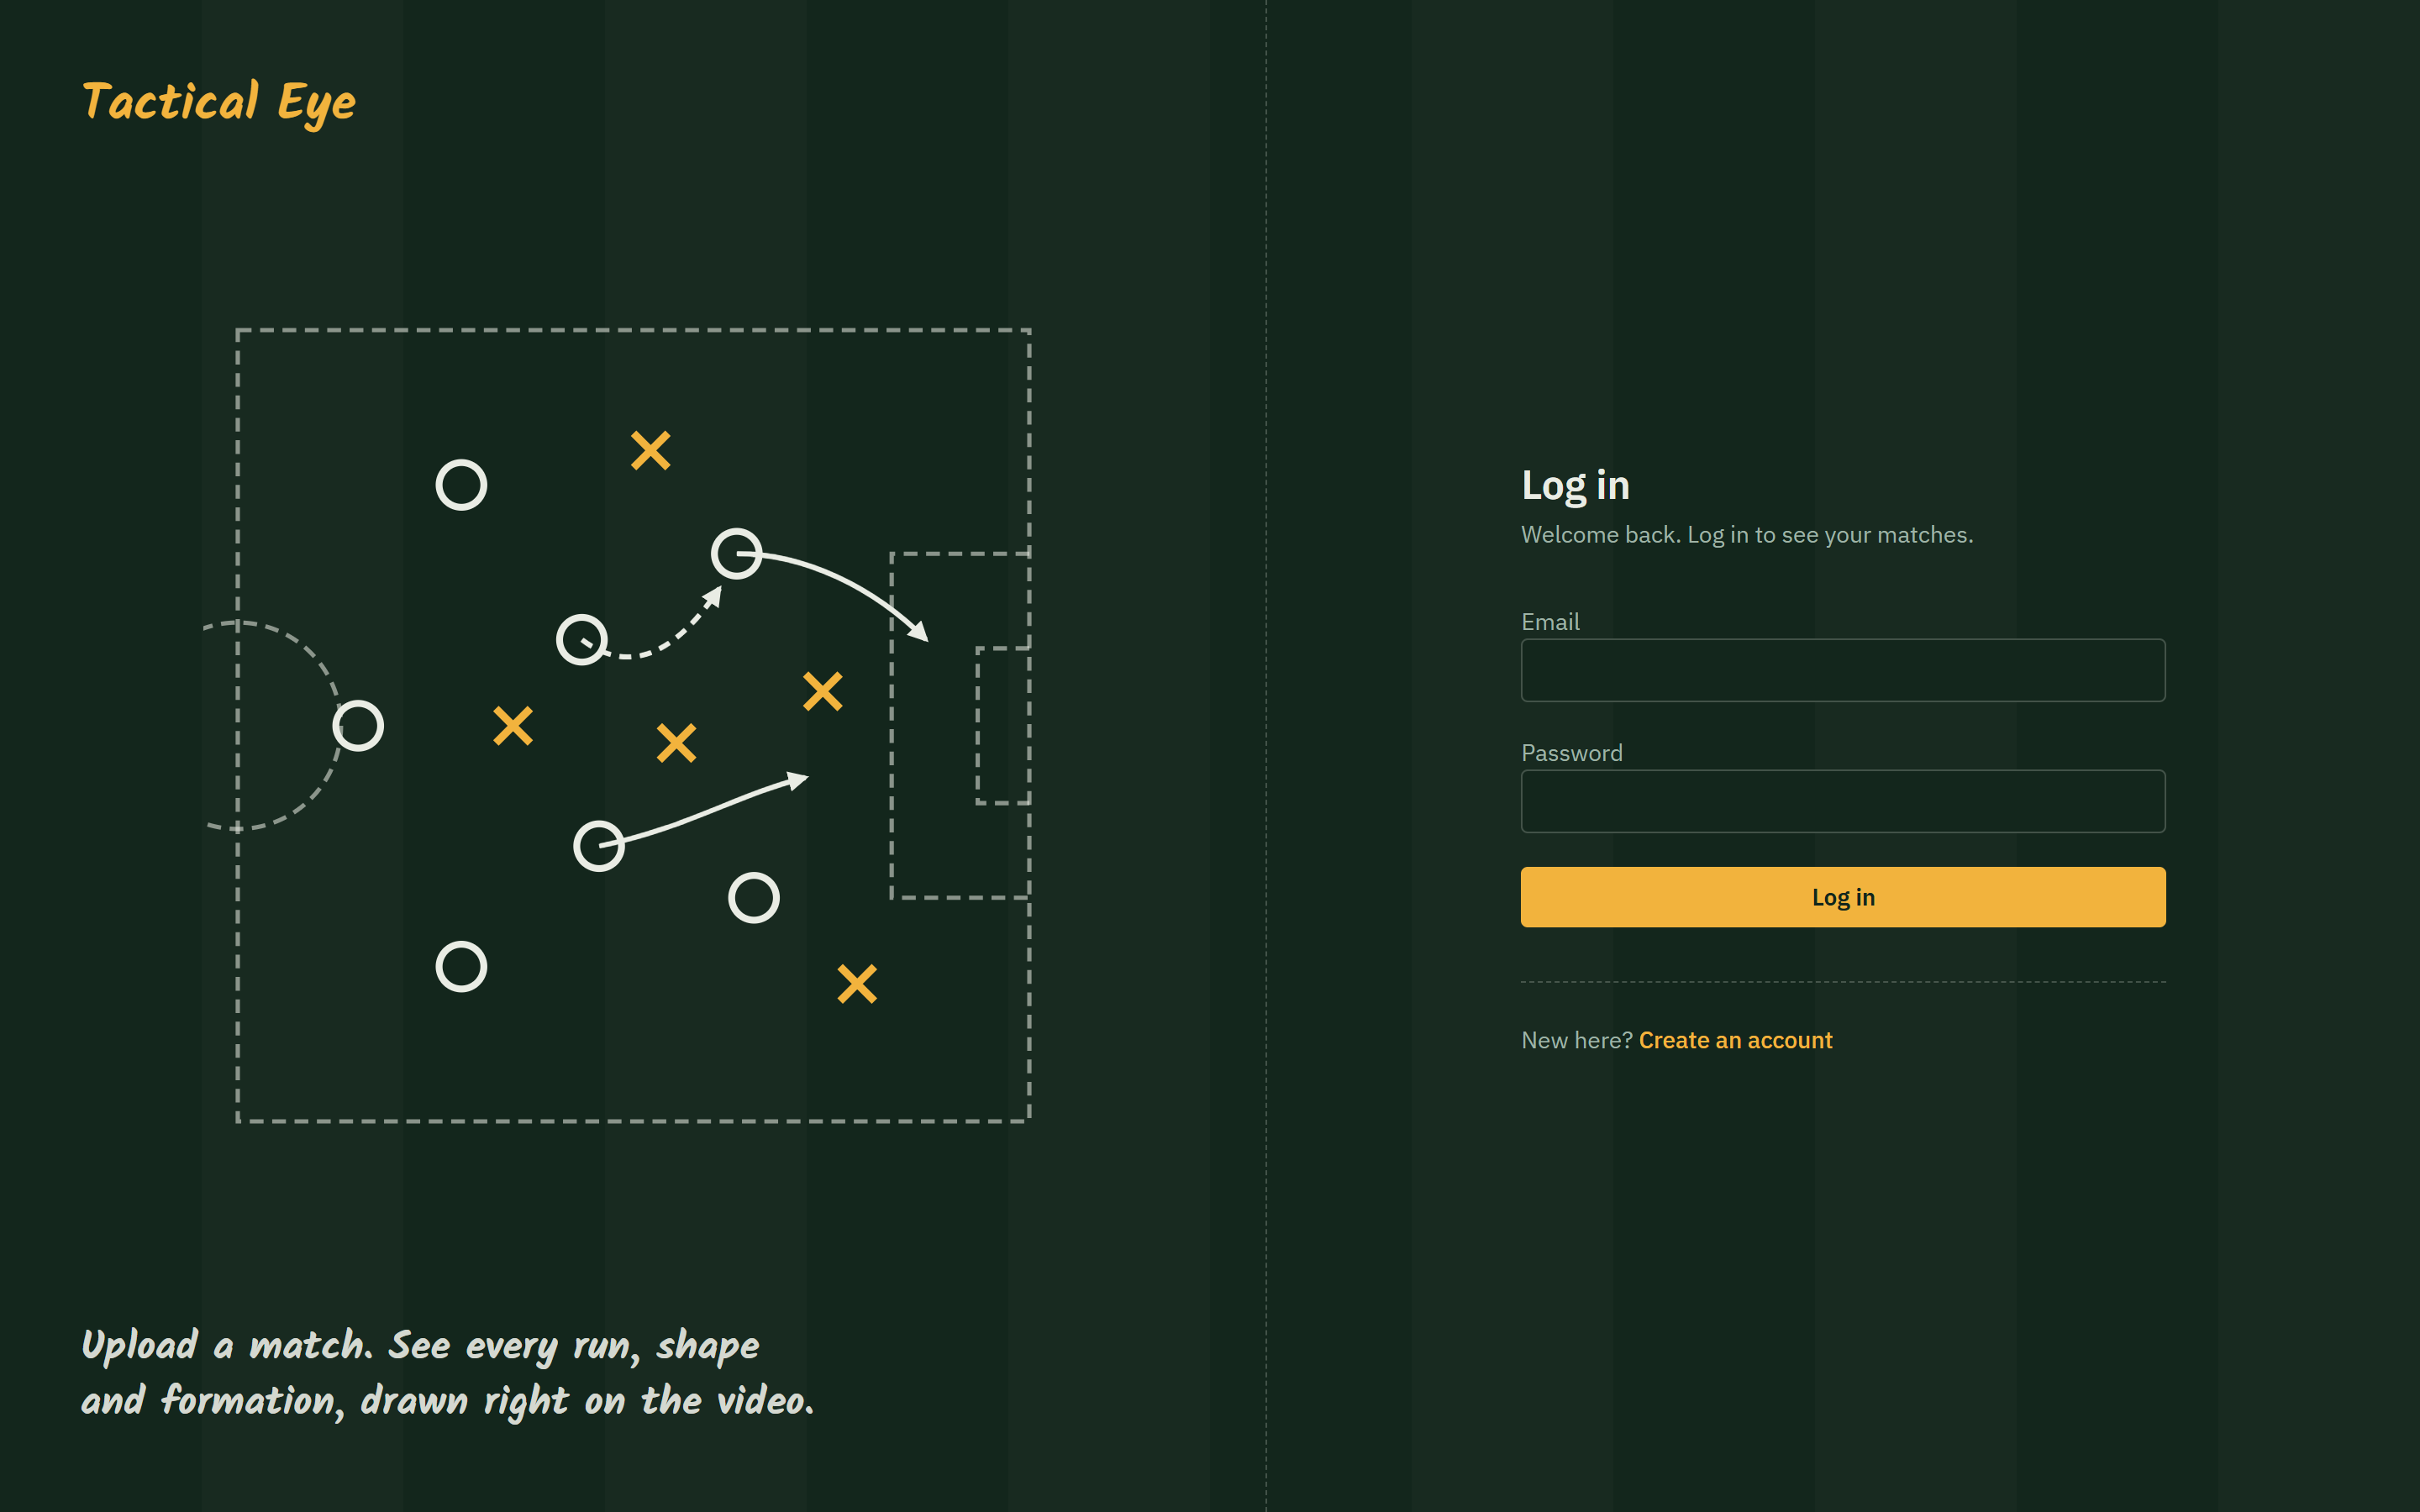
\includegraphics[width=\textwidth]{01_login}
		\caption{Log in}
		\label{fig:login}
	\end{subfigure}
	\hfill
	\begin{subfigure}{0.49\textwidth}
		\centering
		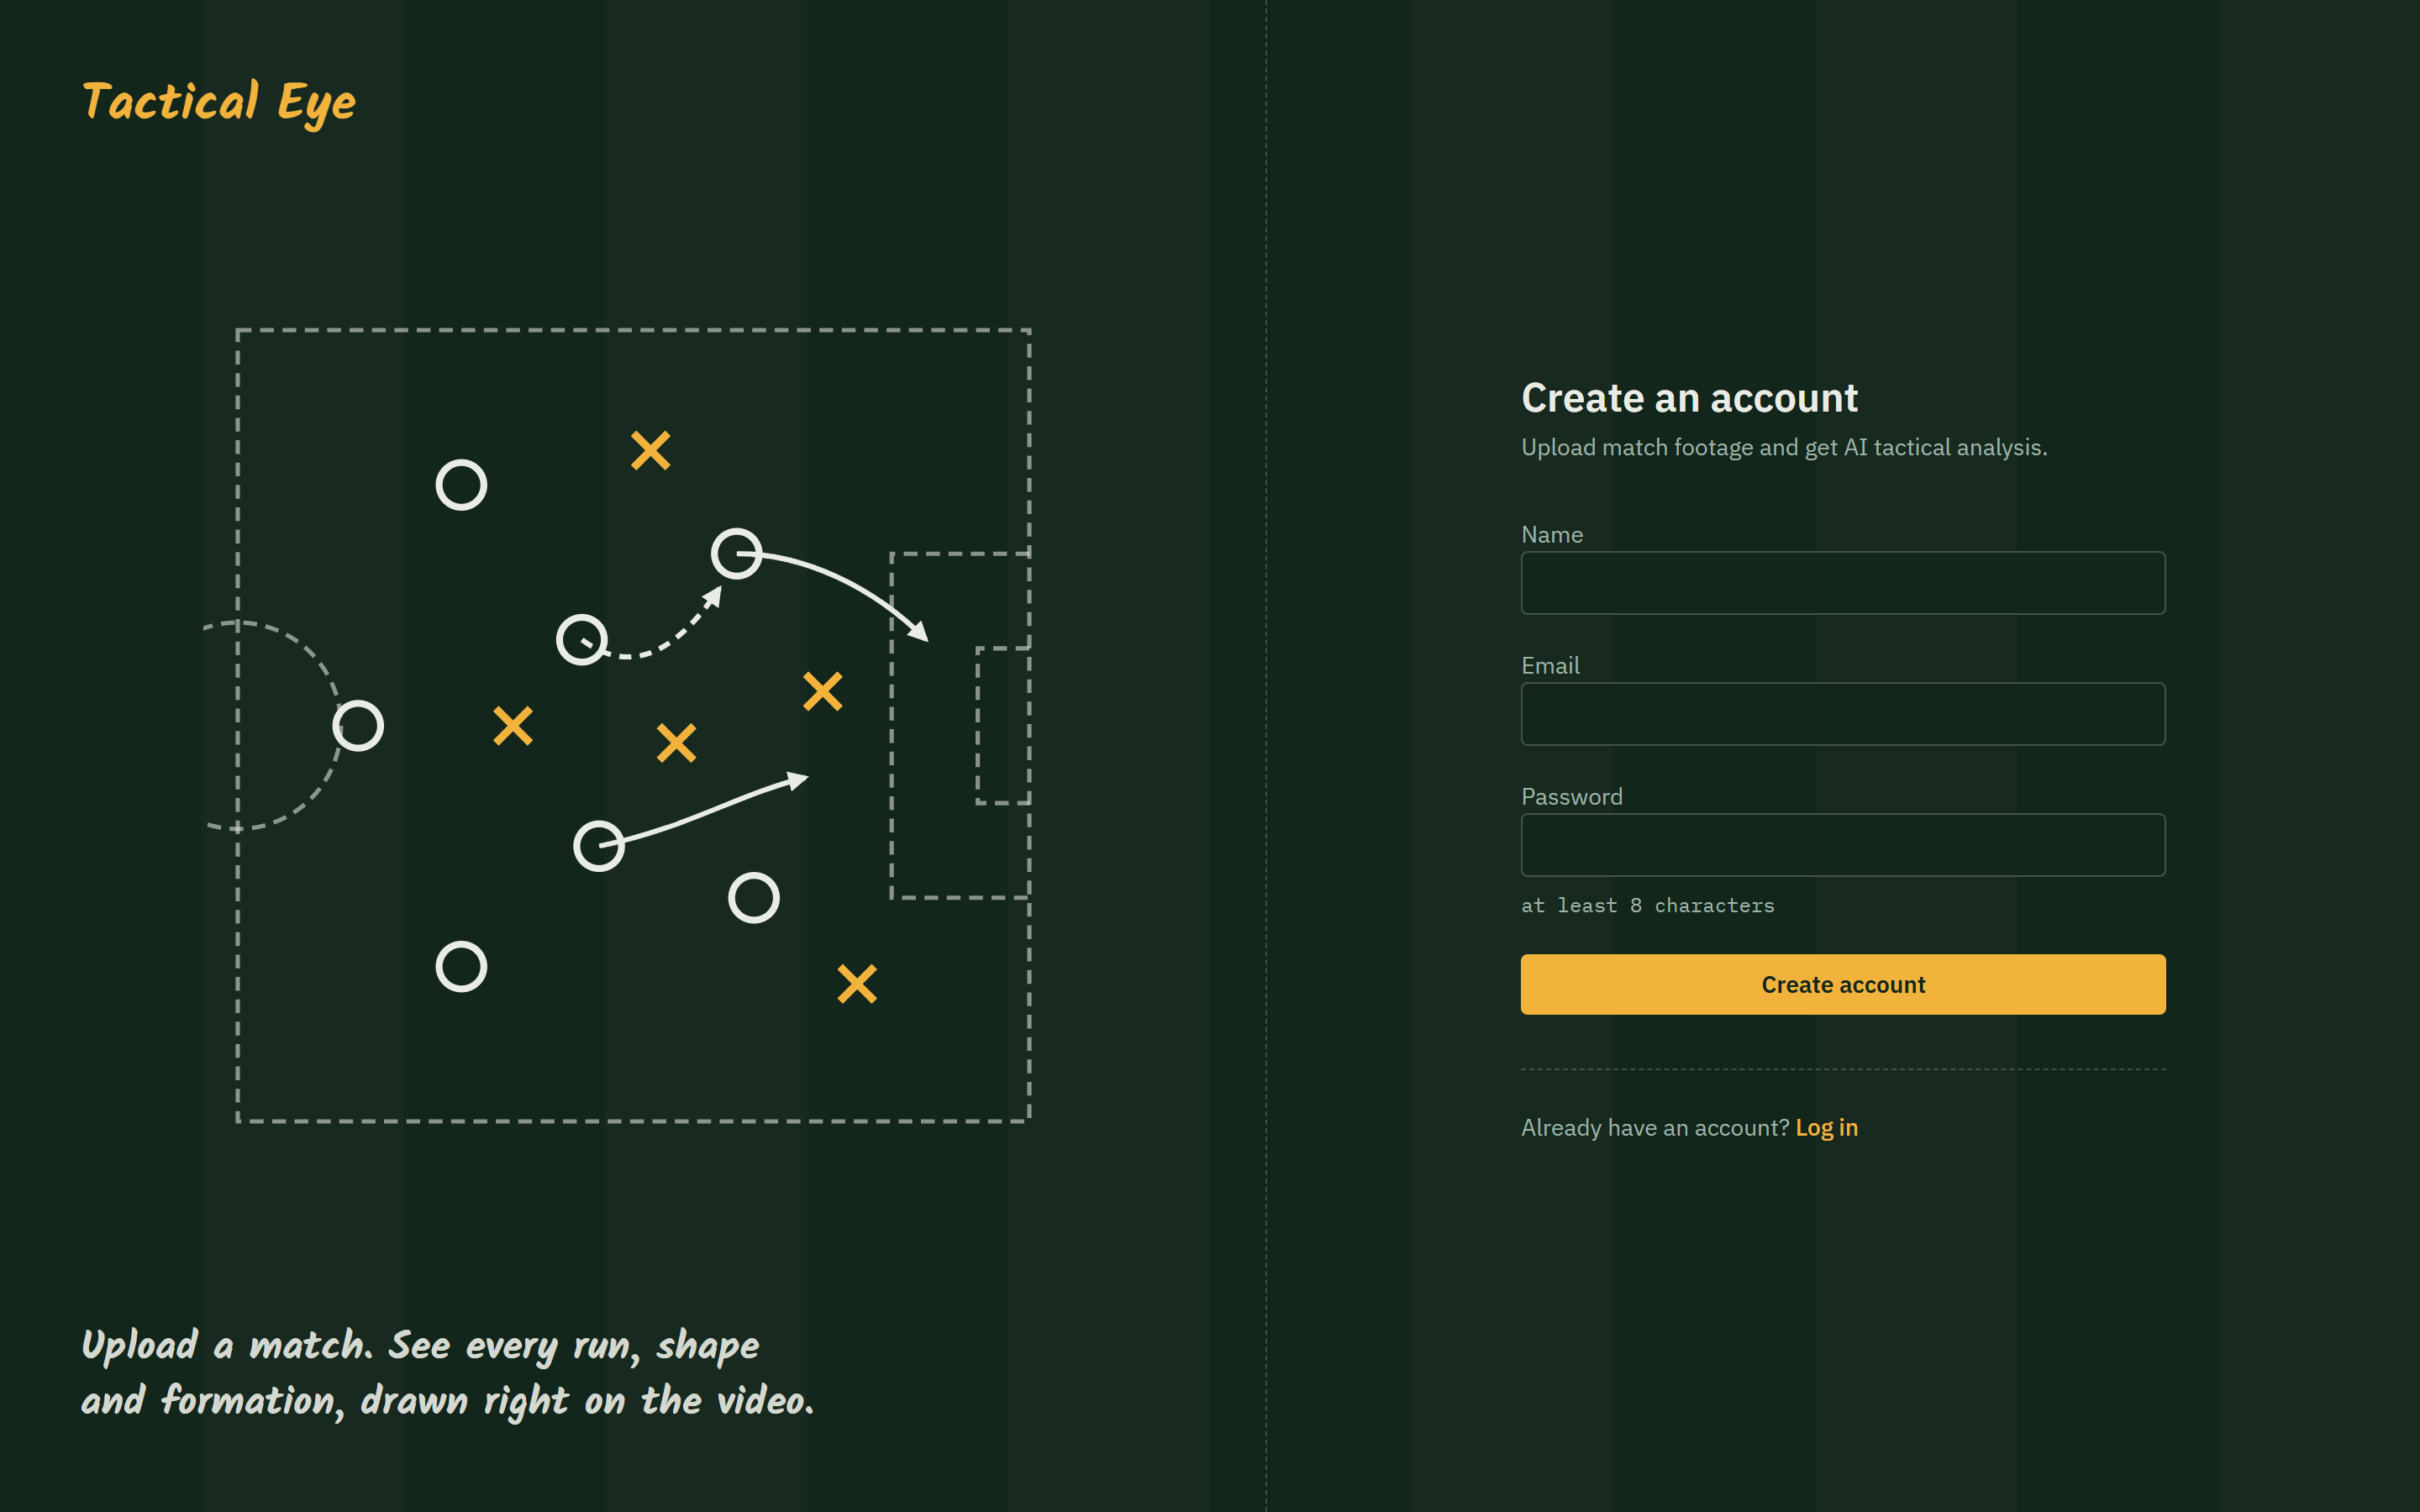
\includegraphics[width=\textwidth]{03_register}
		\caption{Create an account}
		\label{fig:register}
	\end{subfigure}
	\caption{The log-in and registration pages}
	\label{fig:auth-pages}
\end{figure}

A wrong e-mail address or password shows \emph{Invalid email or password} (\autoref{fig:login-error}). The message deliberately does not reveal whether the e-mail address is registered. A session lasts seven days; after that, or after \emph{Log out}, the user logs in again.

\begin{figure}[H]
	\centering
	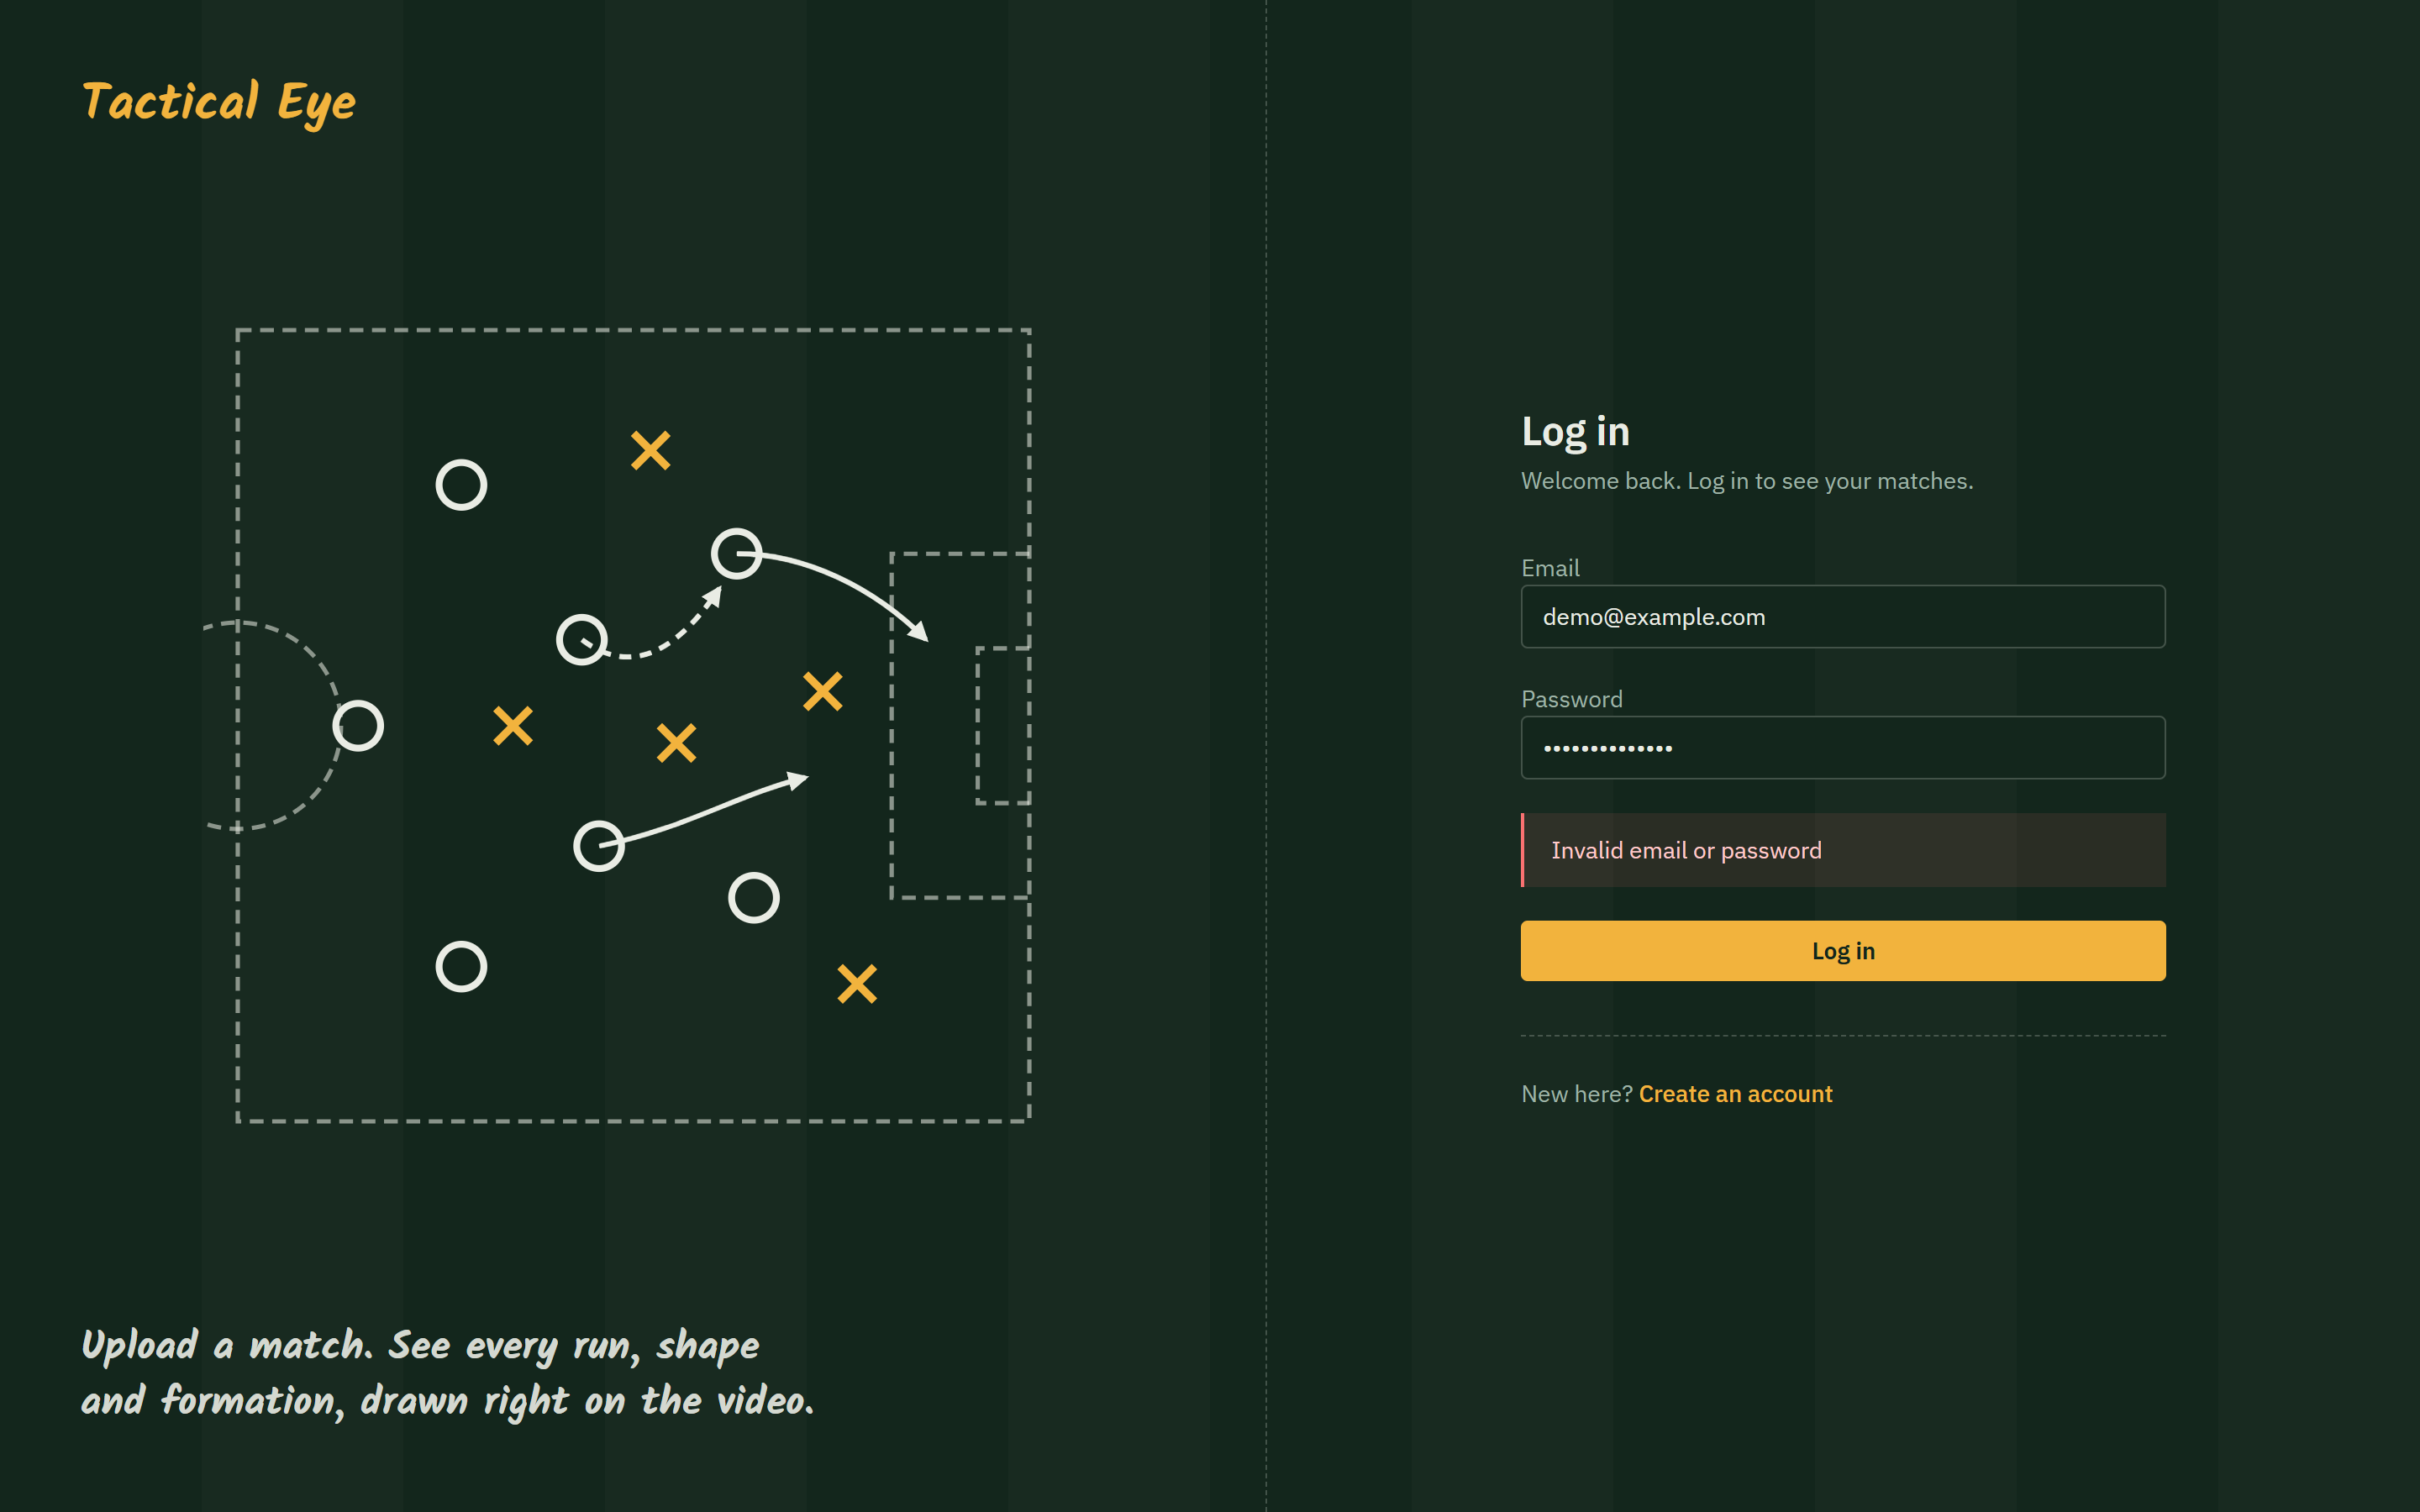
\includegraphics[width=0.75\textwidth]{02_login_error}
	\caption{A failed log-in attempt}
	\label{fig:login-error}
\end{figure}

\subsection{Navigation}

After logging in, every page has the same slim header: the \emph{Tactical Eye} logo, which leads to the match list, the \emph{Matches} and \emph{Upload} links, the user's name and \emph{Log out}. The dashboard is a single-page application, so moving between pages does not reload the browser window, and the browser's back and forward buttons work as usual.

\section{The match list}

The \emph{Matches} page (\autoref{fig:matches}) lists the user's uploads as rows, newest first. Each row shows the title, the upload date, the file size and the analysis mode, a handwritten status note (\autoref{tab:status}), and for finished matches each team's kit colour and its most frequent formation. \emph{+ Upload a match} opens the upload page; clicking a row opens the match.

\begin{figure}[H]
	\centering
	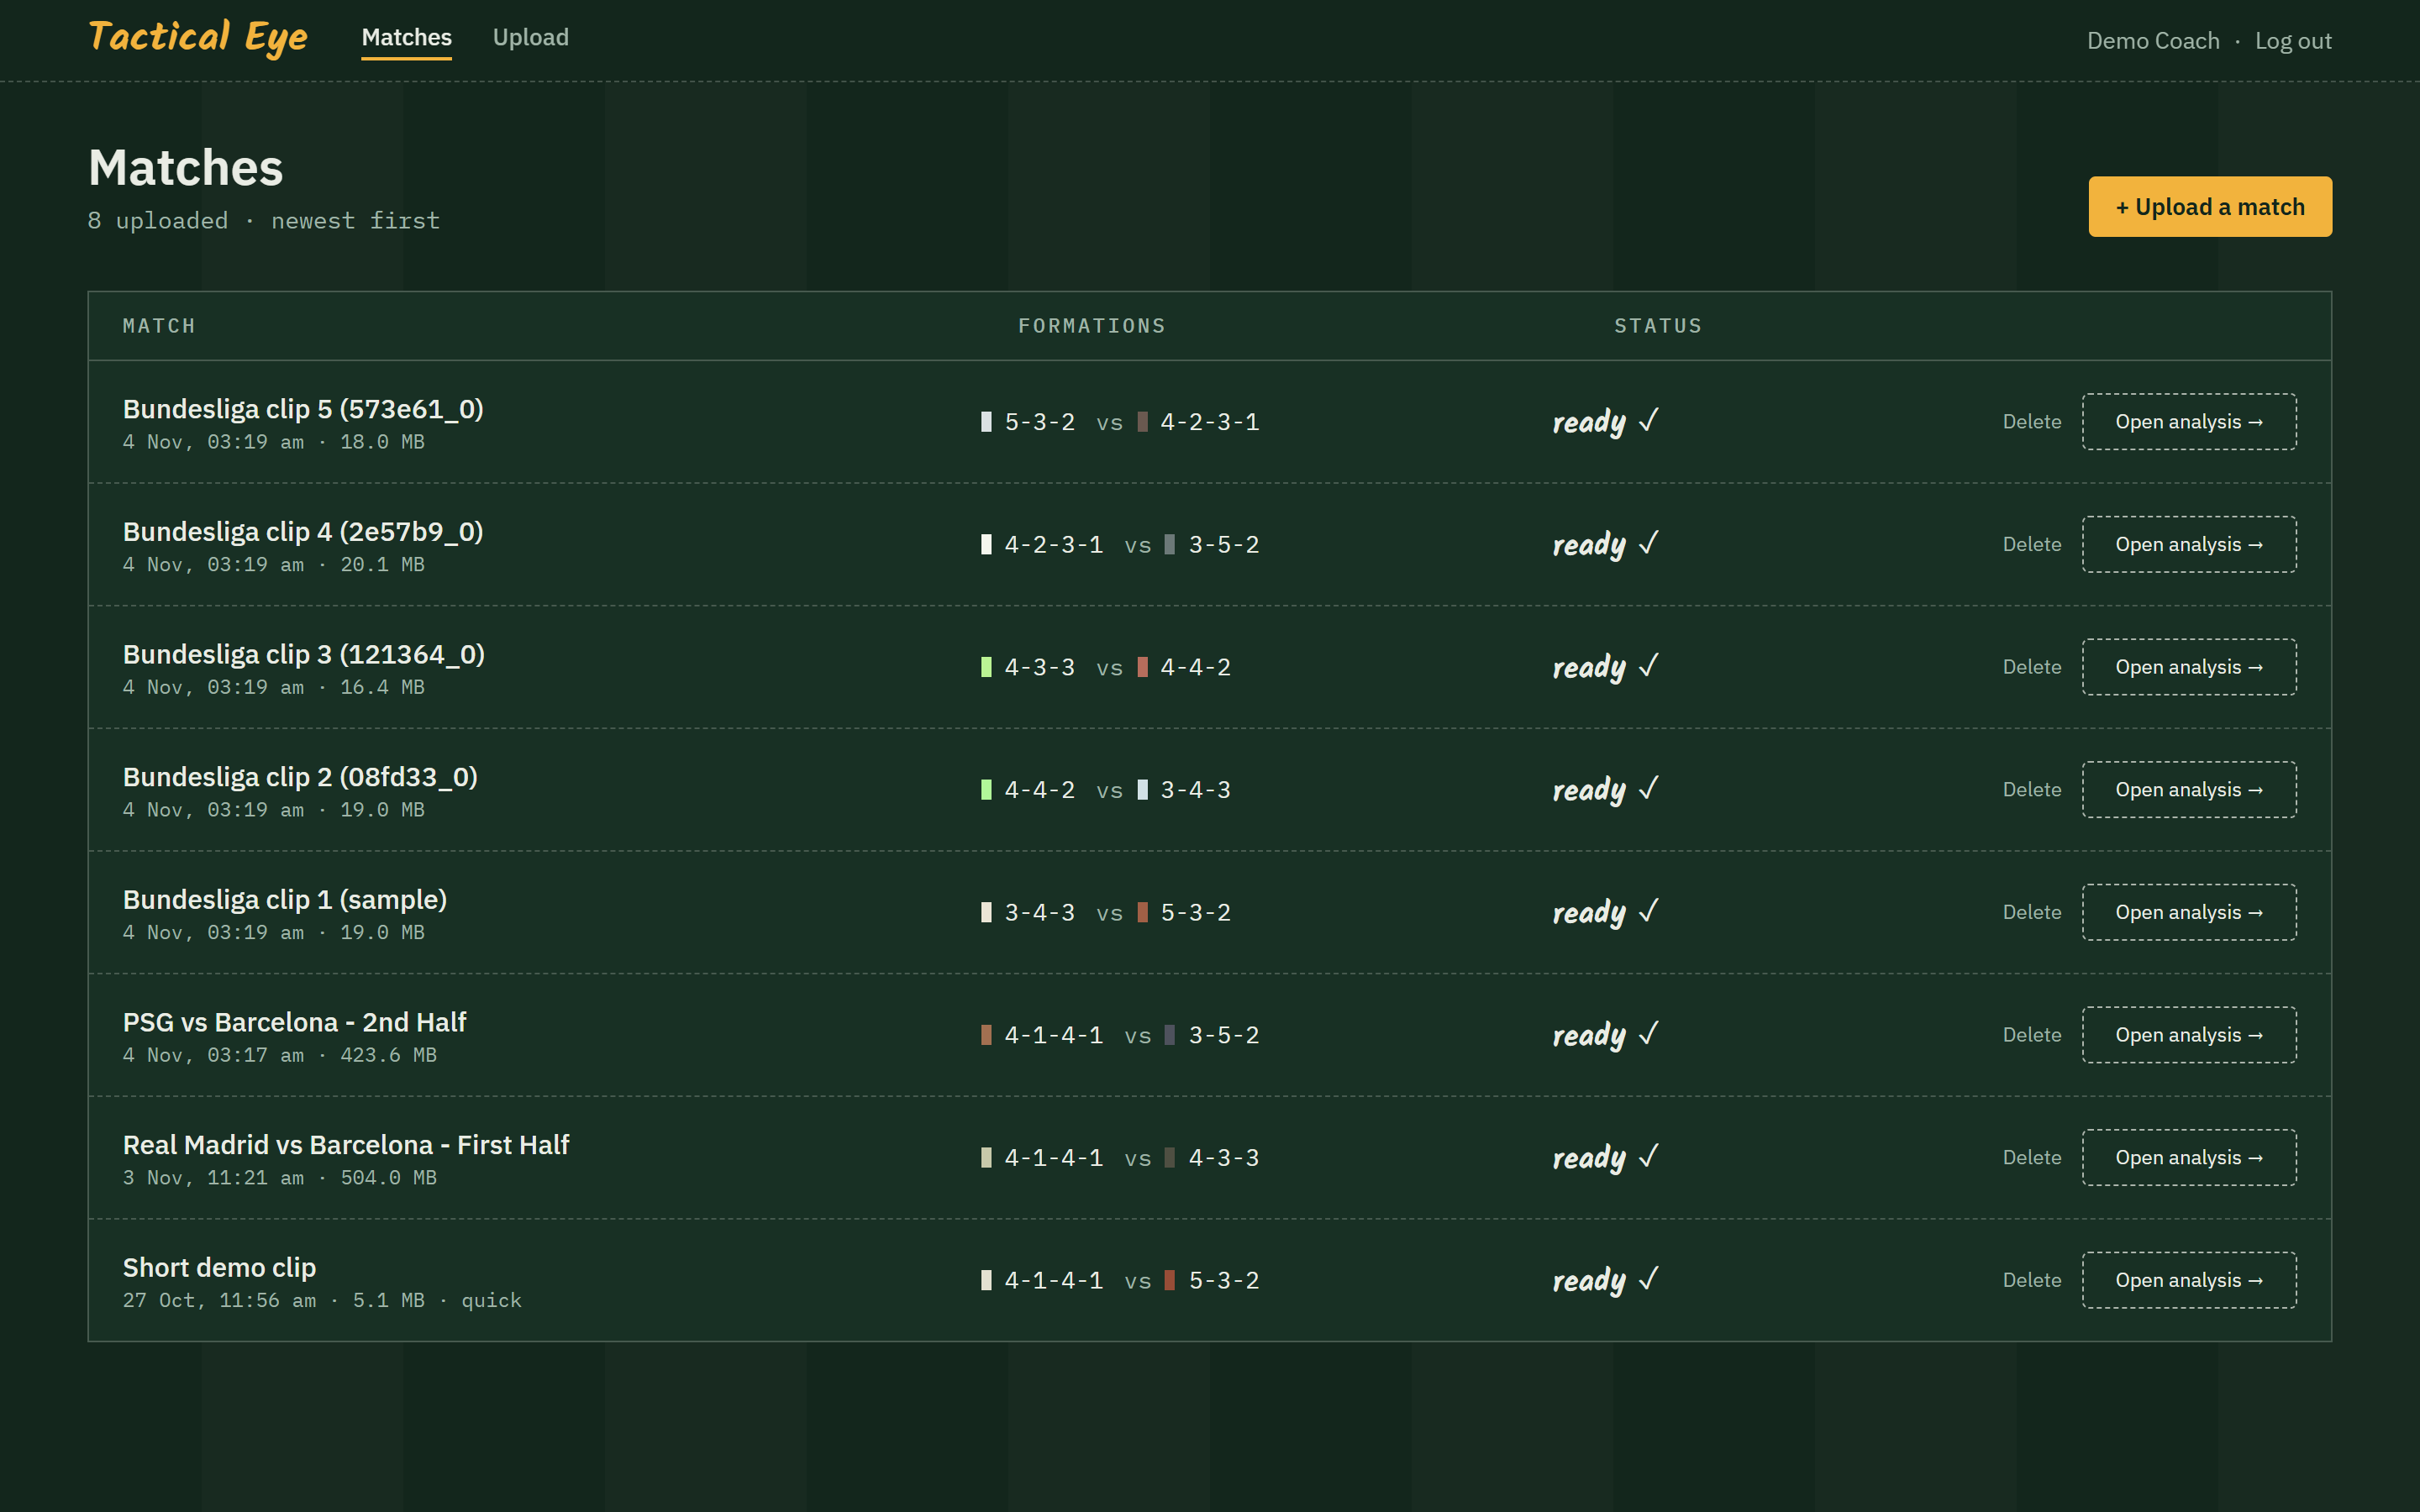
\includegraphics[width=\textwidth]{04_matches}
	\caption{The match list with two analysed halves and the five demo clips}
	\label{fig:matches}
\end{figure}

\begin{table}[H]
	\centering
	\begin{tabular}{|p{0.18\textwidth}|p{0.74\textwidth}|}
		\hline
		\textbf{Status} & \textbf{Meaning} \\
		\hline
		queued\dots & The video is stored and waits for a free worker. Videos are analysed one at a time, in upload order. \\
		\hline
		analysing\dots & A worker is processing the video; the row shows a progress bar and the current step. \\
		\hline
		ready \checkmark & The analysis is finished and can be opened. \\
		\hline
		failed $\times$ & The analysis could not be completed; the row shows the reason (\autoref{sec:messages}). \\
		\hline
		cancelled -- & The user stopped the analysis; it can be started again with \emph{Re-analyse}. \\
		\hline
	\end{tabular}
	\caption{Status notes}
	\label{tab:status}
\end{table}

The list updates itself: progress bars move, statuses change and new matches appear without reloading the page, because the server pushes every change to the browser.

\section{Uploading a match}

The upload page (\autoref{fig:upload-empty}) leads through three numbered steps, with tips for good results on the right.

\begin{enumerate}
	\item \emph{Choose the video}: drag a file onto the dashed area or click it to pick one. MP4, MOV, M4V, MKV, WebM and AVI files are accepted, up to 1\,GB, which is enough for a full half (\autoref{fig:upload-ready}). Any codec and frame rate works; the server converts the video for the browser.
	\item \emph{Give it a name}: the title is filled in from the file name and can be up to 120 characters long.
	\item \emph{Pick the analysis mode} (\autoref{tab:modes}).
\end{enumerate}

Then \emph{Upload and analyse} sends the file with a progress bar. When the upload completes, the dashboard opens the new match's page.

\begin{figure}[H]
	\centering
	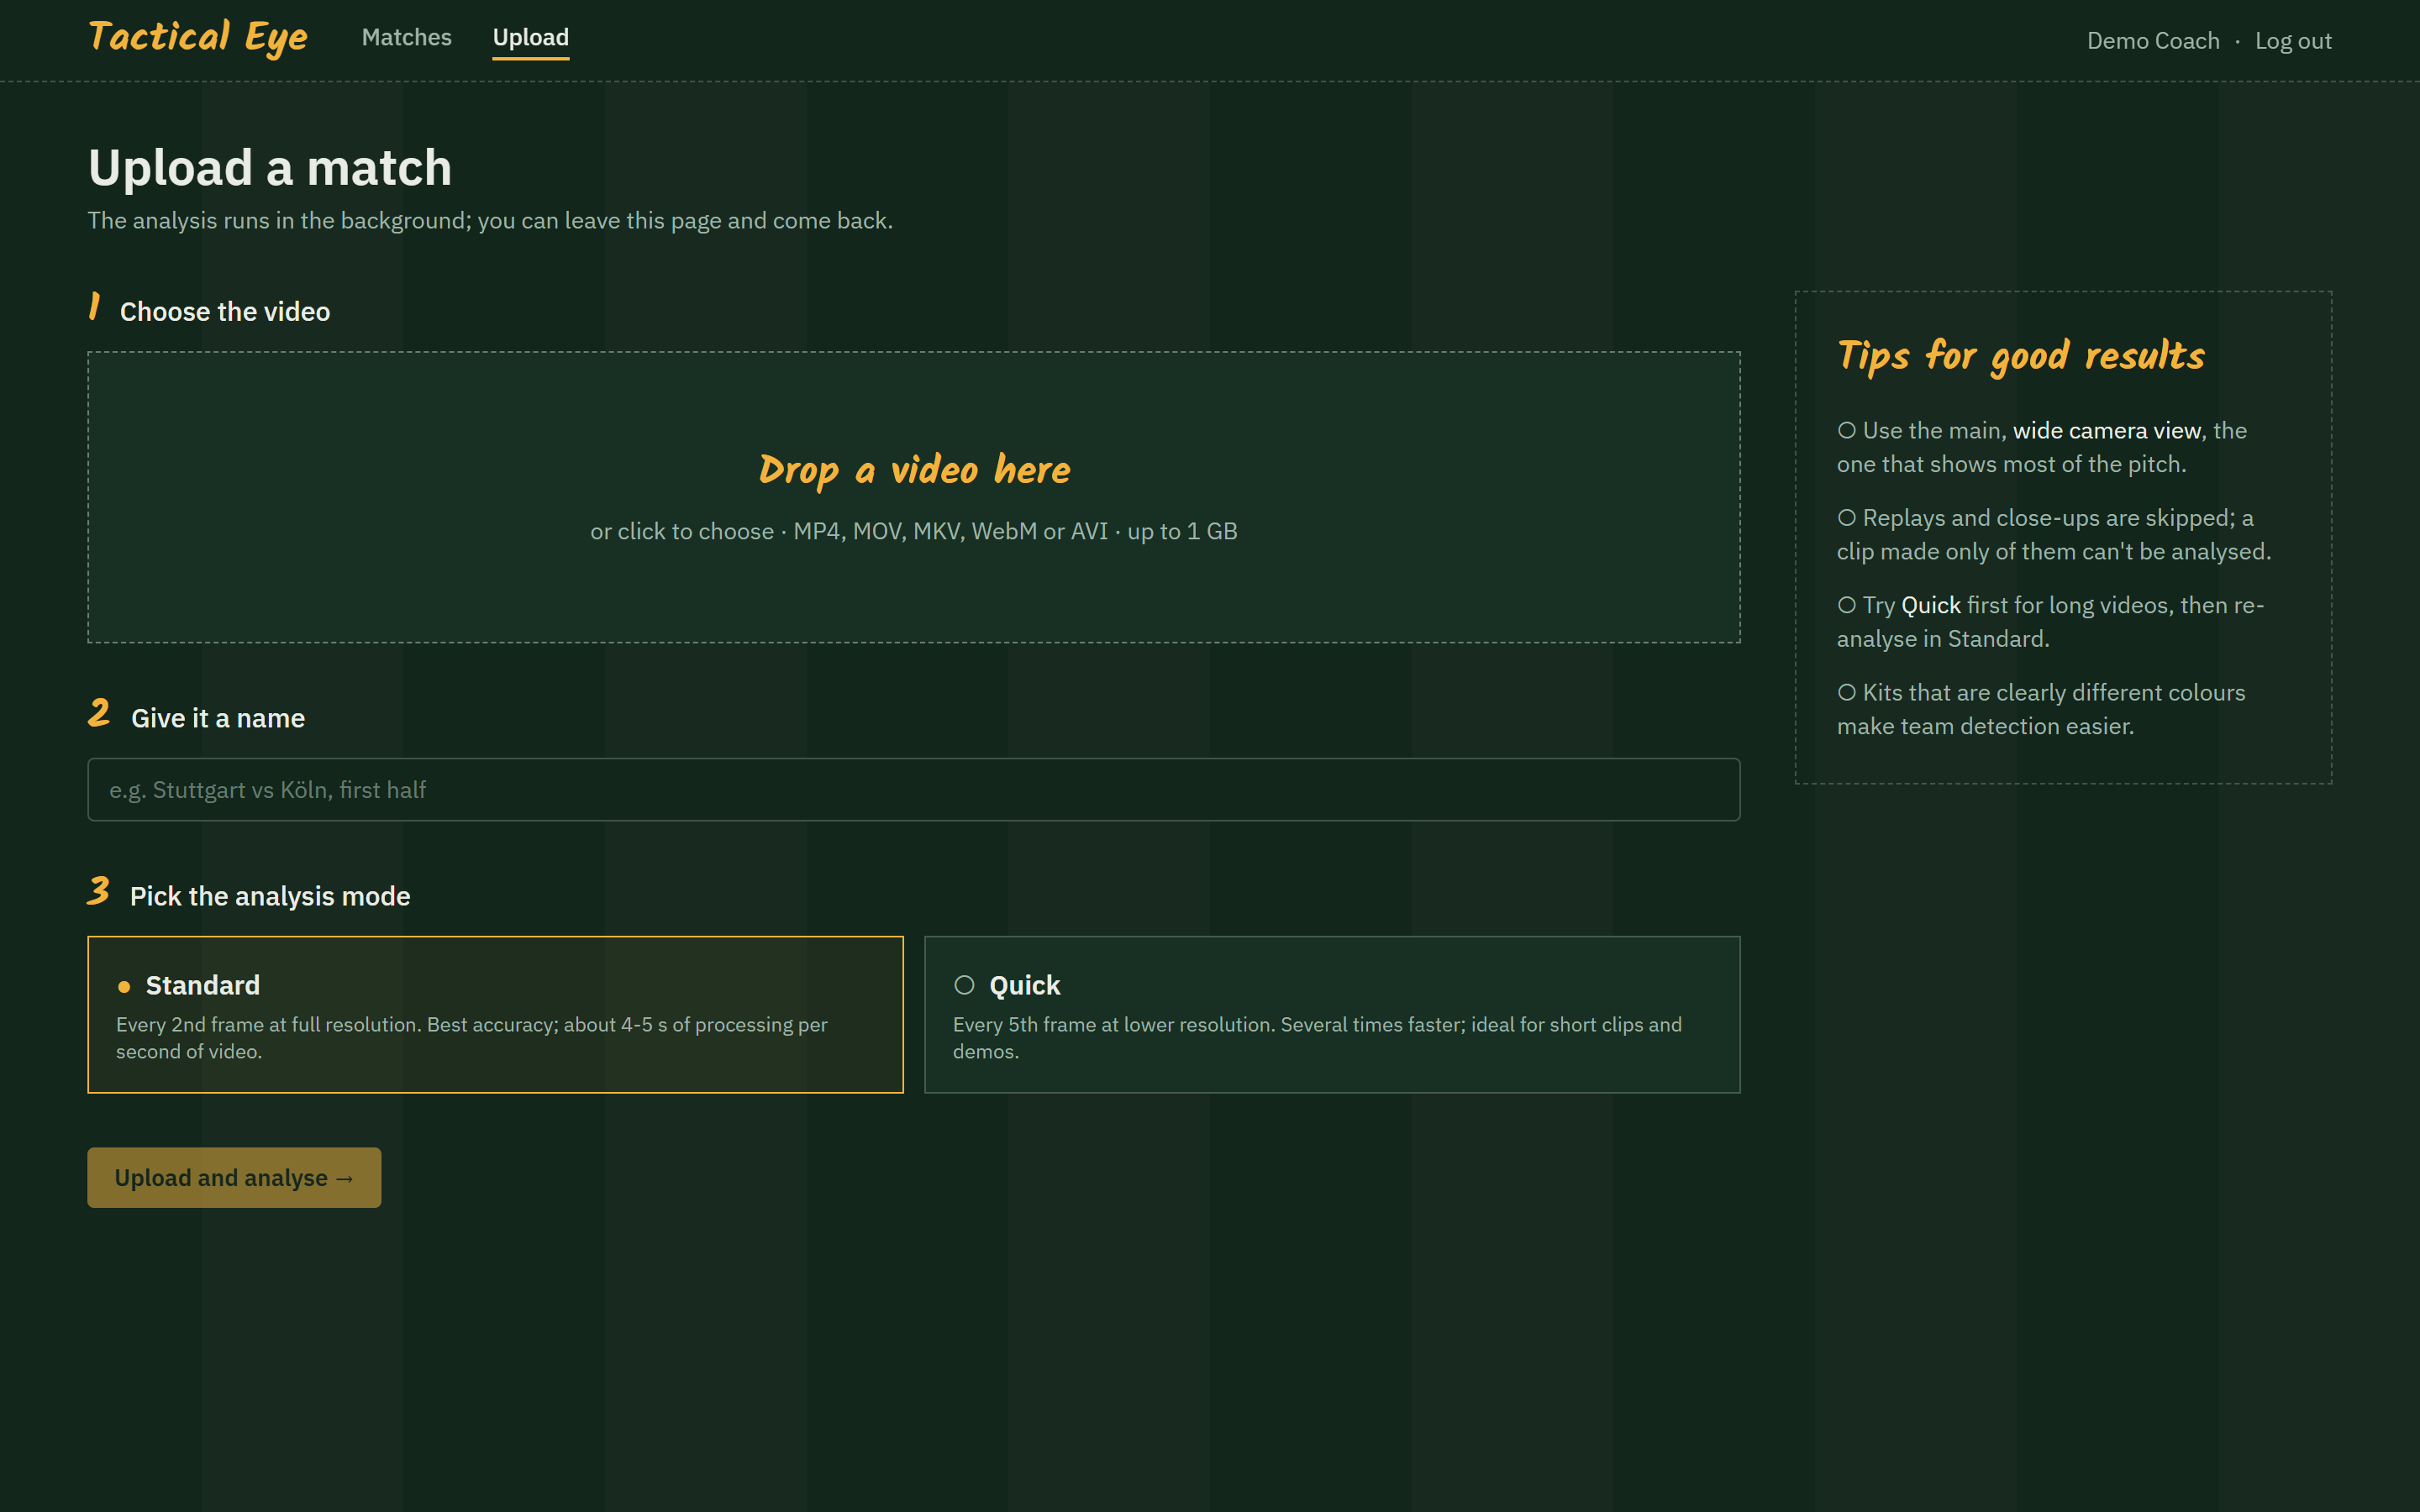
\includegraphics[width=\textwidth]{05_upload_empty}
	\caption{The upload page before a file is chosen}
	\label{fig:upload-empty}
\end{figure}

\begin{figure}[H]
	\centering
	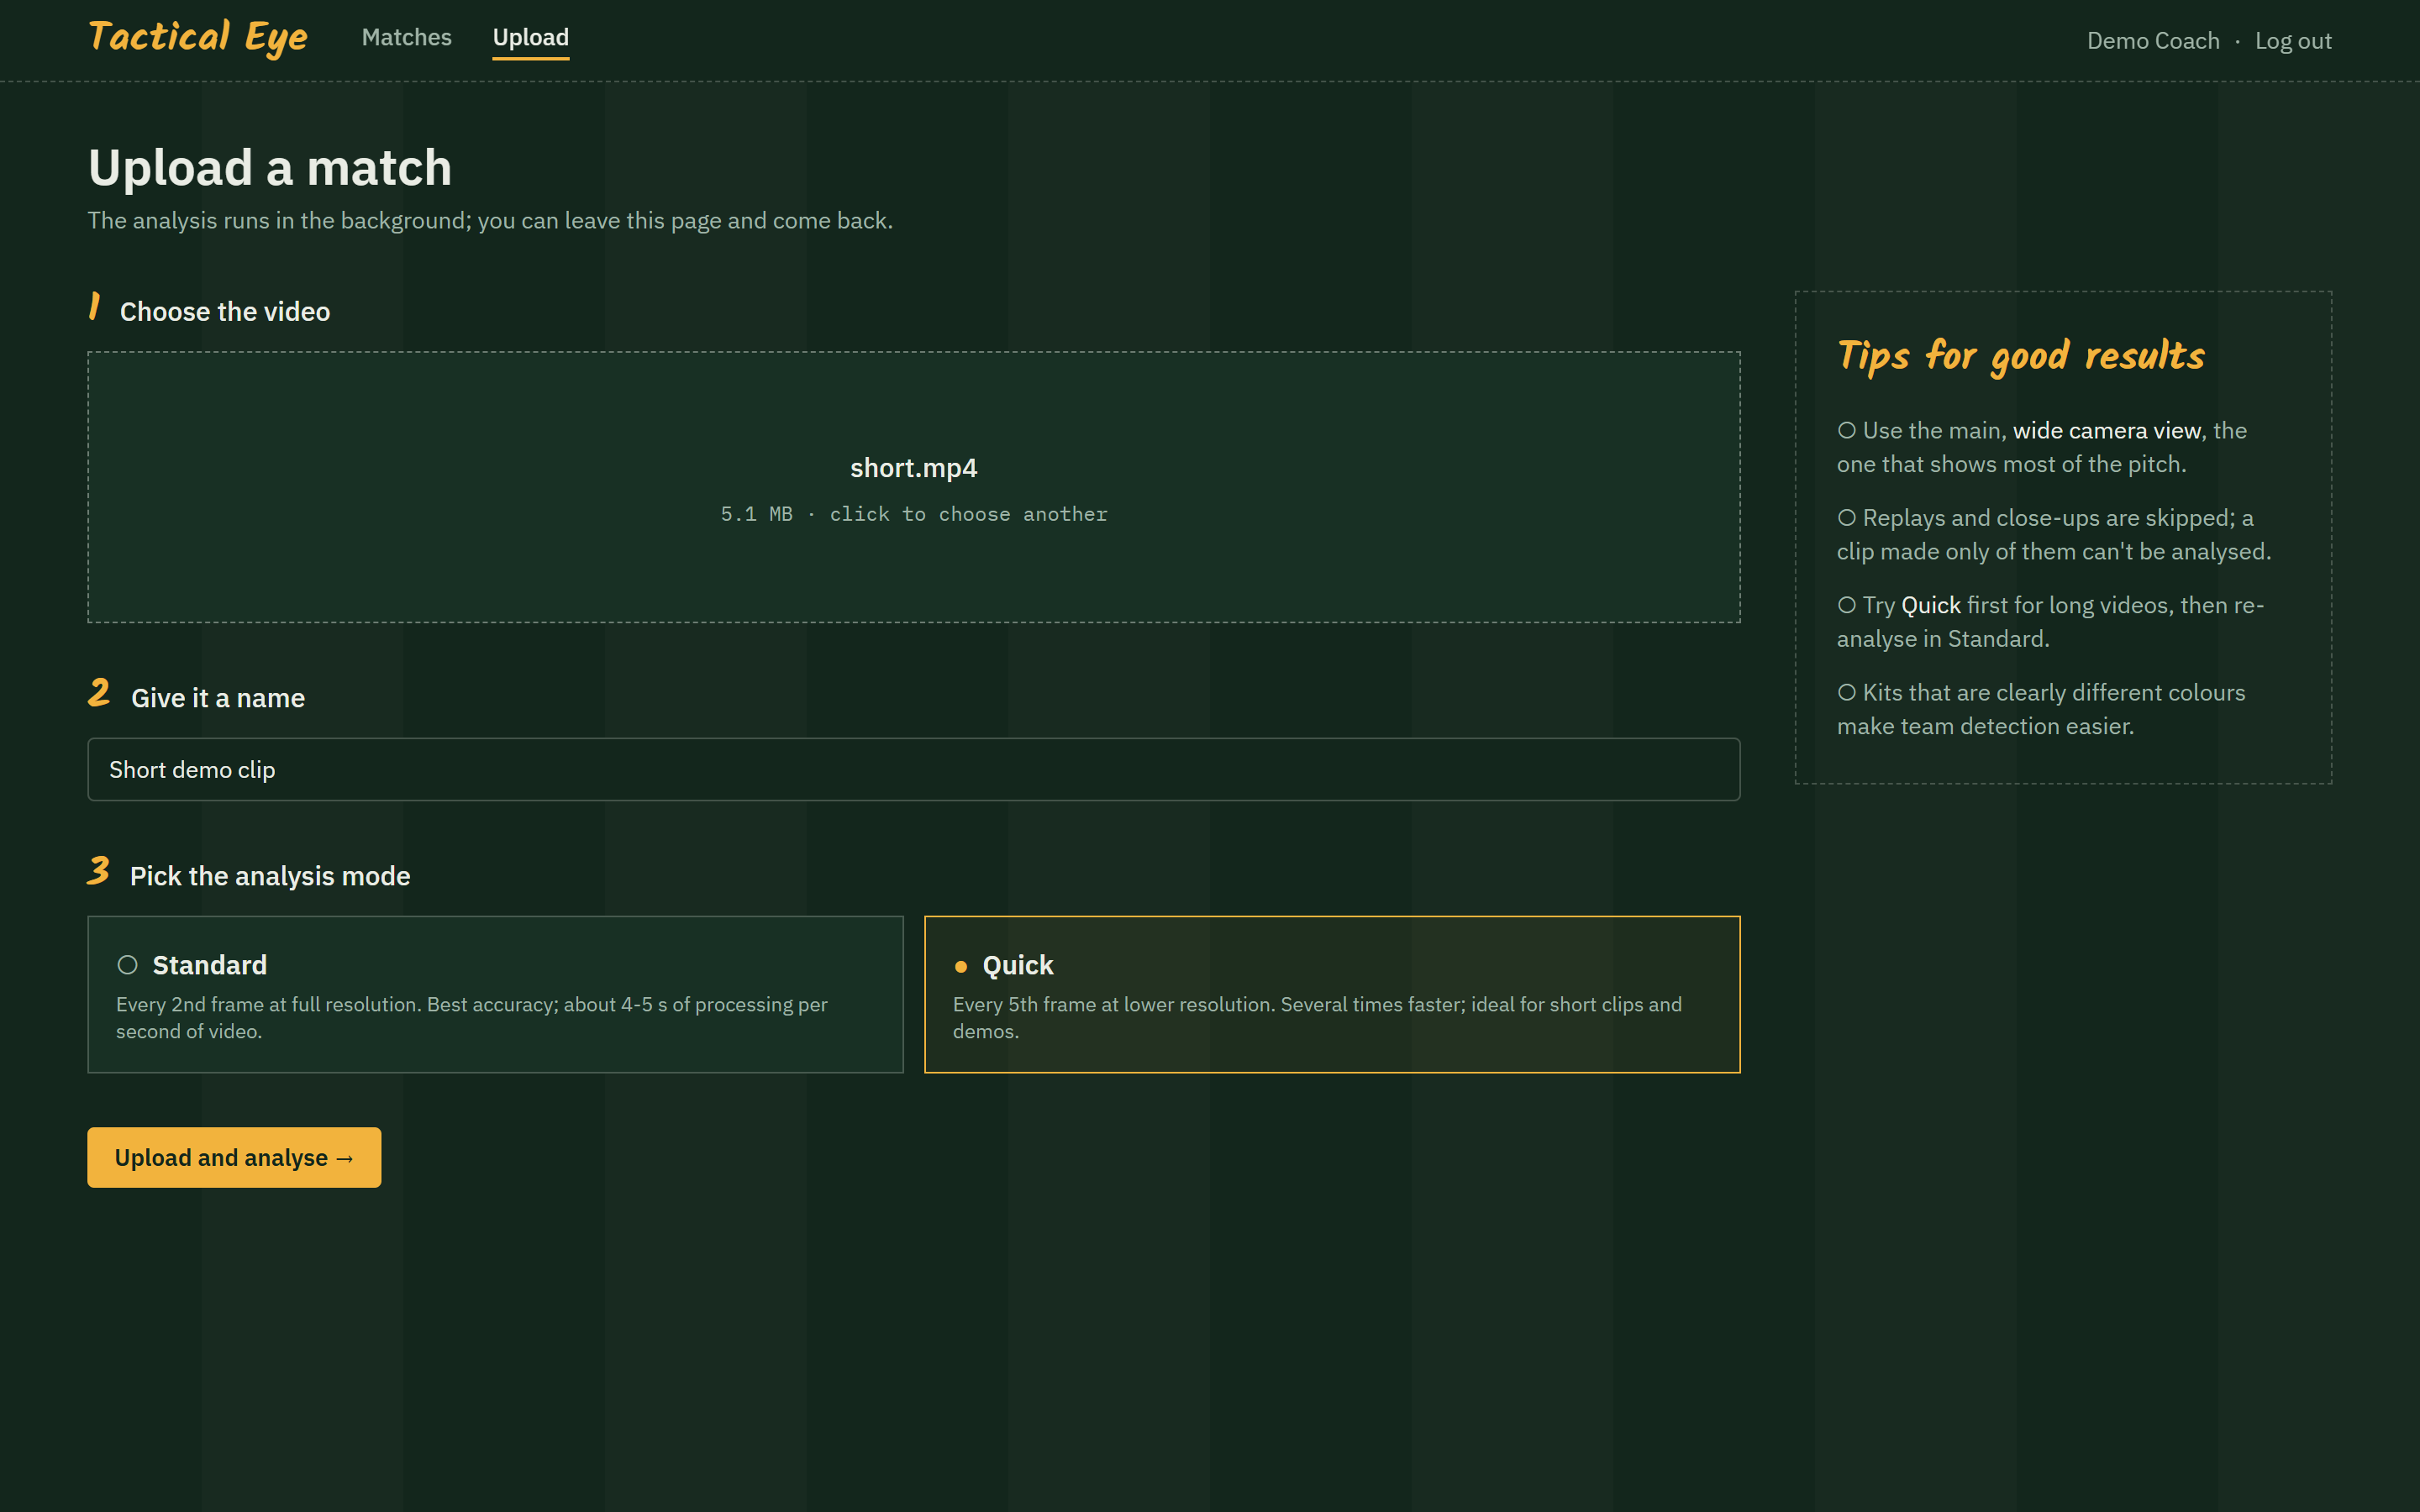
\includegraphics[width=\textwidth]{07_upload_ready}
	\caption{A file is chosen, the title is filled in and Quick mode is selected}
	\label{fig:upload-ready}
\end{figure}

\begin{table}[H]
	\centering
	\begin{tabular}{|p{0.13\textwidth}|p{0.38\textwidth}|p{0.40\textwidth}|}
		\hline
		\textbf{Mode} & \textbf{What it does} & \textbf{When to use it} \\
		\hline
		Standard & Analyses 12.5 frames per second of video (every 2nd frame at 25\,fps, every 4th at 50\,fps) at 1280-pixel detection resolution. & Best accuracy; the default, and the mode used for full halves on a GPU. \\
		\hline
		Quick & Analyses 5 frames per second at 960 pixels. & Several times faster, for short clips, previews and live demonstrations. The ball is found less often. \\
		\hline
	\end{tabular}
	\caption{Analysis modes}
	\label{tab:modes}
\end{table}

Footage from the main, wide camera gives the best results. Close-ups, replays and crowd shots contain no usable view of the pitch; the analysis skips them, but a video made mostly of them cannot be analysed (\autoref{sec:messages}).

Every upload is checked on the server. A file that is not really a video, for example a text file renamed to \texttt{.\allowbreak{}mp4}, is rejected with \emph{The file is not a valid video} and nothing is stored (\autoref{fig:upload-invalid}).

\begin{figure}[H]
	\centering
	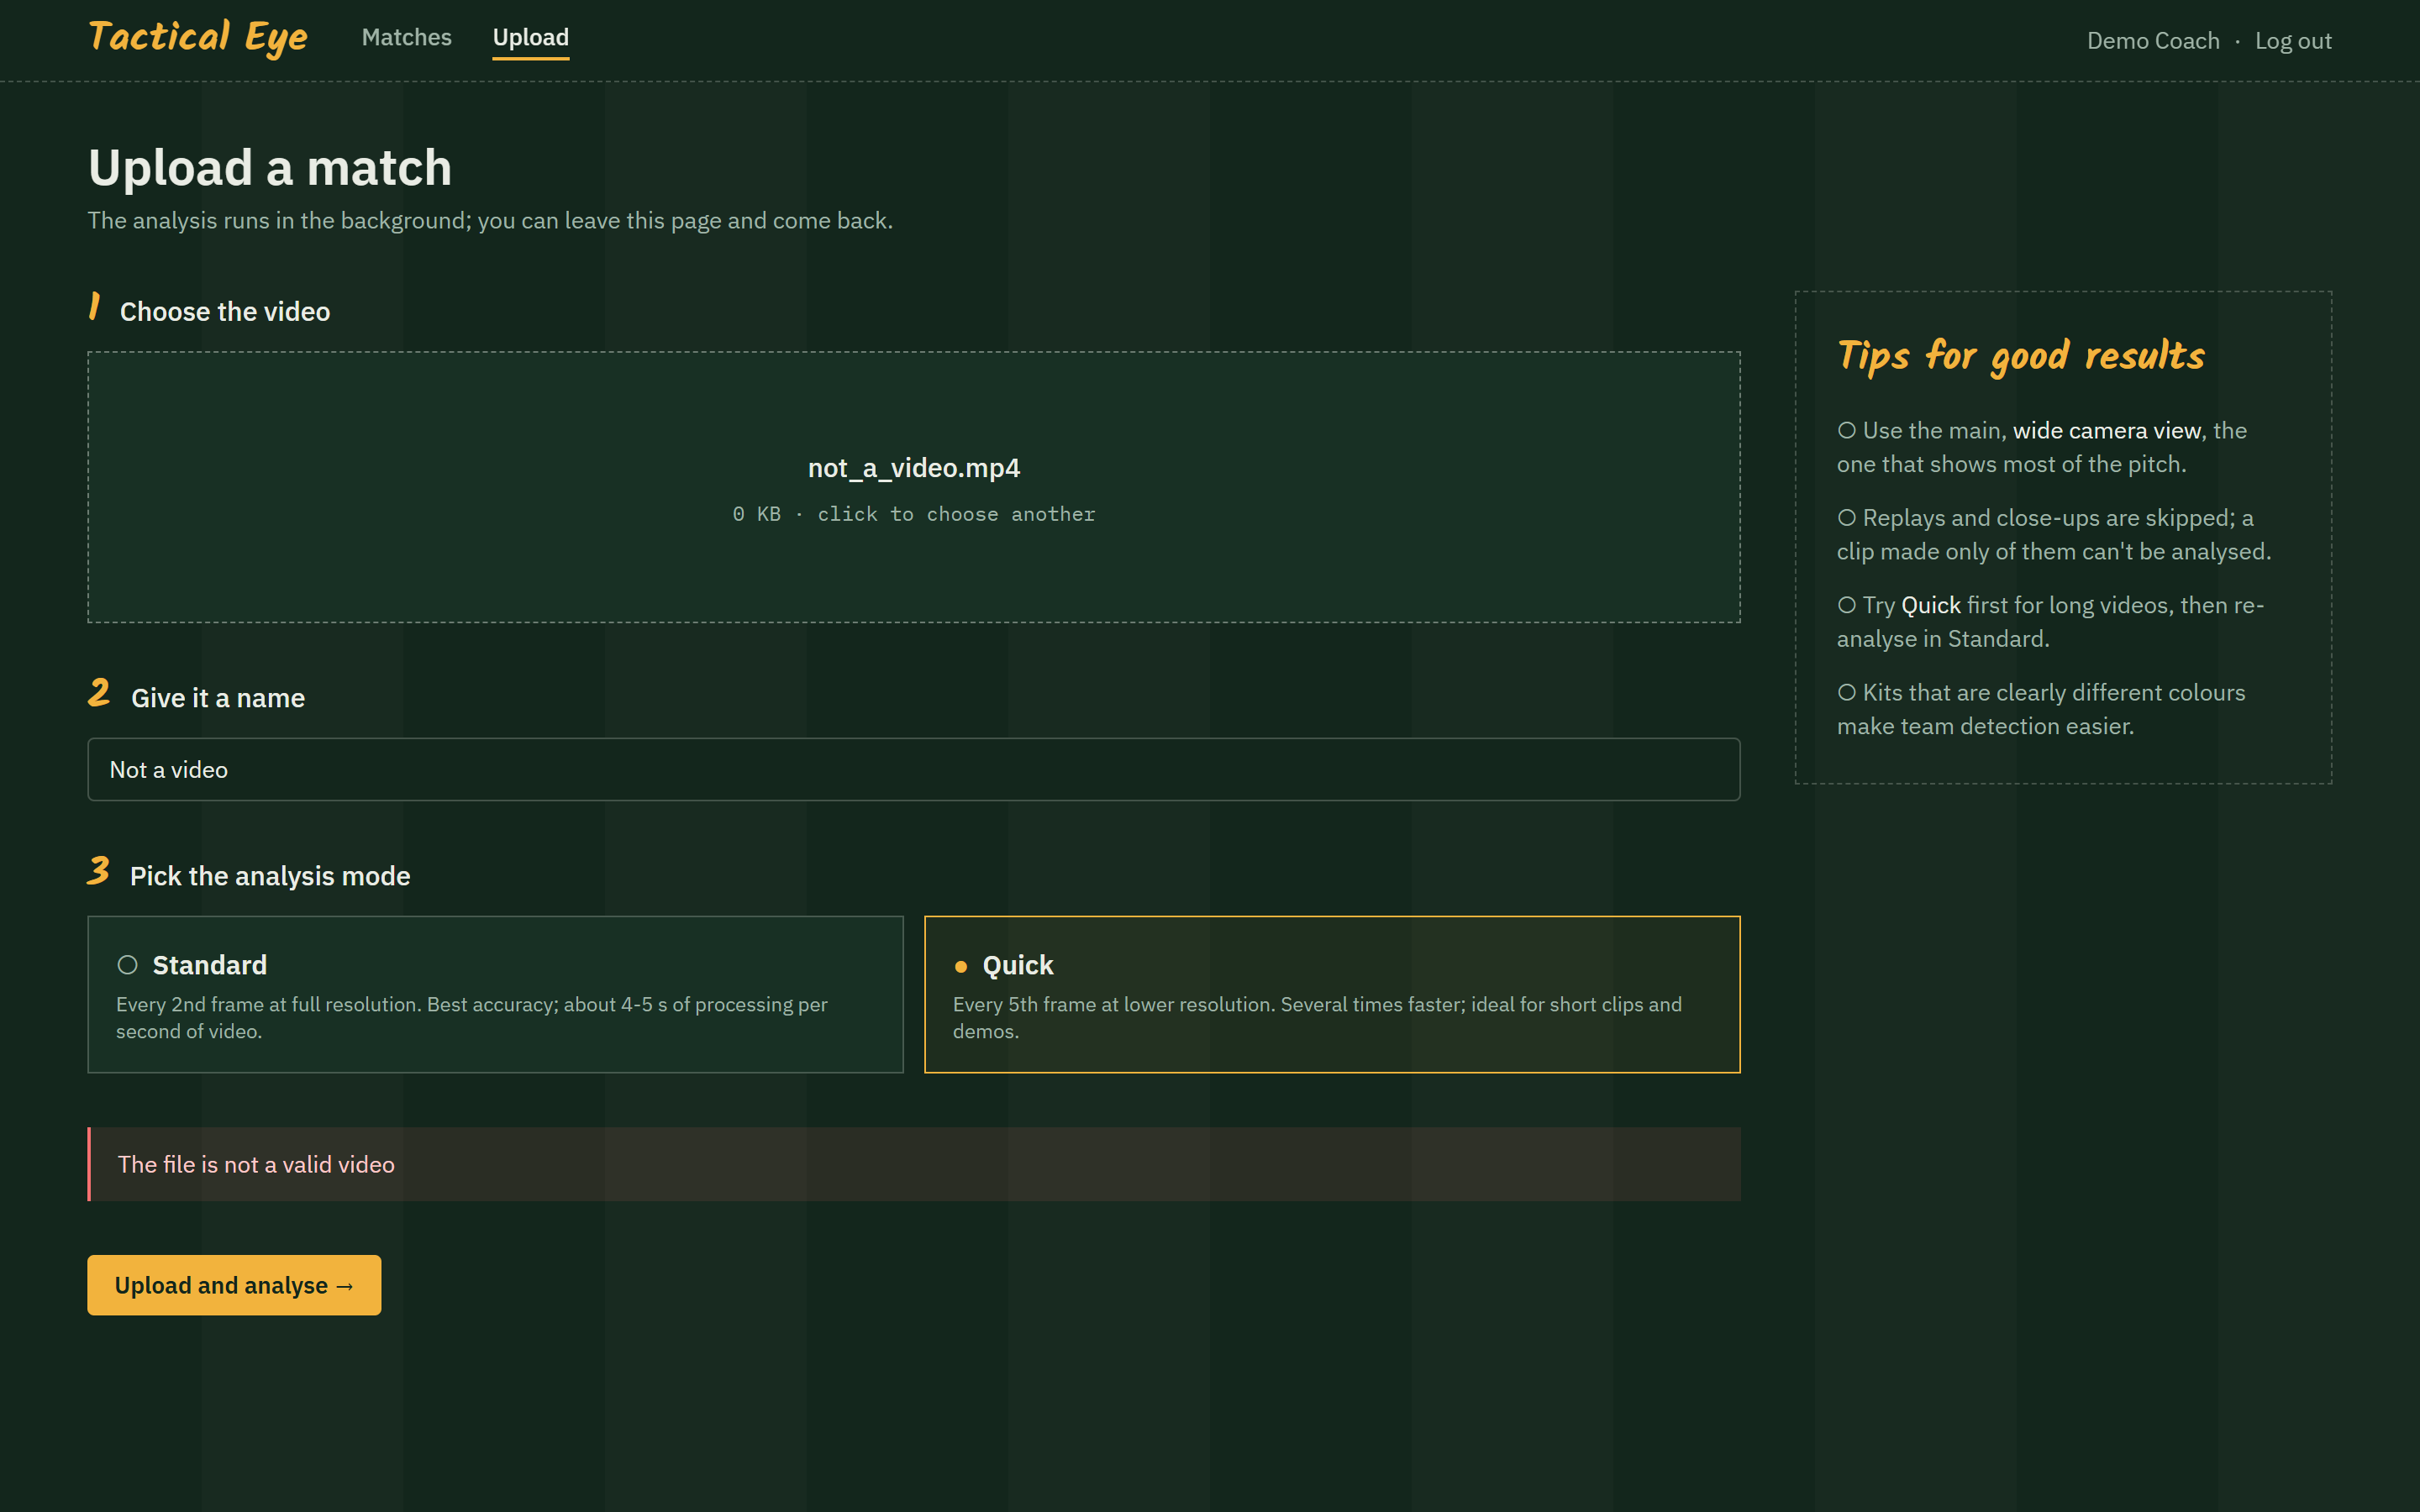
\includegraphics[width=\textwidth]{06_upload_invalid_file}
	\caption{A file that is not a video is rejected}
	\label{fig:upload-invalid}
\end{figure}

\section{Following and cancelling the analysis}

While a video is being analysed, its page shows a progress bar with the current step (\autoref{fig:in-progress}). The page updates live; the user can leave it, close the browser or upload more matches, and the analysis continues on the server. The match list shows the same progress in the match's row (\autoref{fig:list-progress}). \autoref{tab:steps} lists the steps.

\begin{figure}[H]
	\centering
	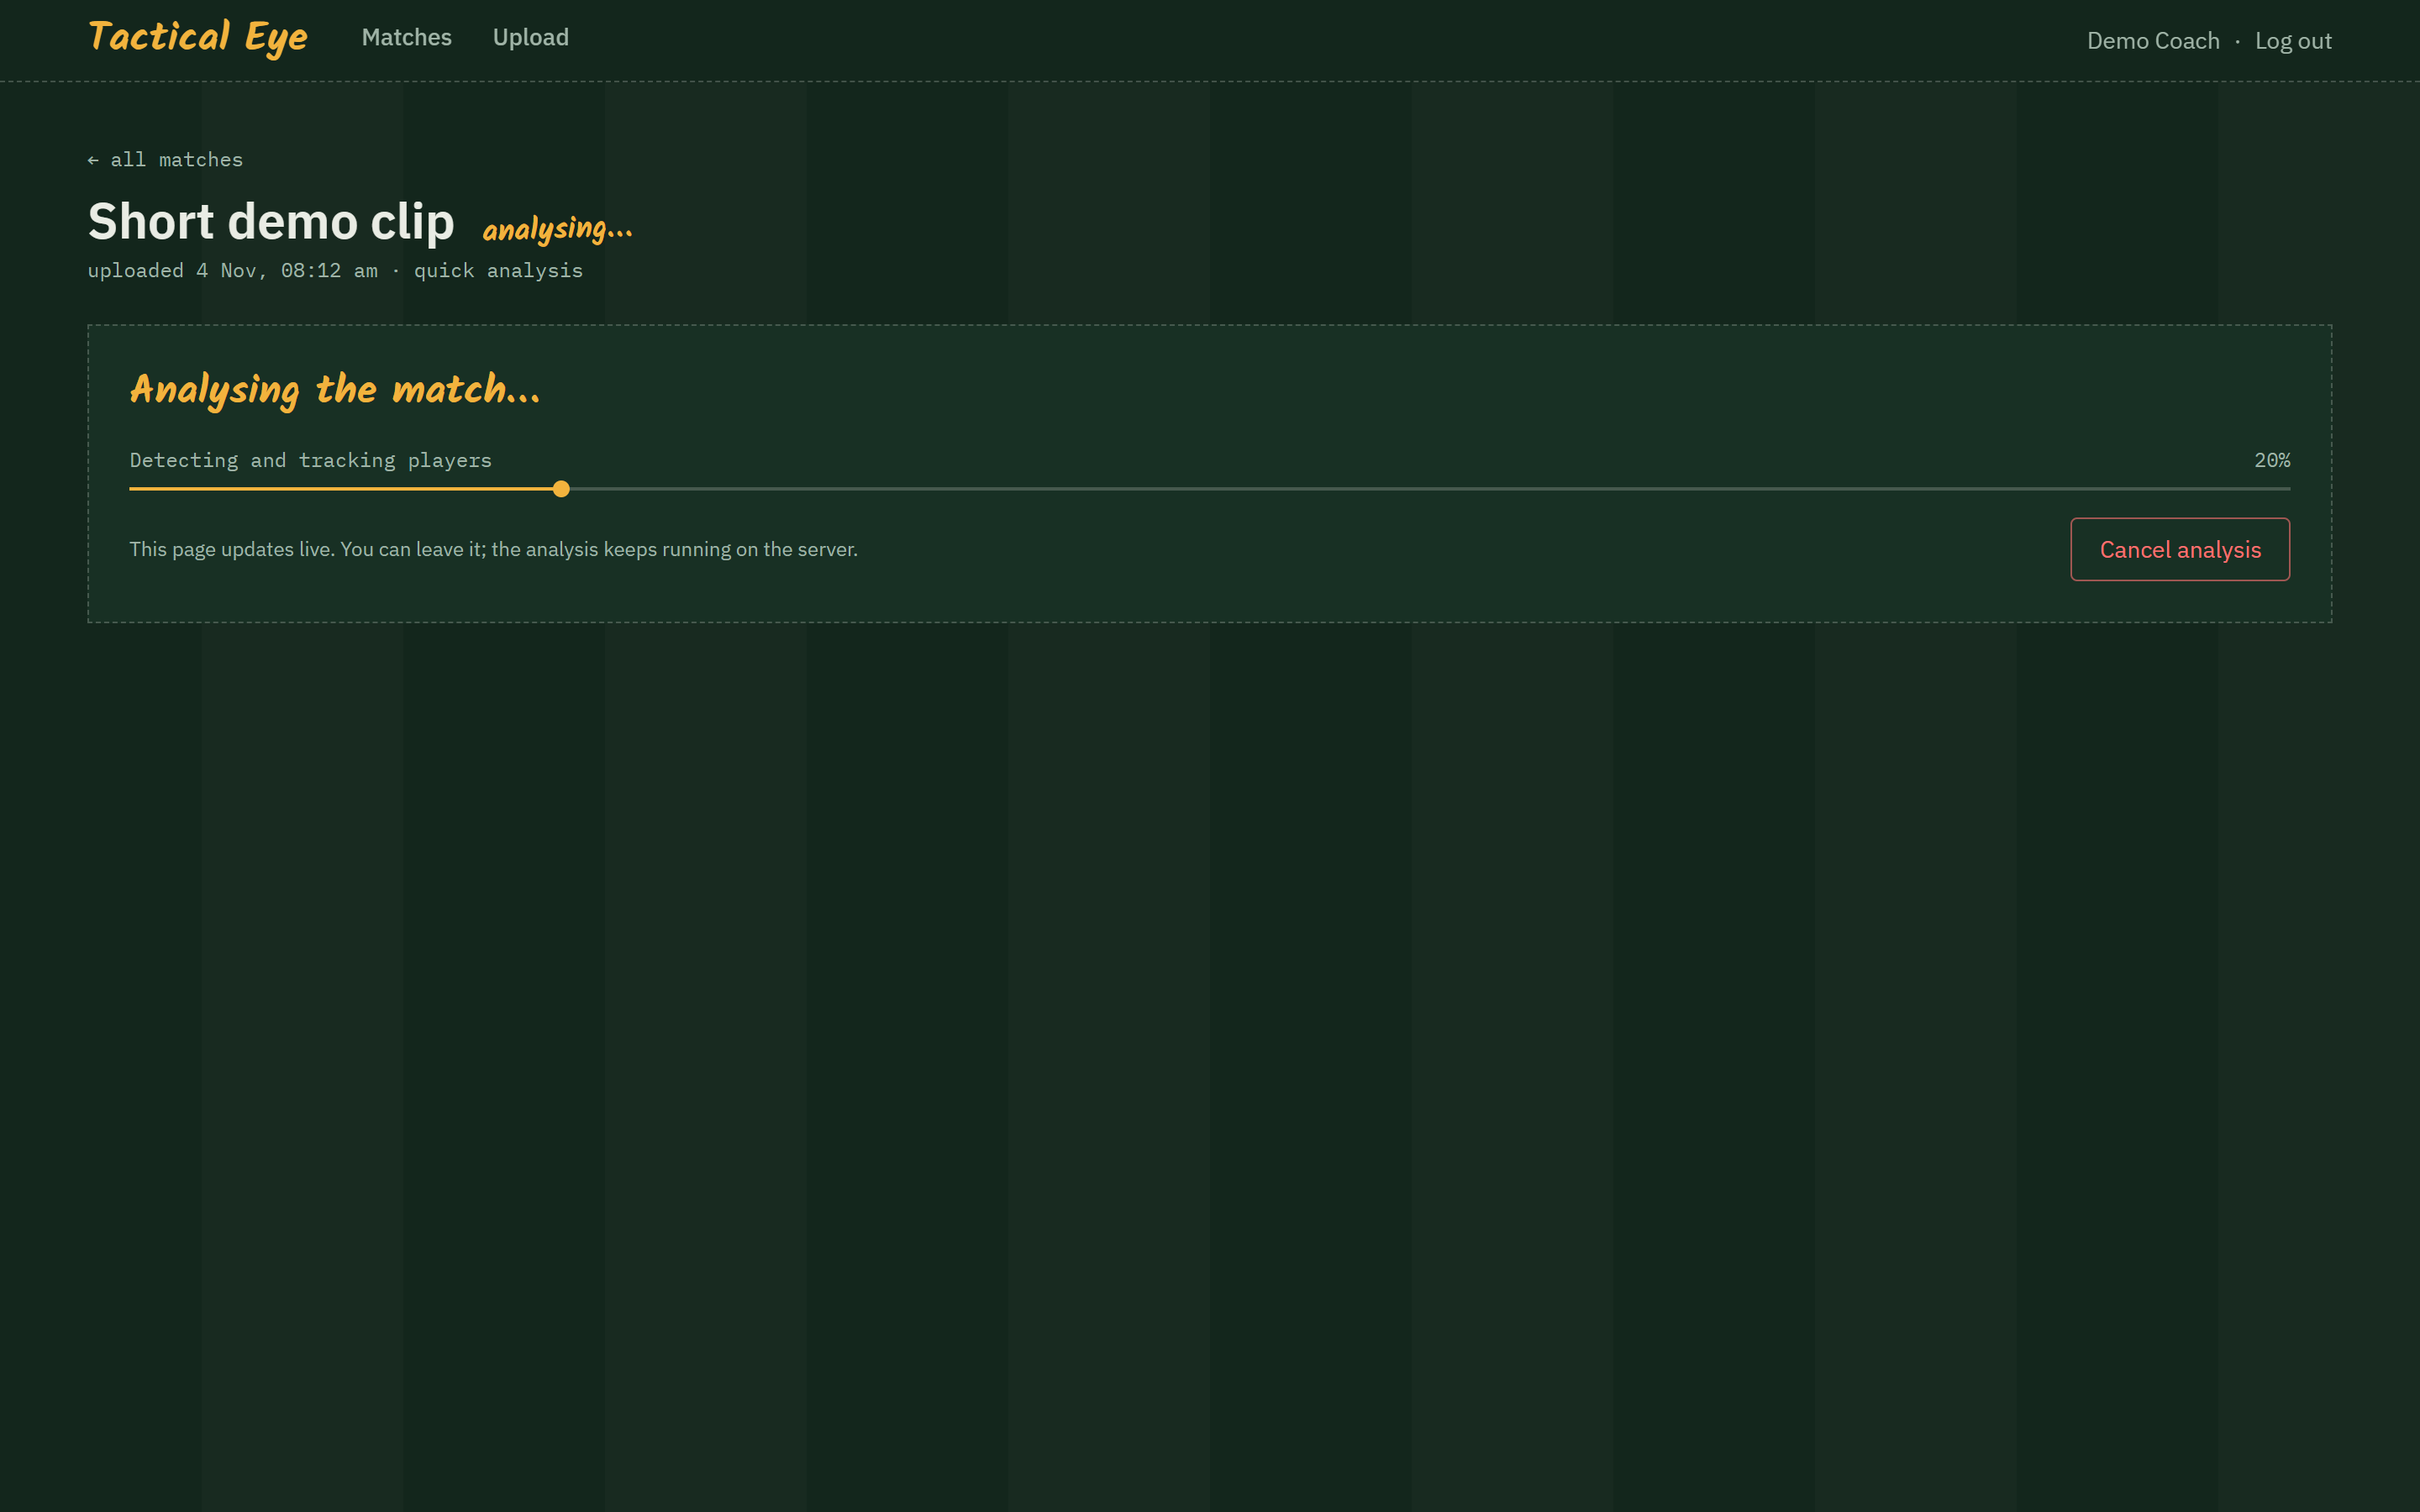
\includegraphics[width=\textwidth]{08_match_in_progress}
	\caption{An analysis in progress, with the \emph{Cancel analysis} button}
	\label{fig:in-progress}
\end{figure}

\begin{figure}[H]
	\centering
	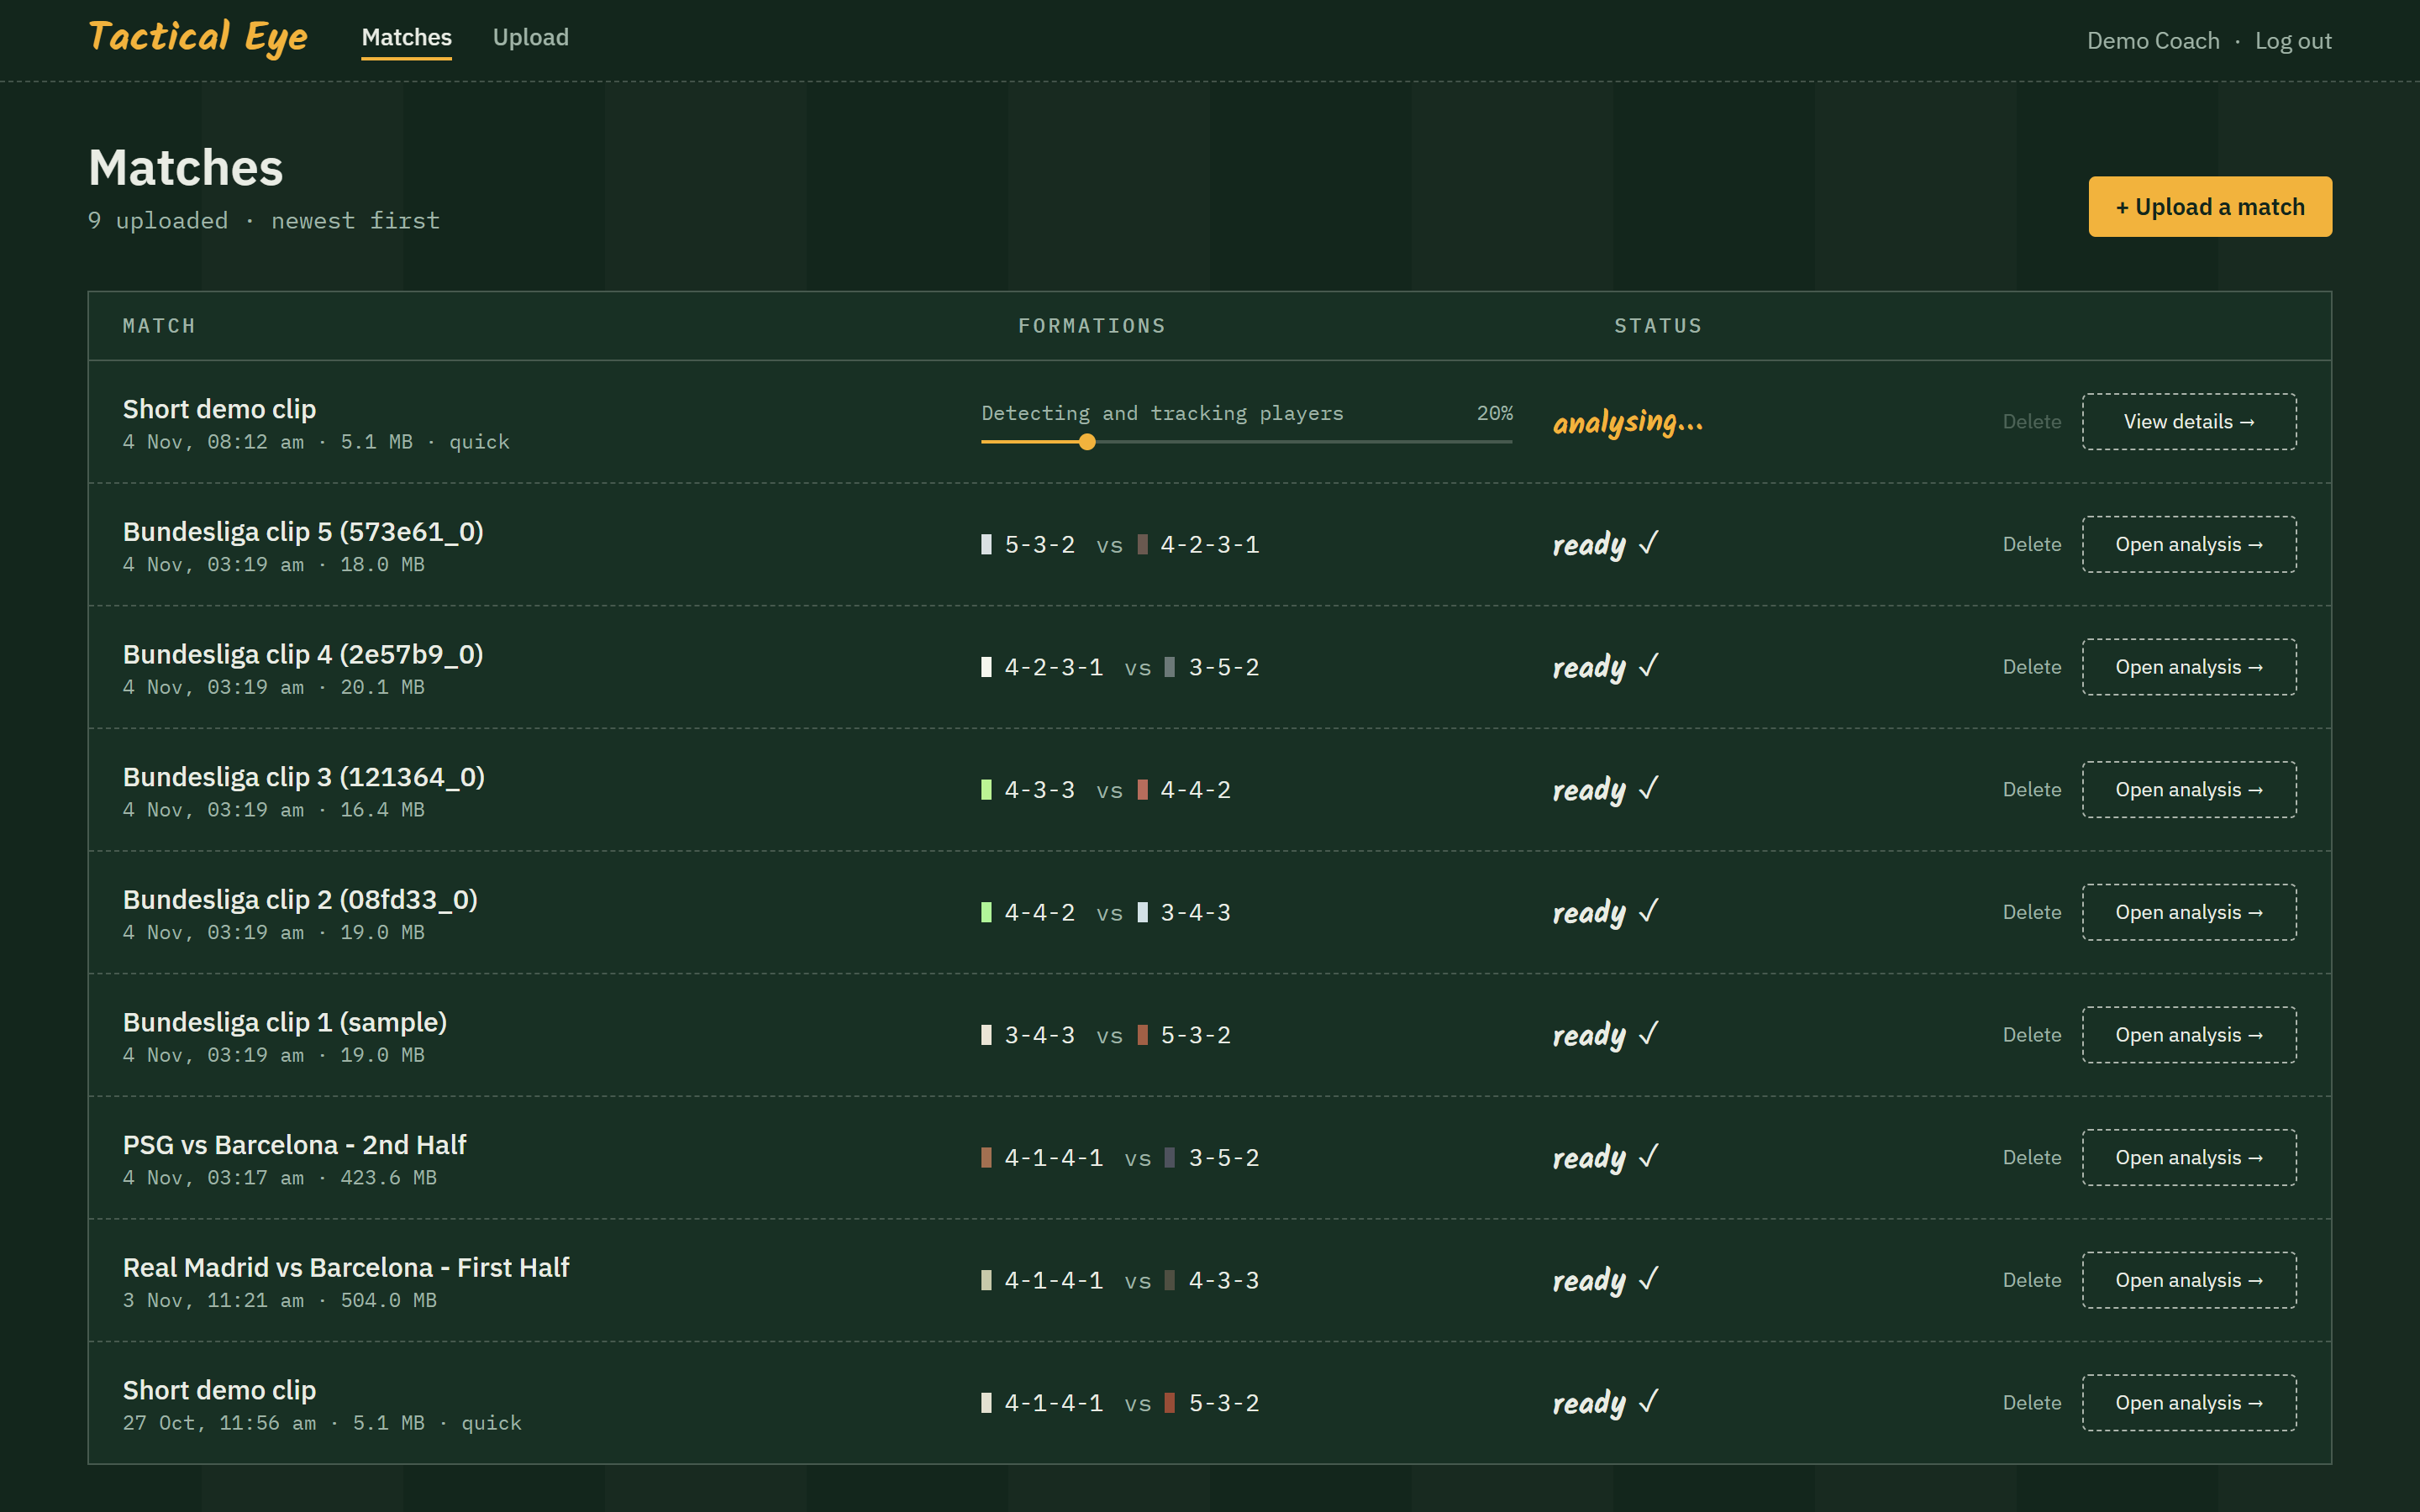
\includegraphics[width=\textwidth]{09_matches_live_progress}
	\caption{Live progress on the match list}
	\label{fig:list-progress}
\end{figure}

\begin{table}[H]
	\centering
	\begin{tabular}{|p{0.34\textwidth}|p{0.10\textwidth}|p{0.48\textwidth}|}
		\hline
		\textbf{Step} & \textbf{Progress} & \textbf{What happens} \\
		\hline
		Uploading video to GPU & 0--5\,\% & Only with the cloud GPU: the video is sent in 50\,MB pieces. \\
		\hline
		Preparing video for playback & 0--5\,\% & A browser-compatible copy of the video is made; the analysis reads this copy. \\
		\hline
		Detecting and tracking players & 5--60\,\% & Every person and the ball are found in each analysed frame and followed through the video. \\
		\hline
		Mapping positions to the pitch & 60--88\,\% & Pitch markings are recognised and positions converted to metres; people off the pitch and false balls are removed. \\
		\hline
		Assigning teams & 88--93\,\% & Players are split into two teams by shirt colour; referees are recognised by their kit. \\
		\hline
		Analysing tactics & 93--98\,\% & Tracks are joined, positions smoothed, formations, position labels and metrics computed. \\
		\hline
		Saving results & 98--100\,\% & The results are stored and the page switches to the analysis view. \\
		\hline
	\end{tabular}
	\caption{The steps shown in the progress bar}
	\label{tab:steps}
\end{table}

If a step fails, the worker tries the whole analysis once more after 10 seconds, and the bar shows \emph{Retrying after an error} in the meantime.

\emph{Cancel analysis} stops an analysis that was started by mistake, for example with the wrong video or in the wrong mode. After a confirmation, a queued analysis is cancelled at once; a running one shows \emph{Cancelling\dots} and stops within a few seconds, also on the cloud GPU. The match then shows the note in \autoref{fig:cancelled} and can be started again with \emph{Re-analyse}. Cancelling a \emph{re-analysis} of a finished match does not lose anything: the match simply goes back to its earlier results.

\begin{figure}[H]
	\centering
	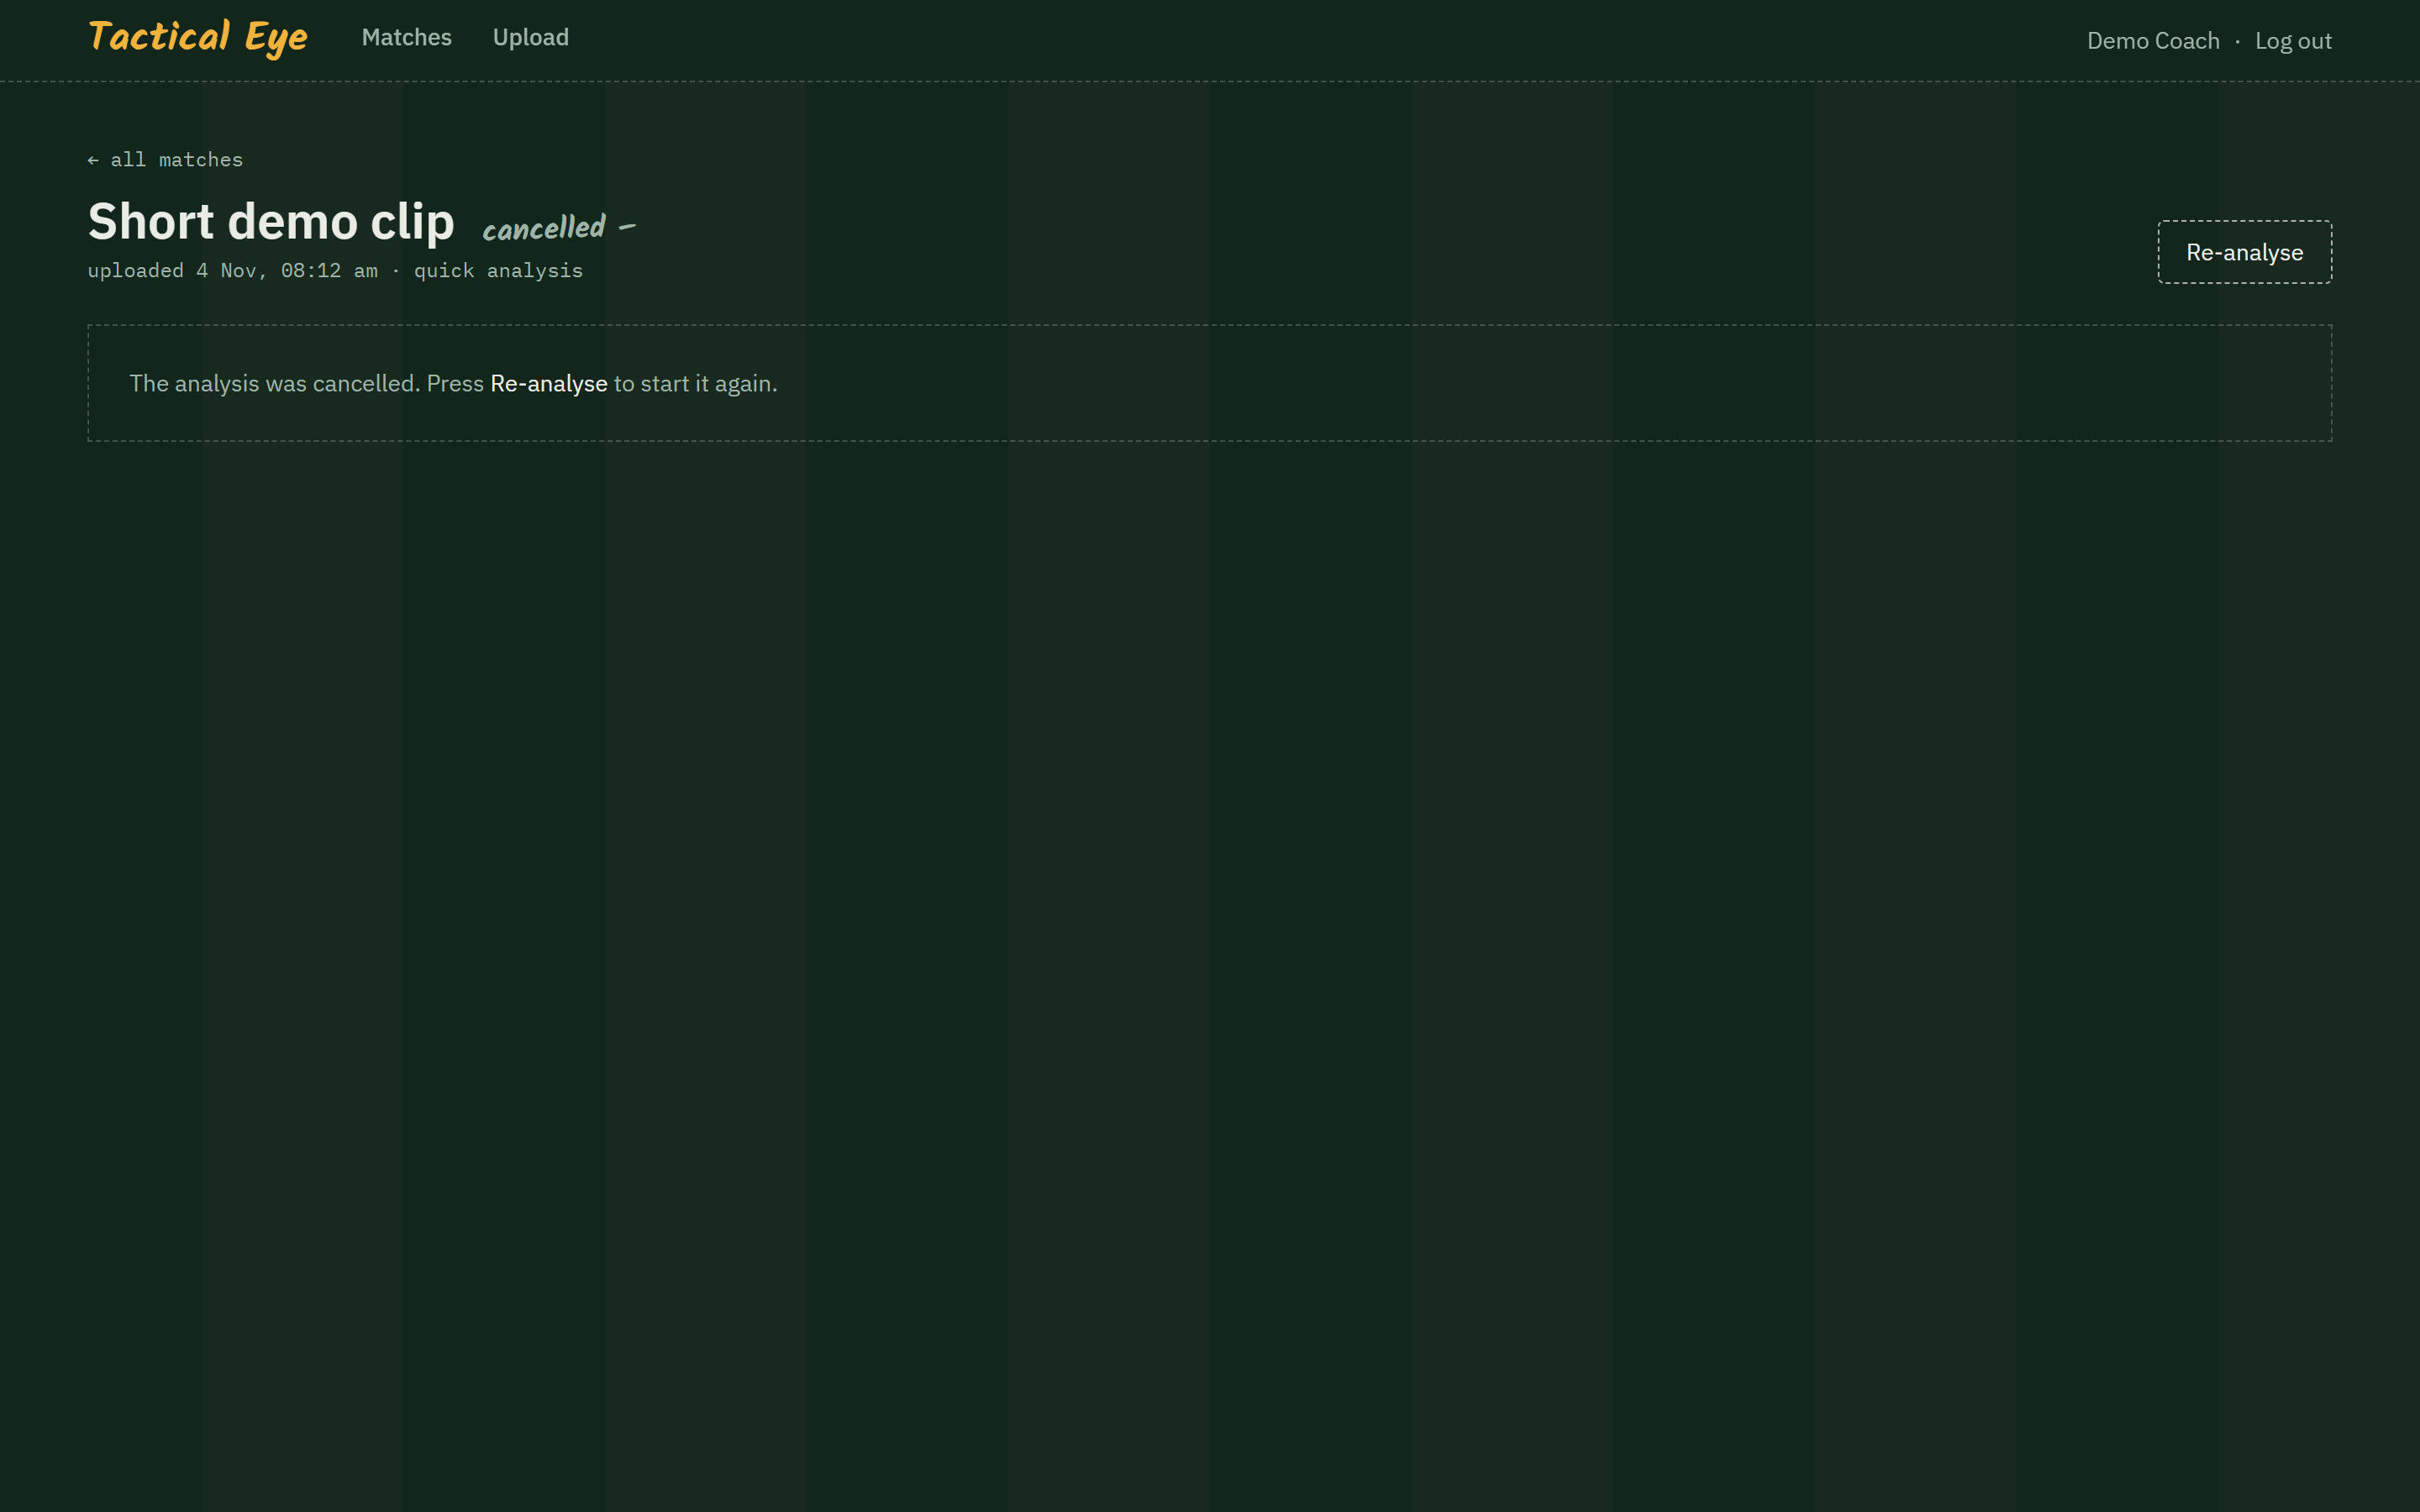
\includegraphics[width=\textwidth]{10_match_cancelled}
	\caption{A cancelled analysis}
	\label{fig:cancelled}
\end{figure}

\section{The analysis page}

When the analysis has finished, the match page shows the interactive analysis (\autoref{fig:intro-analysis} on page~\pageref{fig:intro-analysis}). Under the title, one line tells when the match was uploaded, in which mode it was analysed, and where and how long the processing took. The page has four parts: the video with its overlays and controls on the left, the tactical board with the current formations on the right, the layer buttons under the video, and three tabs further down with the summary, the selected player and the AI coaching report. \emph{Re-analyse} in the top right corner and \emph{$\leftarrow$ all matches} are described in \autoref{sec:reanalyse-delete}.

\subsection{Video player and controls}

The video plays inside the page. The browser's own controls are replaced by the controls under the video (\autoref{tab:video-controls}), because the drawings cover the video surface.

\begin{table}[H]
	\centering
	\begin{tabular}{|p{0.24\textwidth}|p{0.68\textwidth}|}
		\hline
		\textbf{Control} & \textbf{Action} \\
		\hline
		play / pause & Starts or pauses playback. Clicking an empty spot of the video does the same. \\
		\hline
		$\blacktriangleleft$ 1f / 1f $\blacktriangleright$ & Pauses and steps exactly one frame back or forward, for studying a situation. \\
		\hline
		Seek bar & Jumps to any moment; the time is shown as minutes:seconds.tenths. \\
		\hline
		Speed (1$\times$, 0.5$\times$, 0.25$\times$) & Slows playback down; the drawings stay in sync at every speed. \\
		\hline
		Full-screen button & In the bottom-right corner of the video. Shows the video, its drawings, the controls and the layer buttons on the whole screen (\autoref{fig:fullscreen}); the same button or Esc leaves full screen. \\
		\hline
	\end{tabular}
	\caption{Video controls}
	\label{tab:video-controls}
\end{table}

\begin{figure}[H]
	\centering
	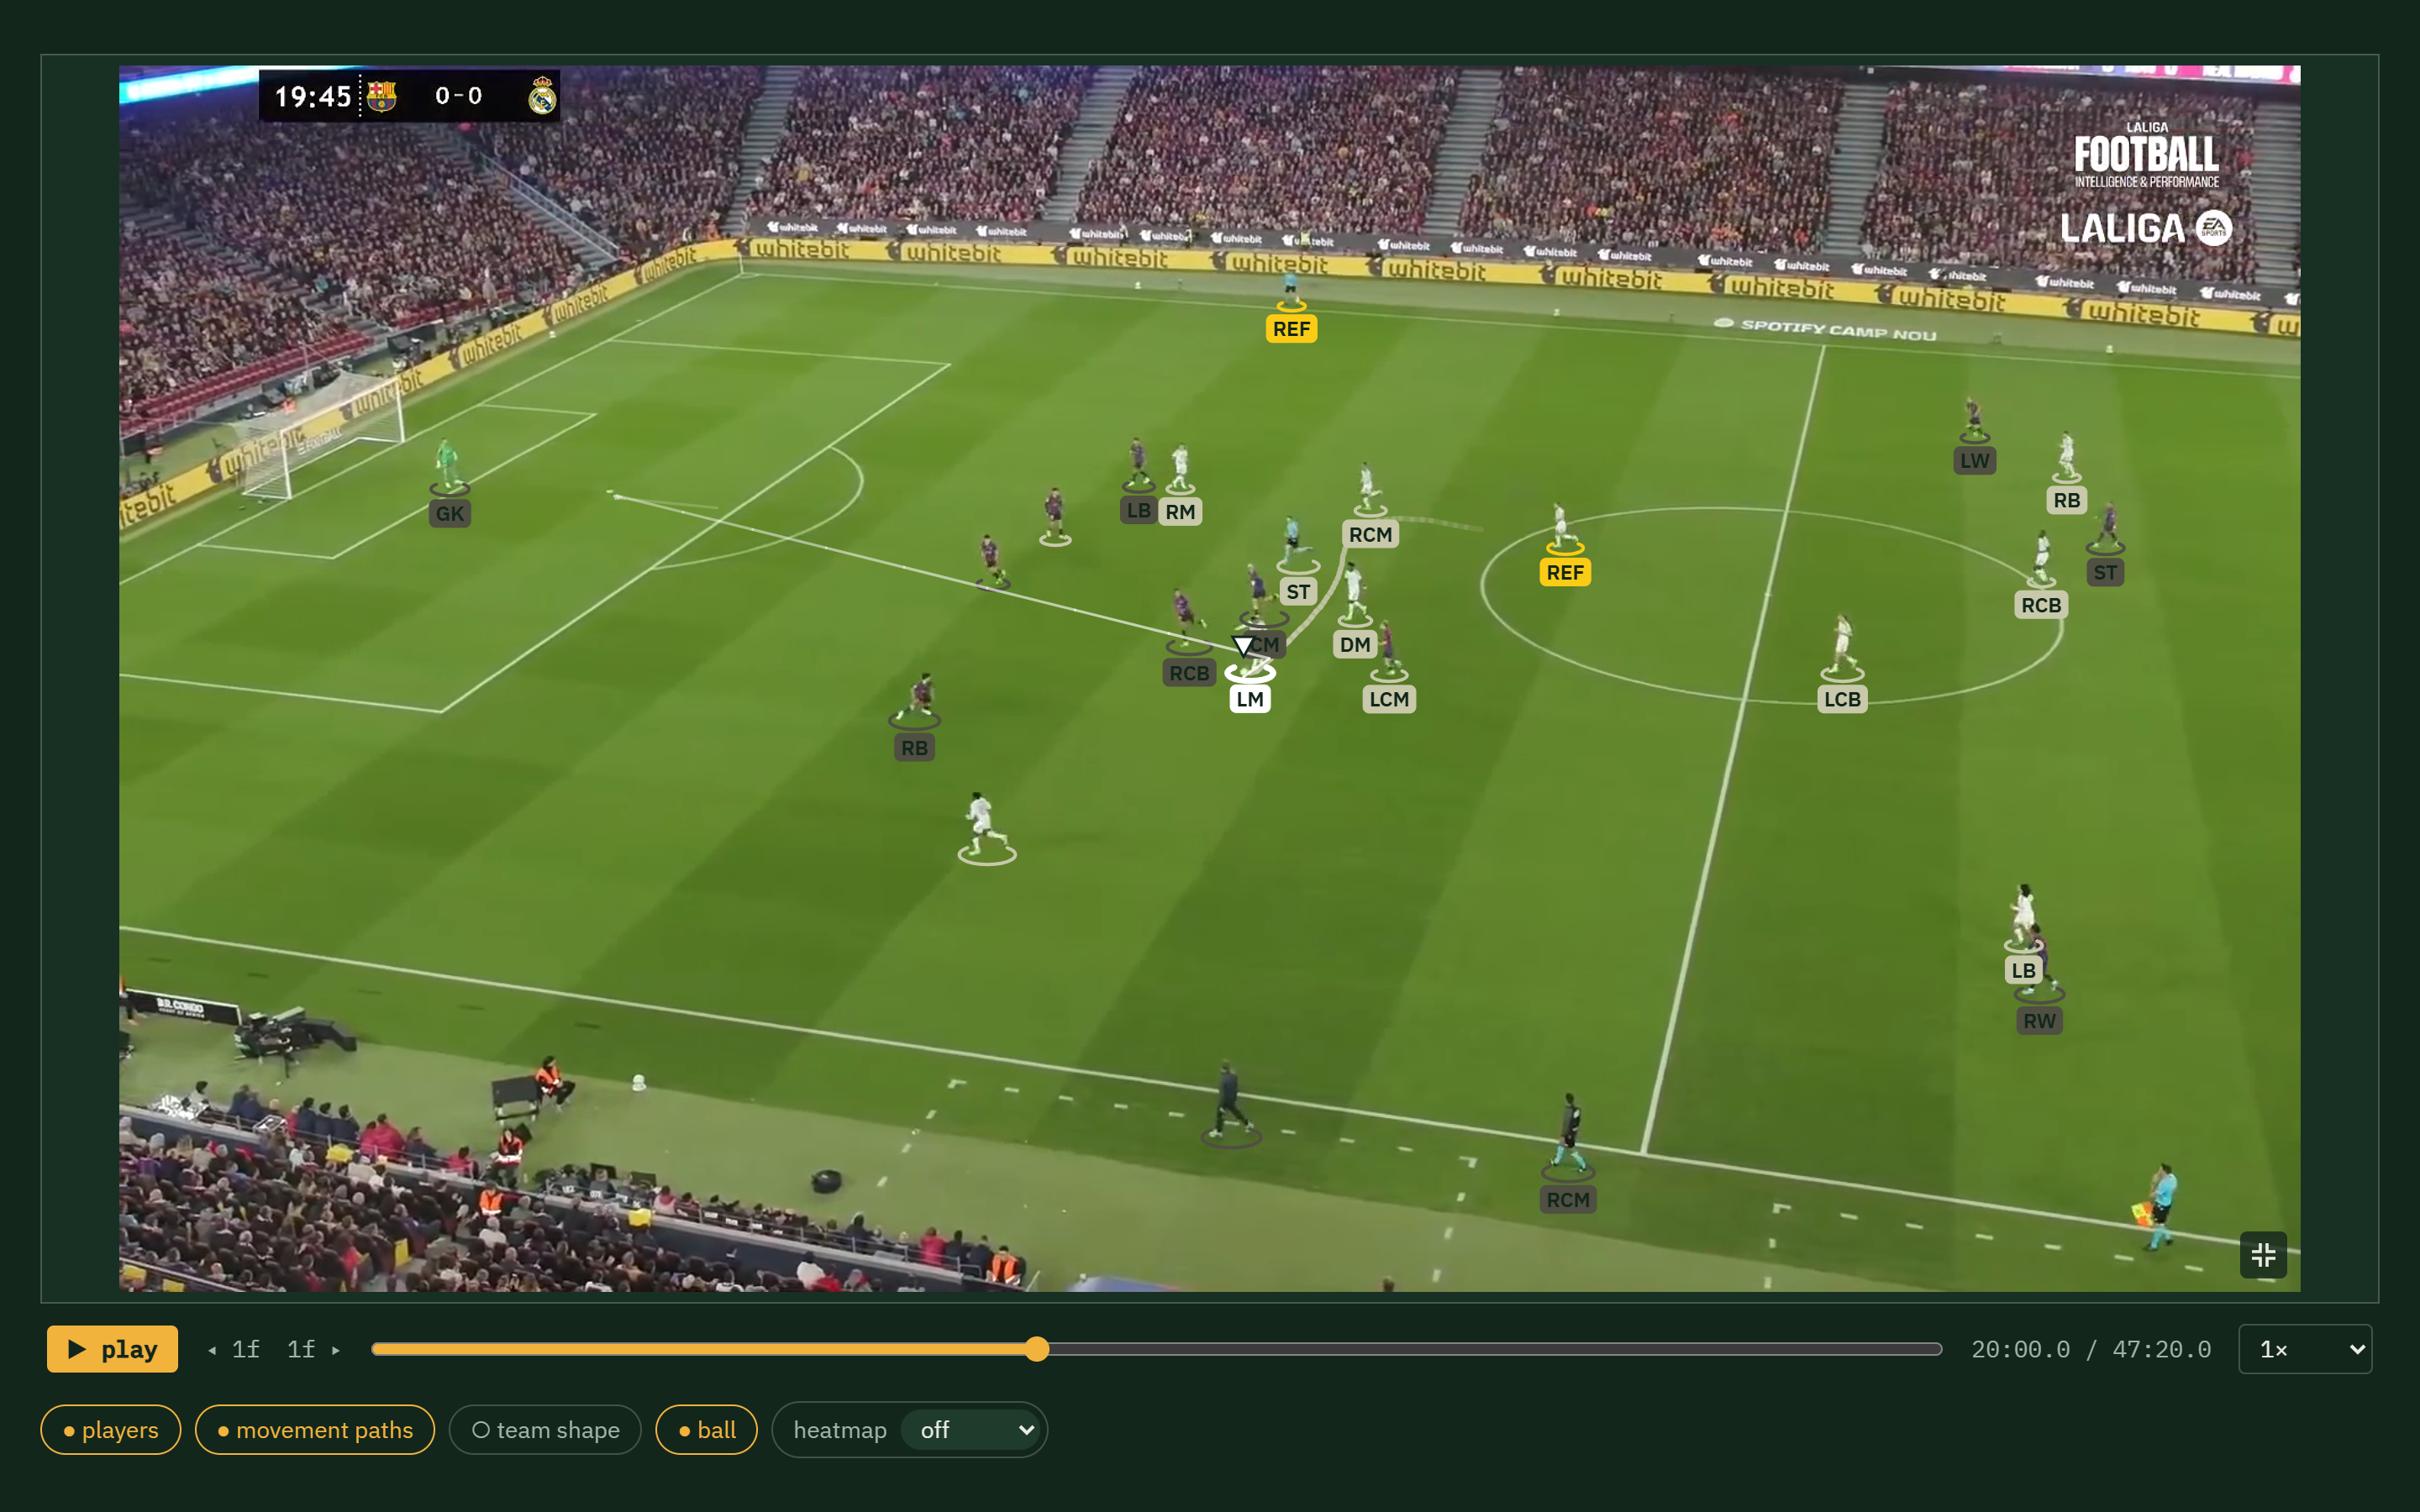
\includegraphics[width=\textwidth]{22_full_screen}
	\caption{Full-screen mode}
	\label{fig:fullscreen}
\end{figure}

All drawings follow the video frame by frame, also while the camera pans and zooms, because they are re-projected through the camera geometry of every frame (\autoref{sec:overlay-sync}).

\subsection{Overlay layers}

The layer buttons (\autoref{fig:layers}) switch the drawings on the video and on the board on and off; a filled dot means the layer is visible. \autoref{tab:layers} describes them.

\begin{figure}[H]
	\centering
	
\includegraphics[width=0.85\textwidth]{16_layer_controls}
	\caption{The layer buttons}
	\label{fig:layers}
\end{figure}

\begin{table}[H]
	\centering
	\begin{tabular}{|p{0.20\textwidth}|p{0.72\textwidth}|}
		\hline
		\textbf{Layer} & \textbf{What is drawn} \\
		\hline
		players & An ellipse at each person's feet in their kit colour with a label: the position (LB, RCB, DM, ST\dots) for players, GK for goalkeepers and REF for referees, in yellow. A player whose position is unknown at that moment gets only the ellipse. \\
		\hline
		movement paths & The path of the last 4 seconds, drawn on the grass and fading with age (\autoref{fig:paths}). When a player is selected, only their path is shown. \\
		\hline
		team shape & The area enclosed by each team's outfield players, filled in the team colour (\autoref{fig:shape}). A small area means a compact team. \\
		\hline
		ball & A marker above the ball and its path over the last 1.5 seconds. \\
		\hline
		heatmap (menu) & Off, Team A, Team B or Ball: where that team's players, or the ball, spent the most time over the whole video, from rarely (blue-green) to most often (red), painted onto the pitch (\autoref{fig:heatmaps}). \\
		\hline
	\end{tabular}
	\caption{Overlay layers}
	\label{tab:layers}
\end{table}

\begin{figure}[H]
	\centering
	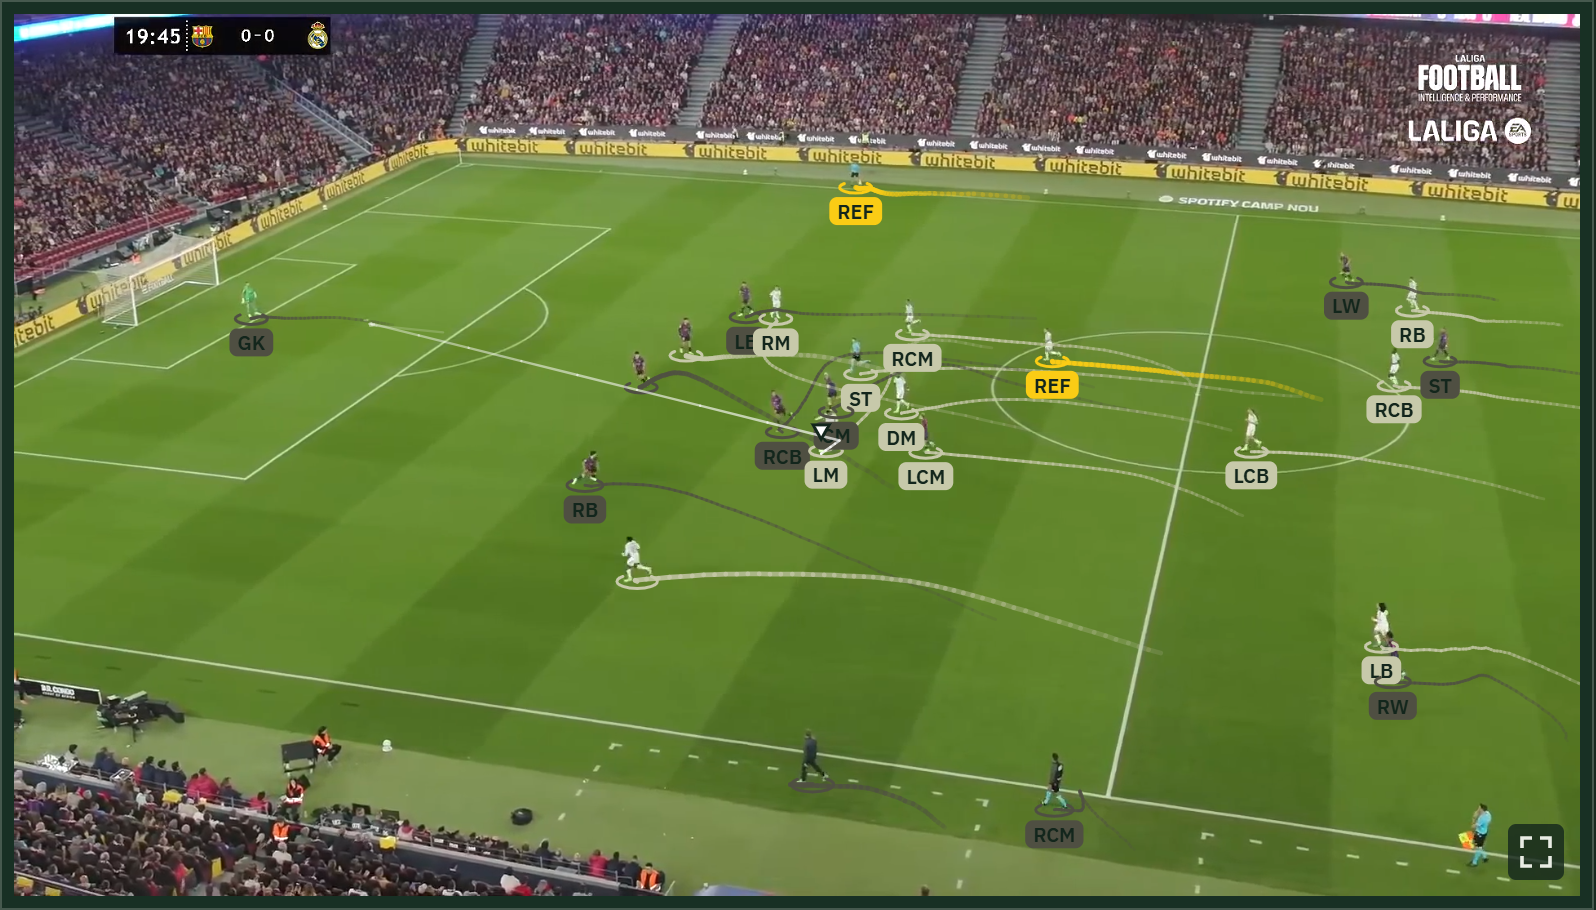
\includegraphics[width=\textwidth]{12_overlay_players_paths}
	\caption{Position labels and movement paths drawn on the video; the referees are labelled REF}
	\label{fig:paths}
\end{figure}

\begin{figure}[H]
	\centering
	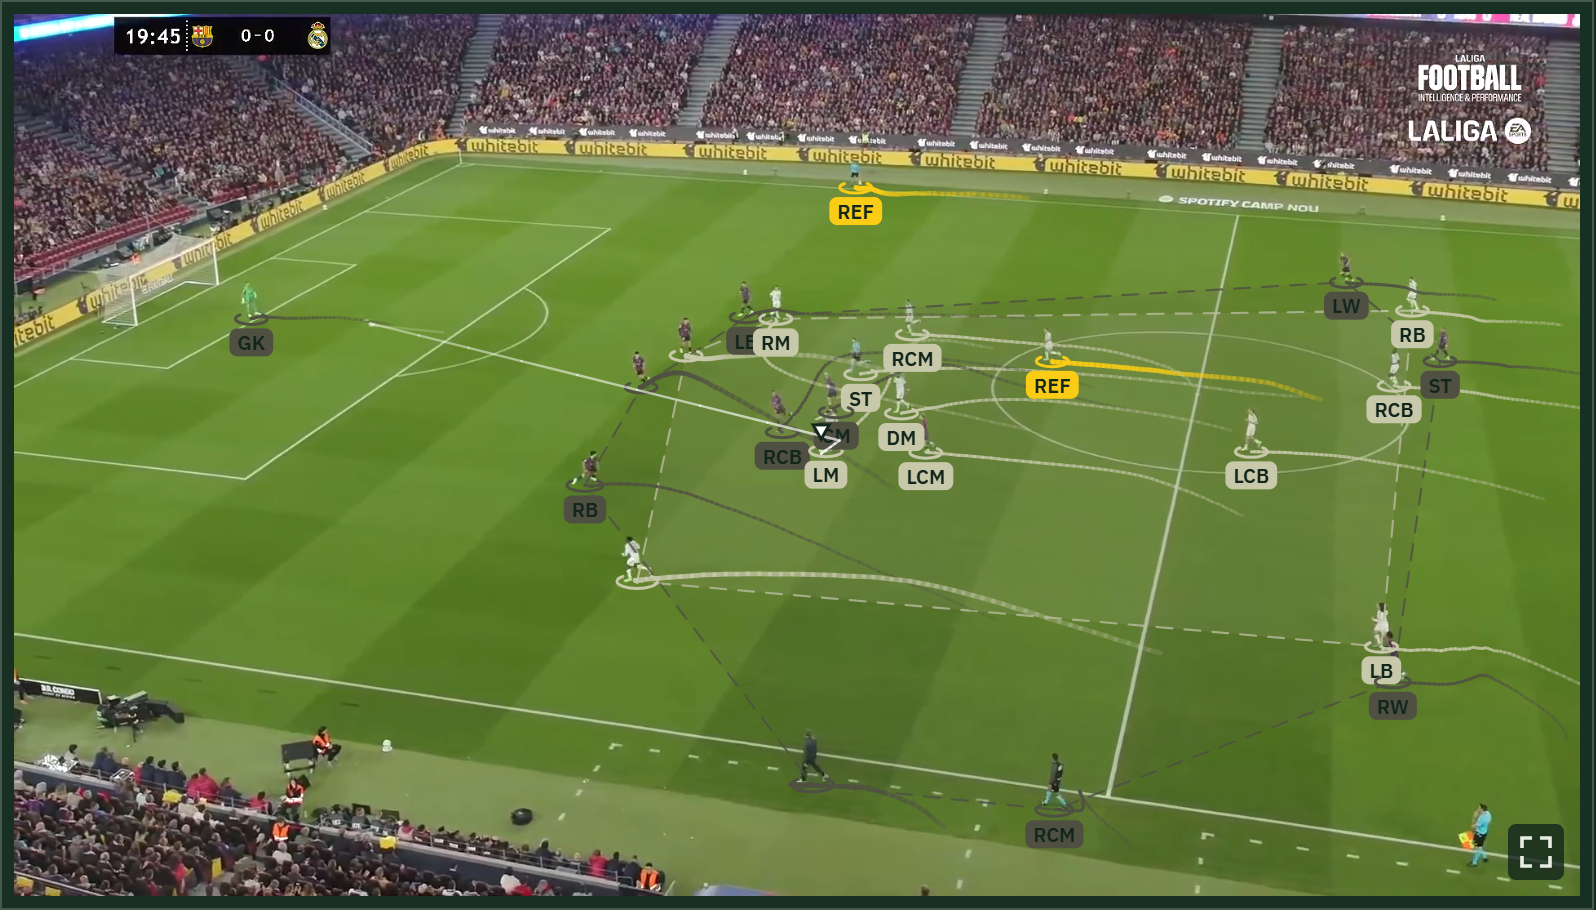
\includegraphics[width=\textwidth]{13_overlay_team_shape}
	\caption{The team shape layer}
	\label{fig:shape}
\end{figure}

\begin{figure}[H]
	\centering
	\begin{subfigure}{0.49\textwidth}
		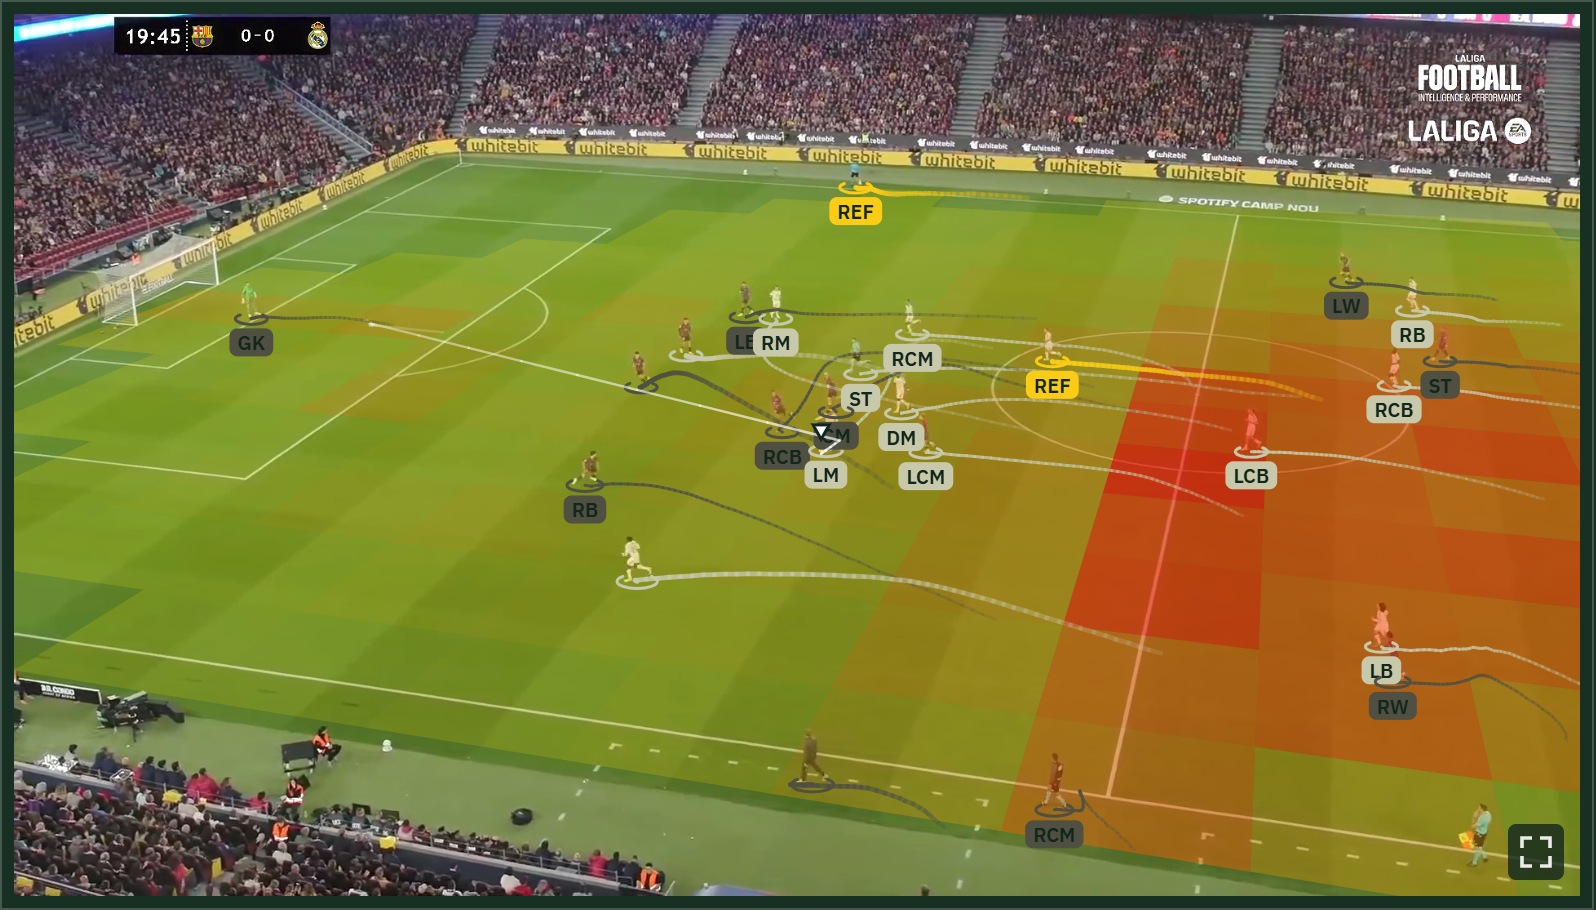
\includegraphics[width=\textwidth]{14_overlay_heatmap_team_a}
		\caption{Team A}
	\end{subfigure}
	\hfill
	\begin{subfigure}{0.49\textwidth}
		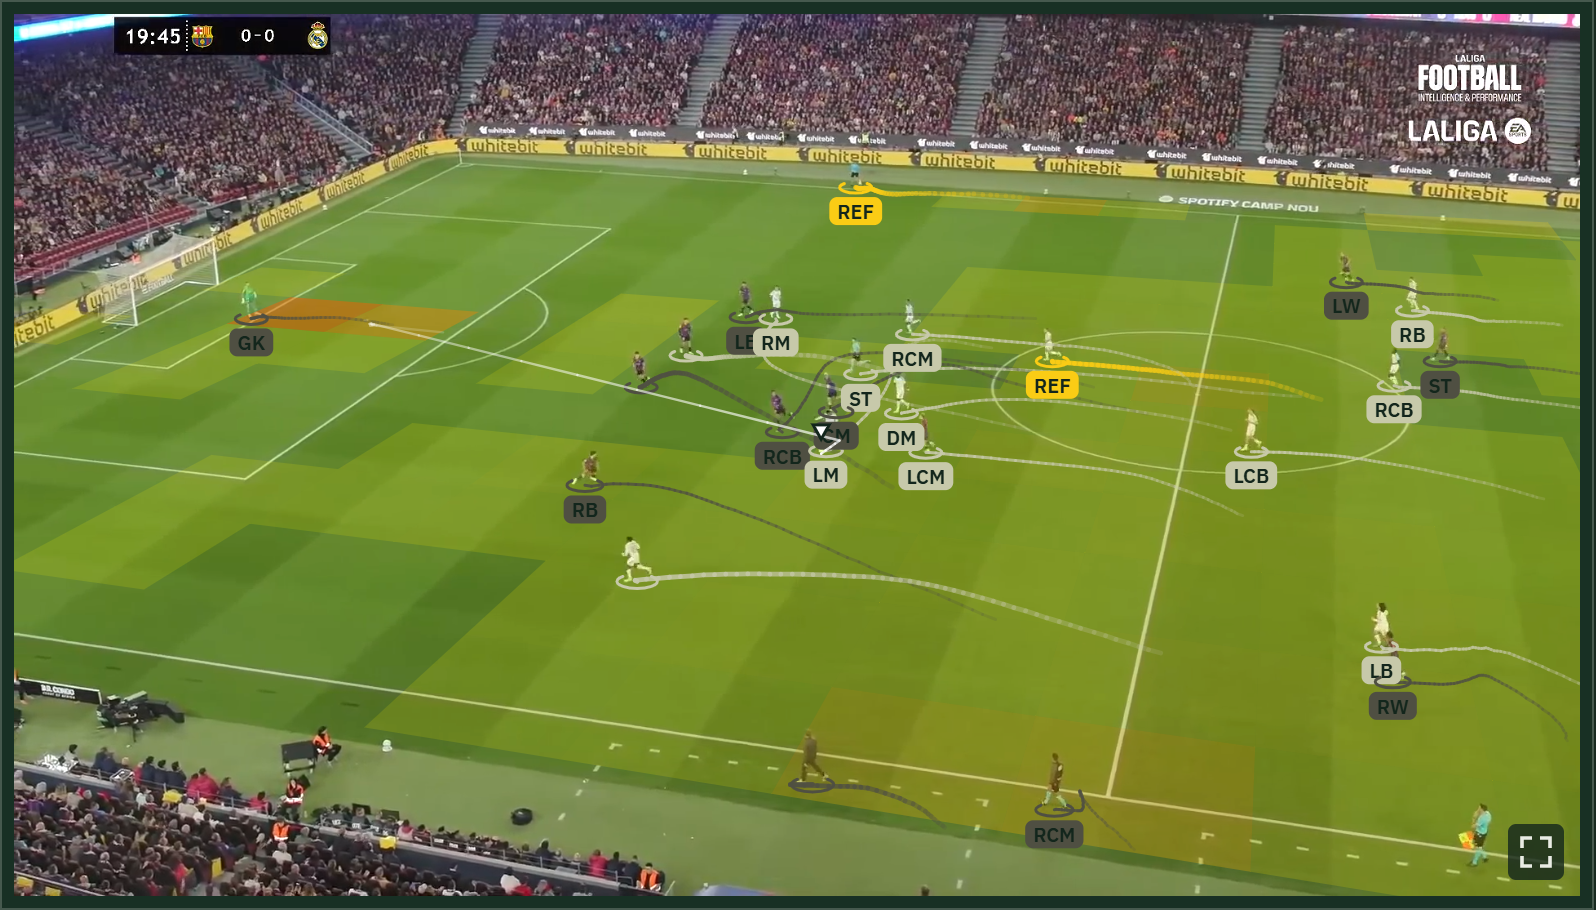
\includegraphics[width=\textwidth]{15_overlay_heatmap_ball}
		\caption{Ball}
	\end{subfigure}
	\caption{Heatmaps painted onto the pitch in the video}
	\label{fig:heatmaps}
\end{figure}

\subsection{Tactical board and formations}

The tactical board (\autoref{fig:board}) shows the same moment as the video from above, on a to-scale $105 \times 68$\,m pitch drawn like a chalkboard: Team A as circles, Team B as crosses, referees as small yellow squares and the ball as a white dot, each player with their position label. The board uses the same layers as the video. Unlike the video, it shows true metric proportions, so distances and spacing are easy to judge.

Under the board, two cards show the formation each team plays at the current moment, for example 3-4-3 and 4-2-3-1, with the runner-up, the second best fitting formation. A close runner-up means that the team's shape lies between two formations. Formations are worked out in 5-second windows, and a new one is only accepted once it has lasted about 20 seconds, so short wobbles do not count as changes.

\begin{figure}[H]
	\centering
	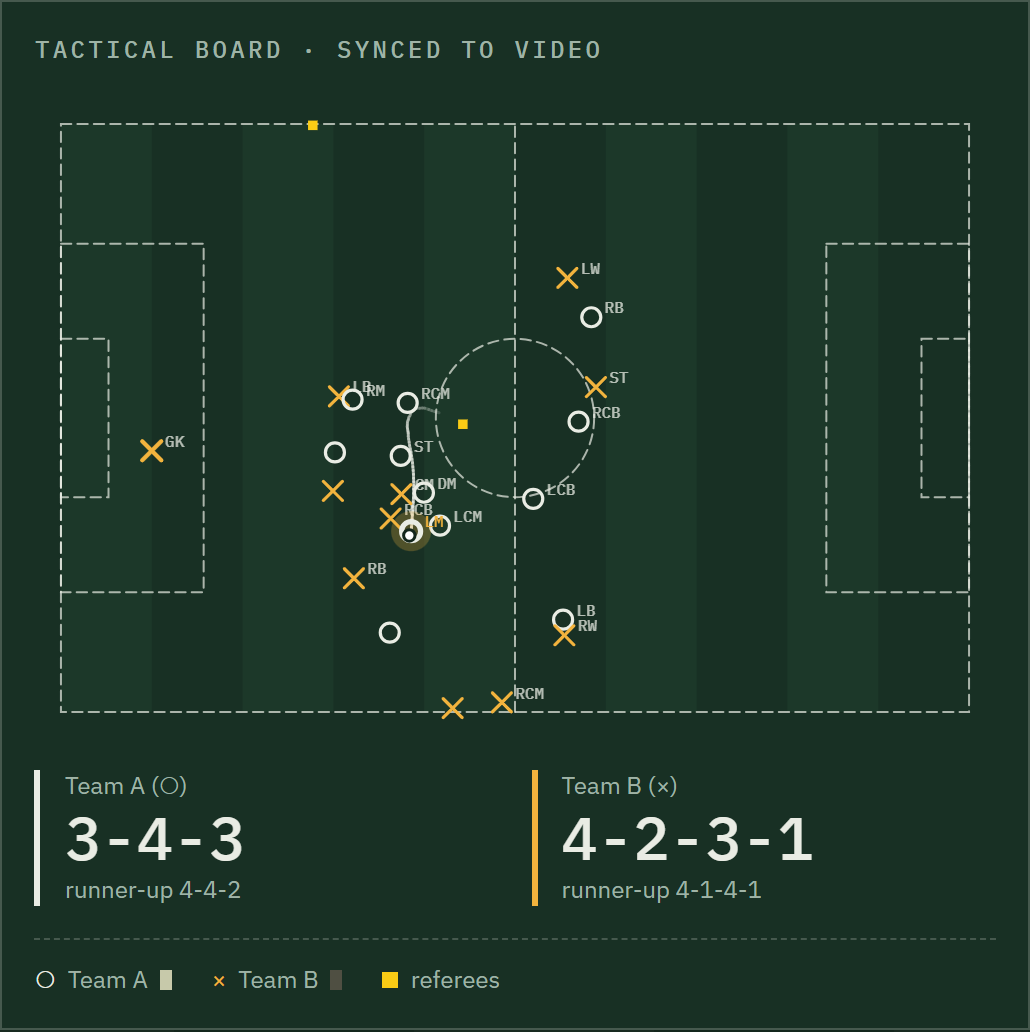
\includegraphics[width=0.6\textwidth]{18_board_and_formations}
	\caption{The tactical board with the current formations and the legend}
	\label{fig:board}
\end{figure}

\subsection{Inspecting a position}

Clicking a player on the video or on the board selects them: their marker is highlighted, their path is shown, and the \emph{Player} tab opens with the name of the position, for example ``Team A $\cdot$ LM'' (\autoref{fig:player-panel}). The tab shows a small pitch with the heatmap and the path of that position over the whole video, the distance covered, the time visible, the average speed and the top speed. The top speed is the best average over one second, not the fastest single step, which would be distorted by measurement noise (\autoref{sec:metrics}).

These numbers belong to the \emph{position}, not to a named player. One broadcast camera cannot follow the same player through a whole match (\autoref{sec:positions}), so the left back's statistics cover whoever played left back while visible. Clicking the same player again, or \emph{clear selection}, removes the selection.

\begin{figure}[H]
	\centering
	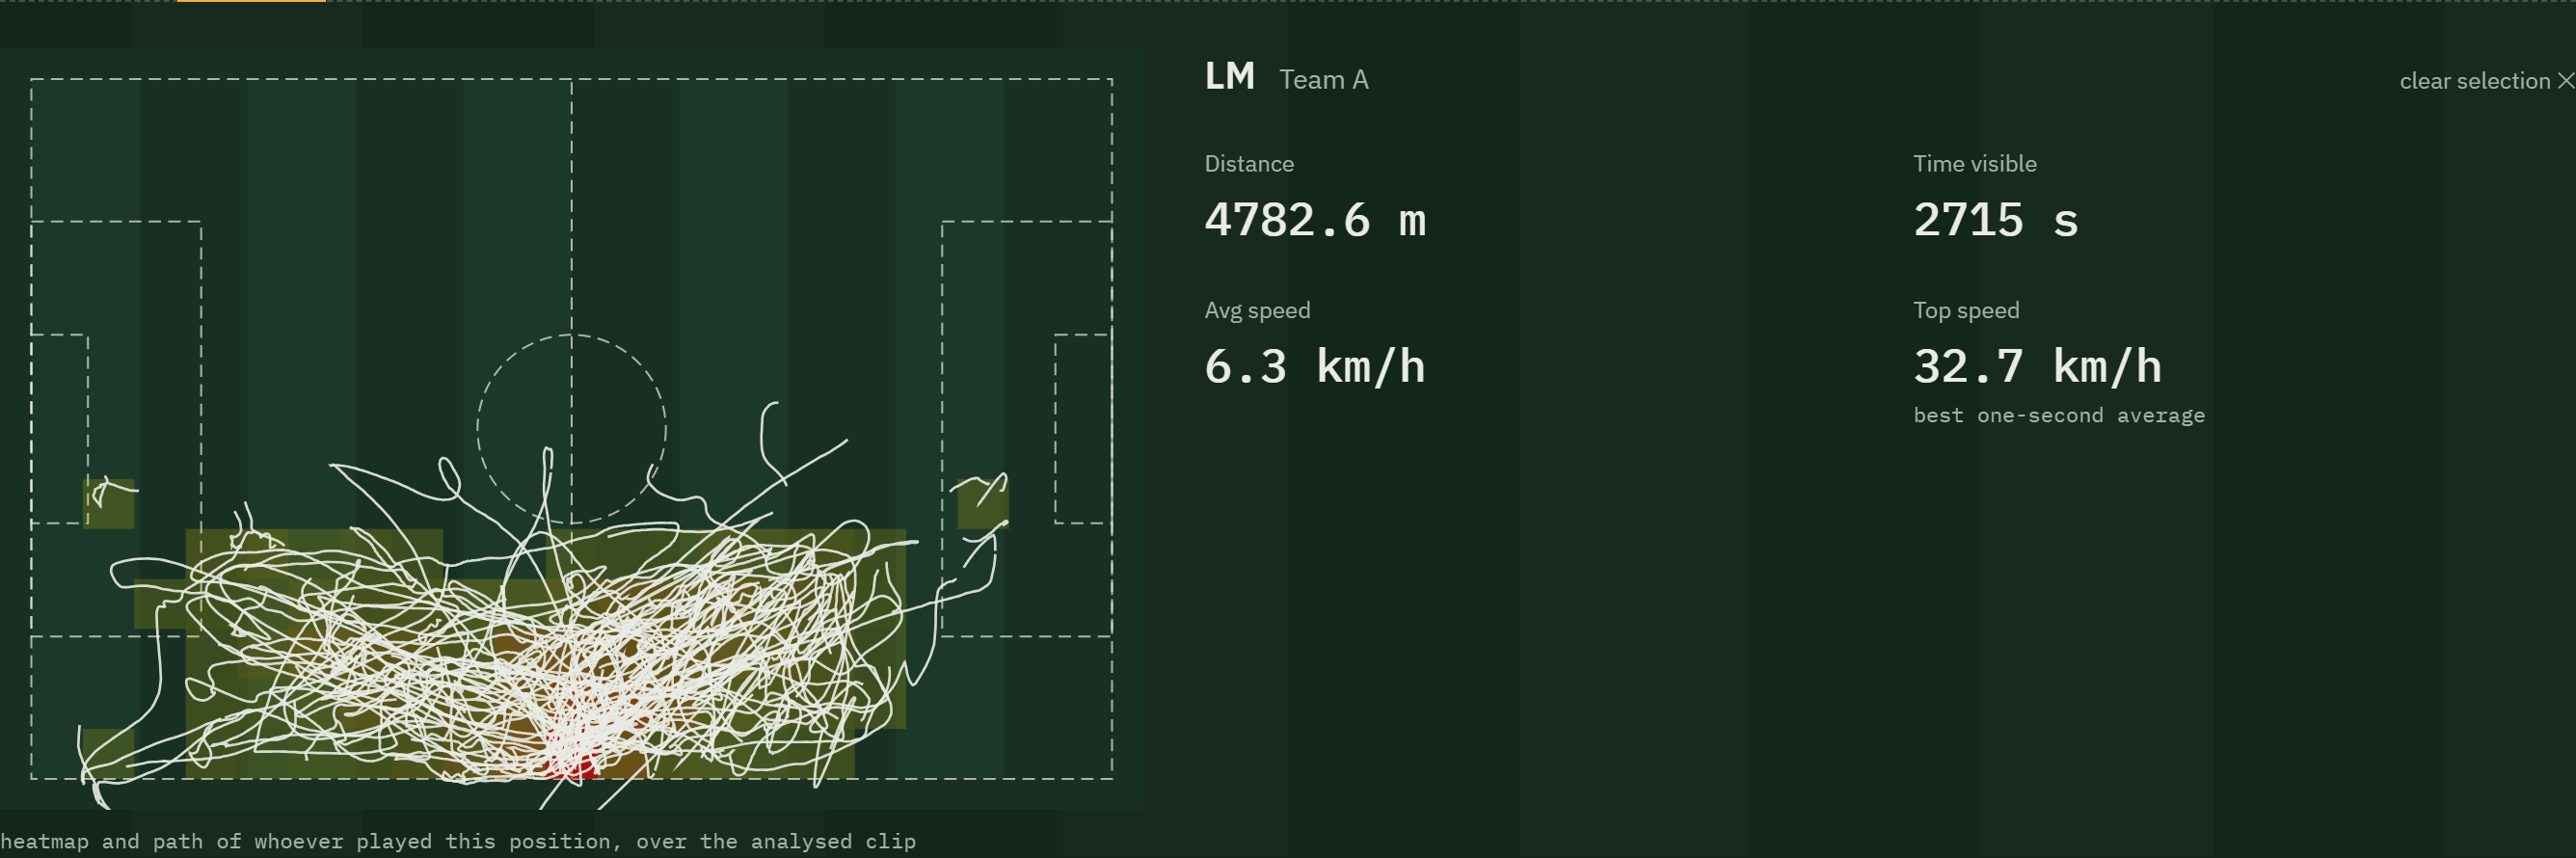
\includegraphics[width=\textwidth]{19_player_panel}
	\caption{The \emph{Player} tab of the left midfielder (LM) of Team A over a full half}
	\label{fig:player-panel}
\end{figure}

\subsection{Summary}

The \emph{Summary} tab (\autoref{fig:summary}) compares the two teams side by side. \autoref{tab:summary-metrics} explains the rows. Under the table, four numbers describe the video: its length, the number of frames analysed, the share of analysed frames in which the ball was found, and the number of formation changes.

\begin{figure}[H]
	\centering
	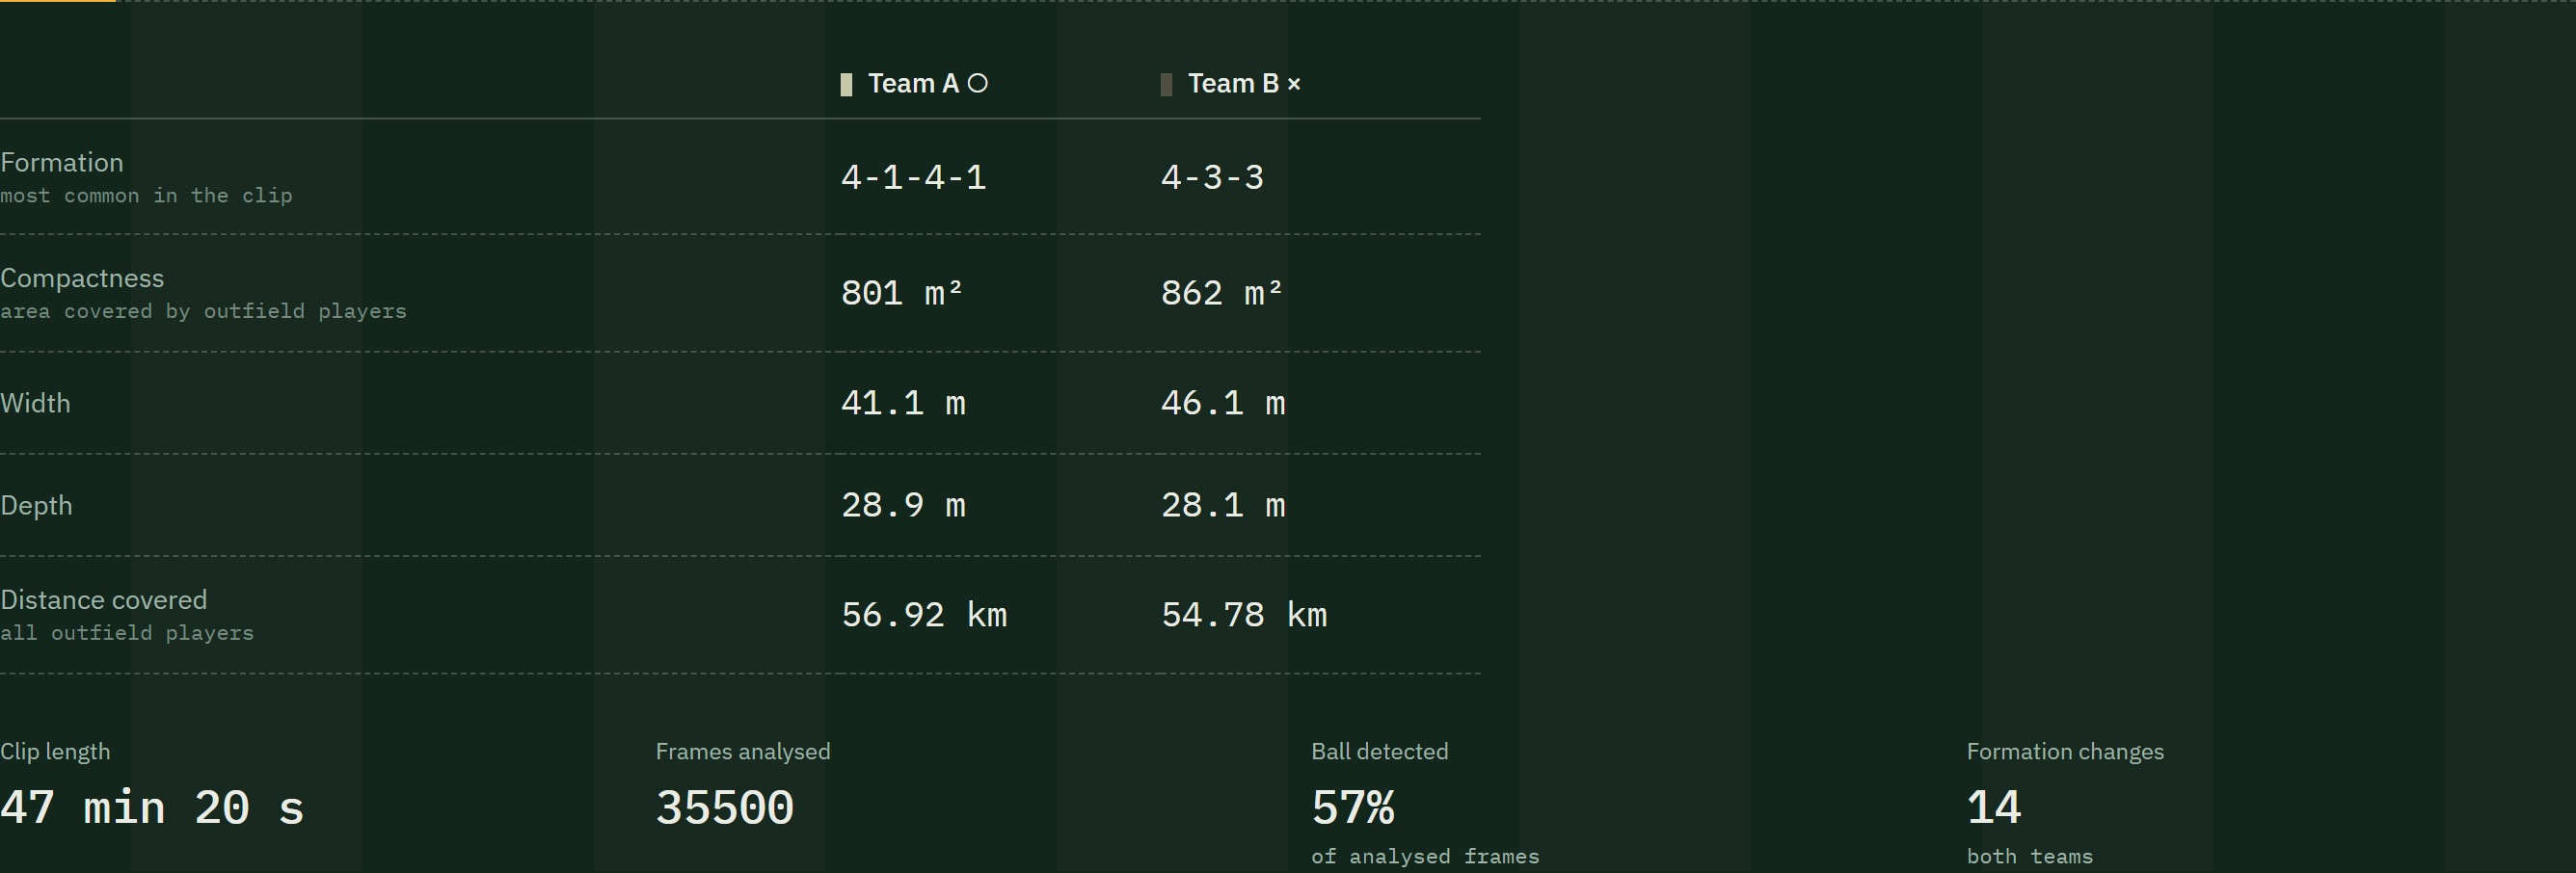
\includegraphics[width=\textwidth]{20_summary}
	\caption{The summary of the first half}
	\label{fig:summary}
\end{figure}

\begin{table}[H]
	\centering
	\begin{tabular}{|p{0.22\textwidth}|p{0.70\textwidth}|}
		\hline
		\textbf{Row} & \textbf{Meaning} \\
		\hline
		Formation & The team's most frequent formation in the video. \\
		\hline
		Compactness & Average area (m\textsuperscript{2}) enclosed by the outfield players. Smaller means the team stays closer together, typical of defending. \\
		\hline
		Width & Average distance (m) between the team's outermost players across the pitch. \\
		\hline
		Depth & Average distance (m) between the team's deepest and most advanced players. \\
		\hline
		Distance covered & Total distance run by the outfield players while visible, in km. \\
		\hline
	\end{tabular}
	\caption{Team metrics in the summary}
	\label{tab:summary-metrics}
\end{table}

\subsection{AI coaching report}

The \emph{AI coaching report} tab turns the statistics into a short written analysis (\autoref{fig:report}). \emph{Generate report} produces it in about 10--30 seconds, with the sections Overview, Team A, Team B, Shape over time, Recommendations and Data limitations. The report is stored with the match and shown at once the next time; \emph{Regenerate} writes a new version.

The report names the teams by their kit colour, such as ``Team A (white)'', and players by their position, such as the left back (LB). It is based only on the measured numbers: formations over time, compactness, width and depth in each third of the video, and the positions that ran the furthest. It is told not to invent events that are not measured, such as passes or goals, and to state the limits of the data. It is a starting point for the coach's own analysis, not a replacement for it.

\begin{figure}[H]
	\centering
	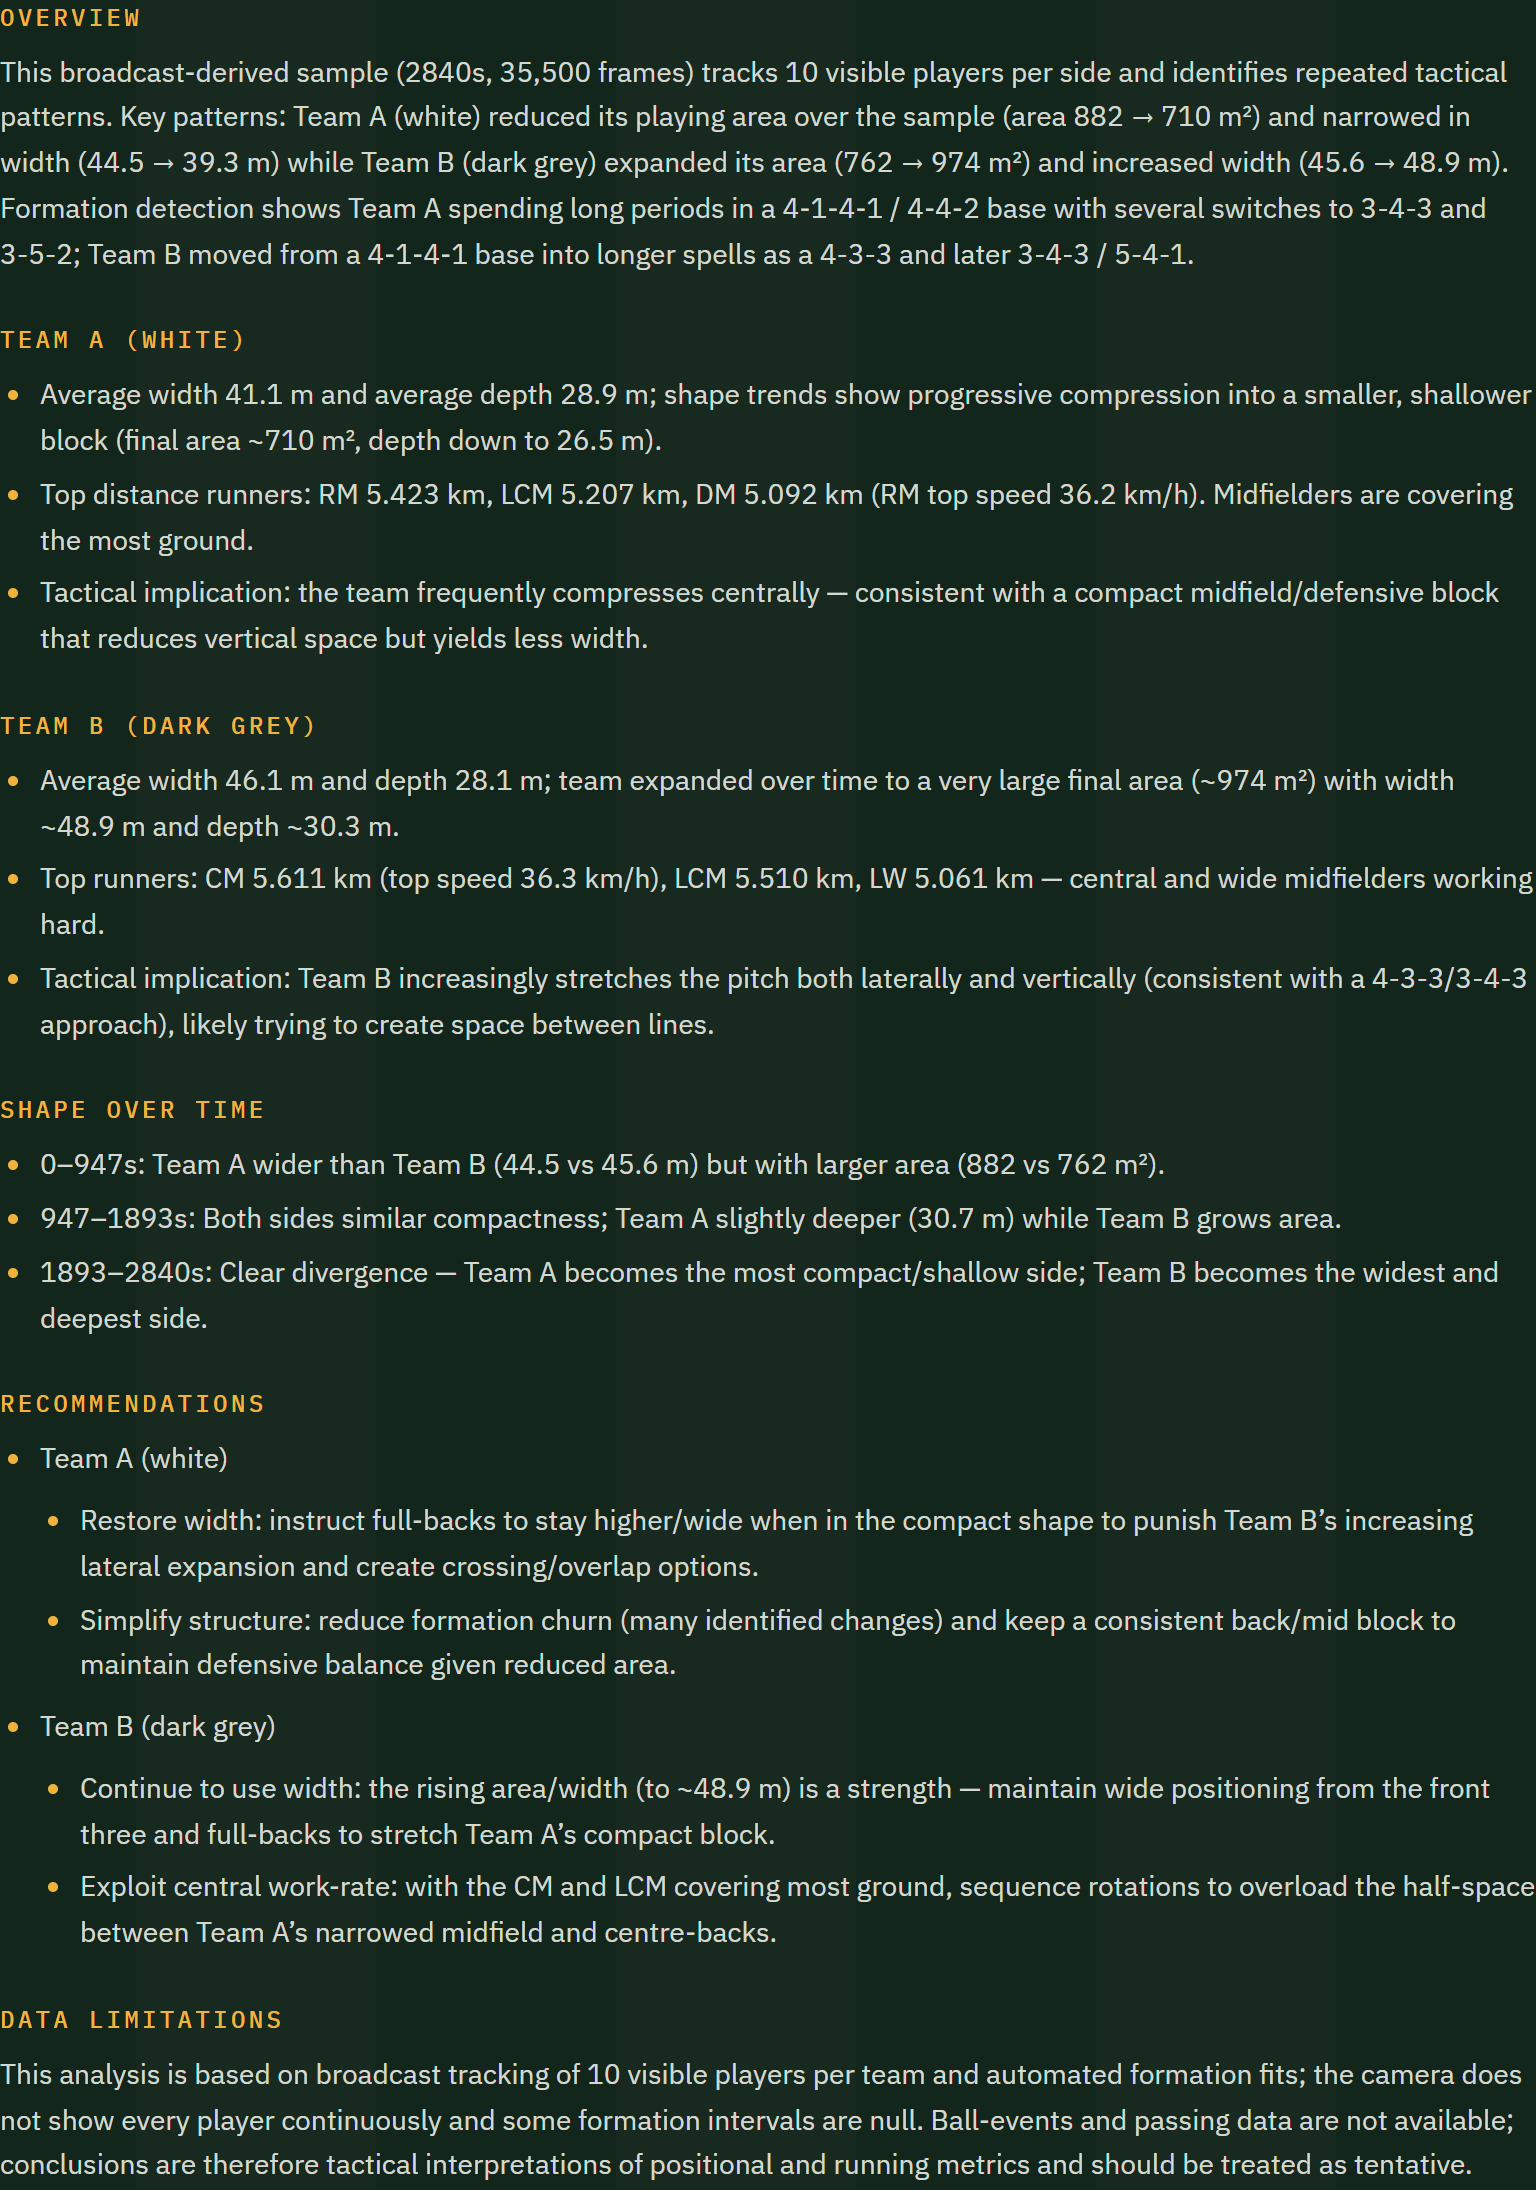
\includegraphics[width=0.82\textwidth]{21_coaching_report}
	\caption{The AI coaching report of the first half}
	\label{fig:report}
\end{figure}

\section{Re-analysing and deleting matches}
\label{sec:reanalyse-delete}

\emph{Re-analyse} (top right of the match page) queues the analysis of the stored video again, in the same mode. It is useful after a software update, after a failure or a cancellation. The previous results stay visible until the new analysis has finished.

\emph{Delete} in a match's row removes the match, its video and all results for good. It asks \emph{Delete?} with \emph{Yes} and \emph{No} first (\autoref{fig:delete}). A match that is being analysed cannot be deleted; it has to be cancelled first, or the user waits until it finishes. A match waiting in the queue can be deleted, and its job is removed from the queue.

\begin{figure}[H]
	\centering
	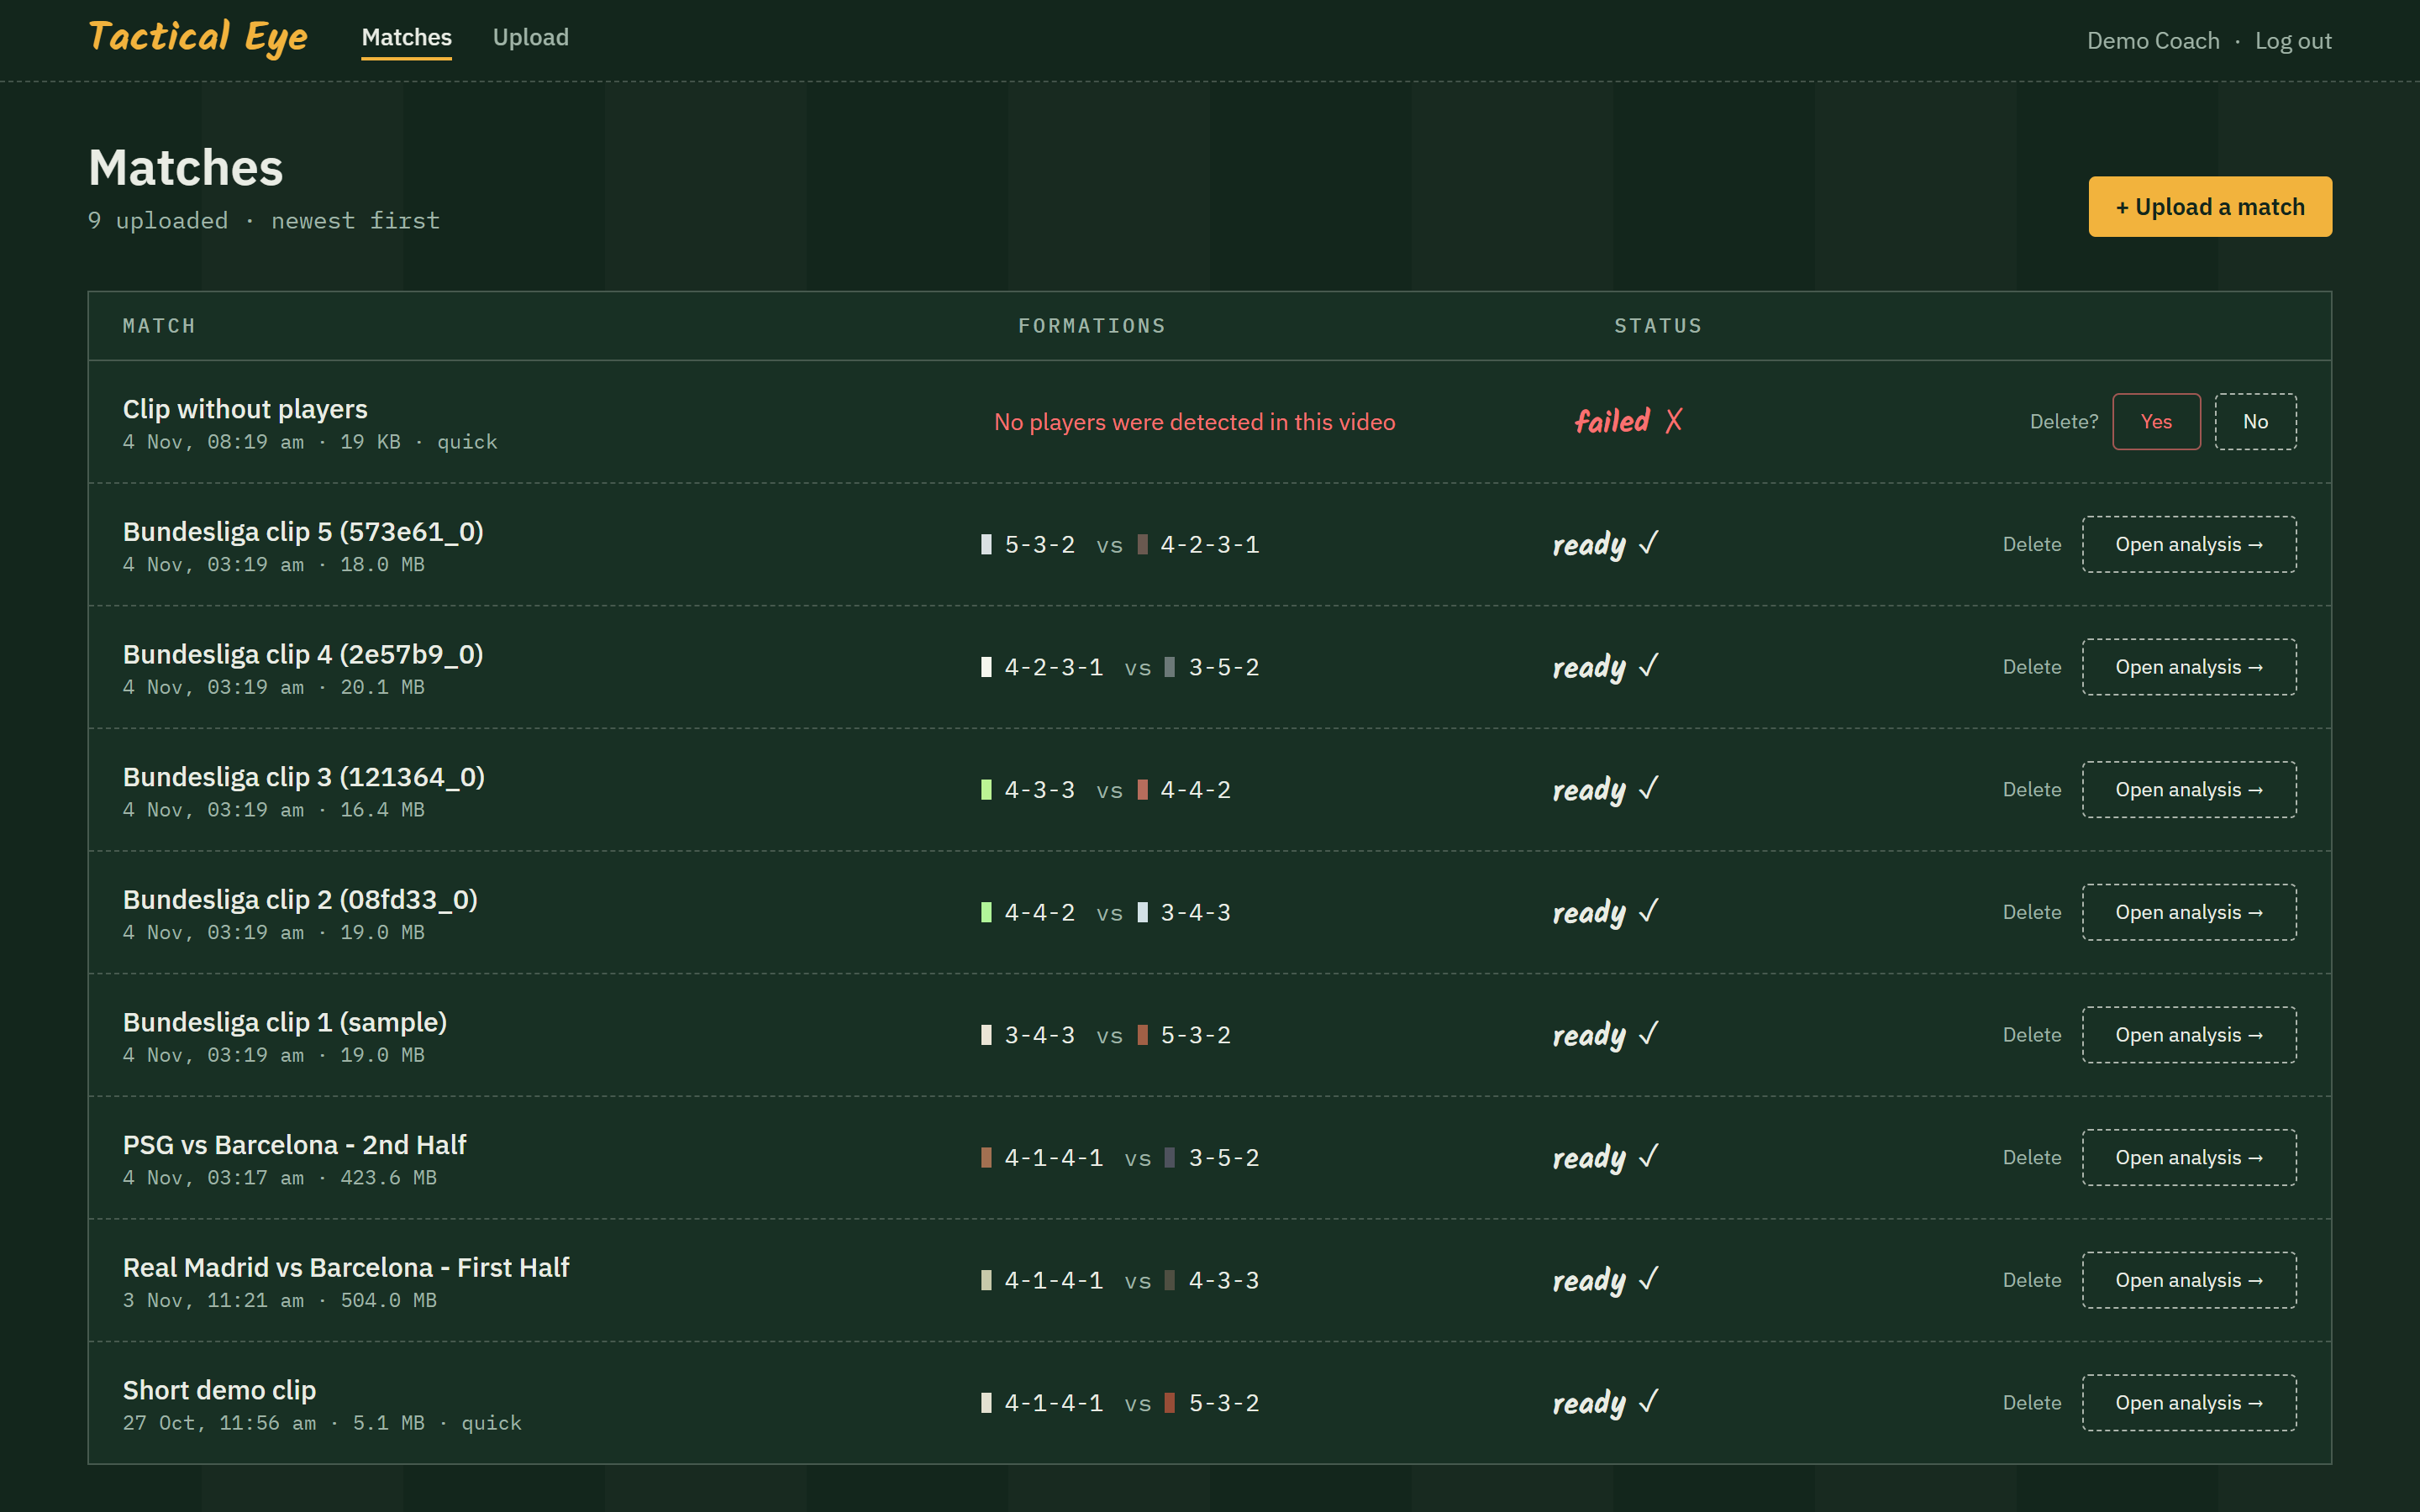
\includegraphics[width=\textwidth]{24_matches_failed_and_delete_confirm}
	\caption{A failed analysis and the delete confirmation}
	\label{fig:delete}
\end{figure}

\section{Messages and troubleshooting}
\label{sec:messages}

\subsection{Error messages}

Errors appear in red next to the action that caused them, or on the row and page of the affected match (\autoref{fig:failed}). \autoref{tab:errors} lists every error message and what to do about it.

\begin{figure}[H]
	\centering
	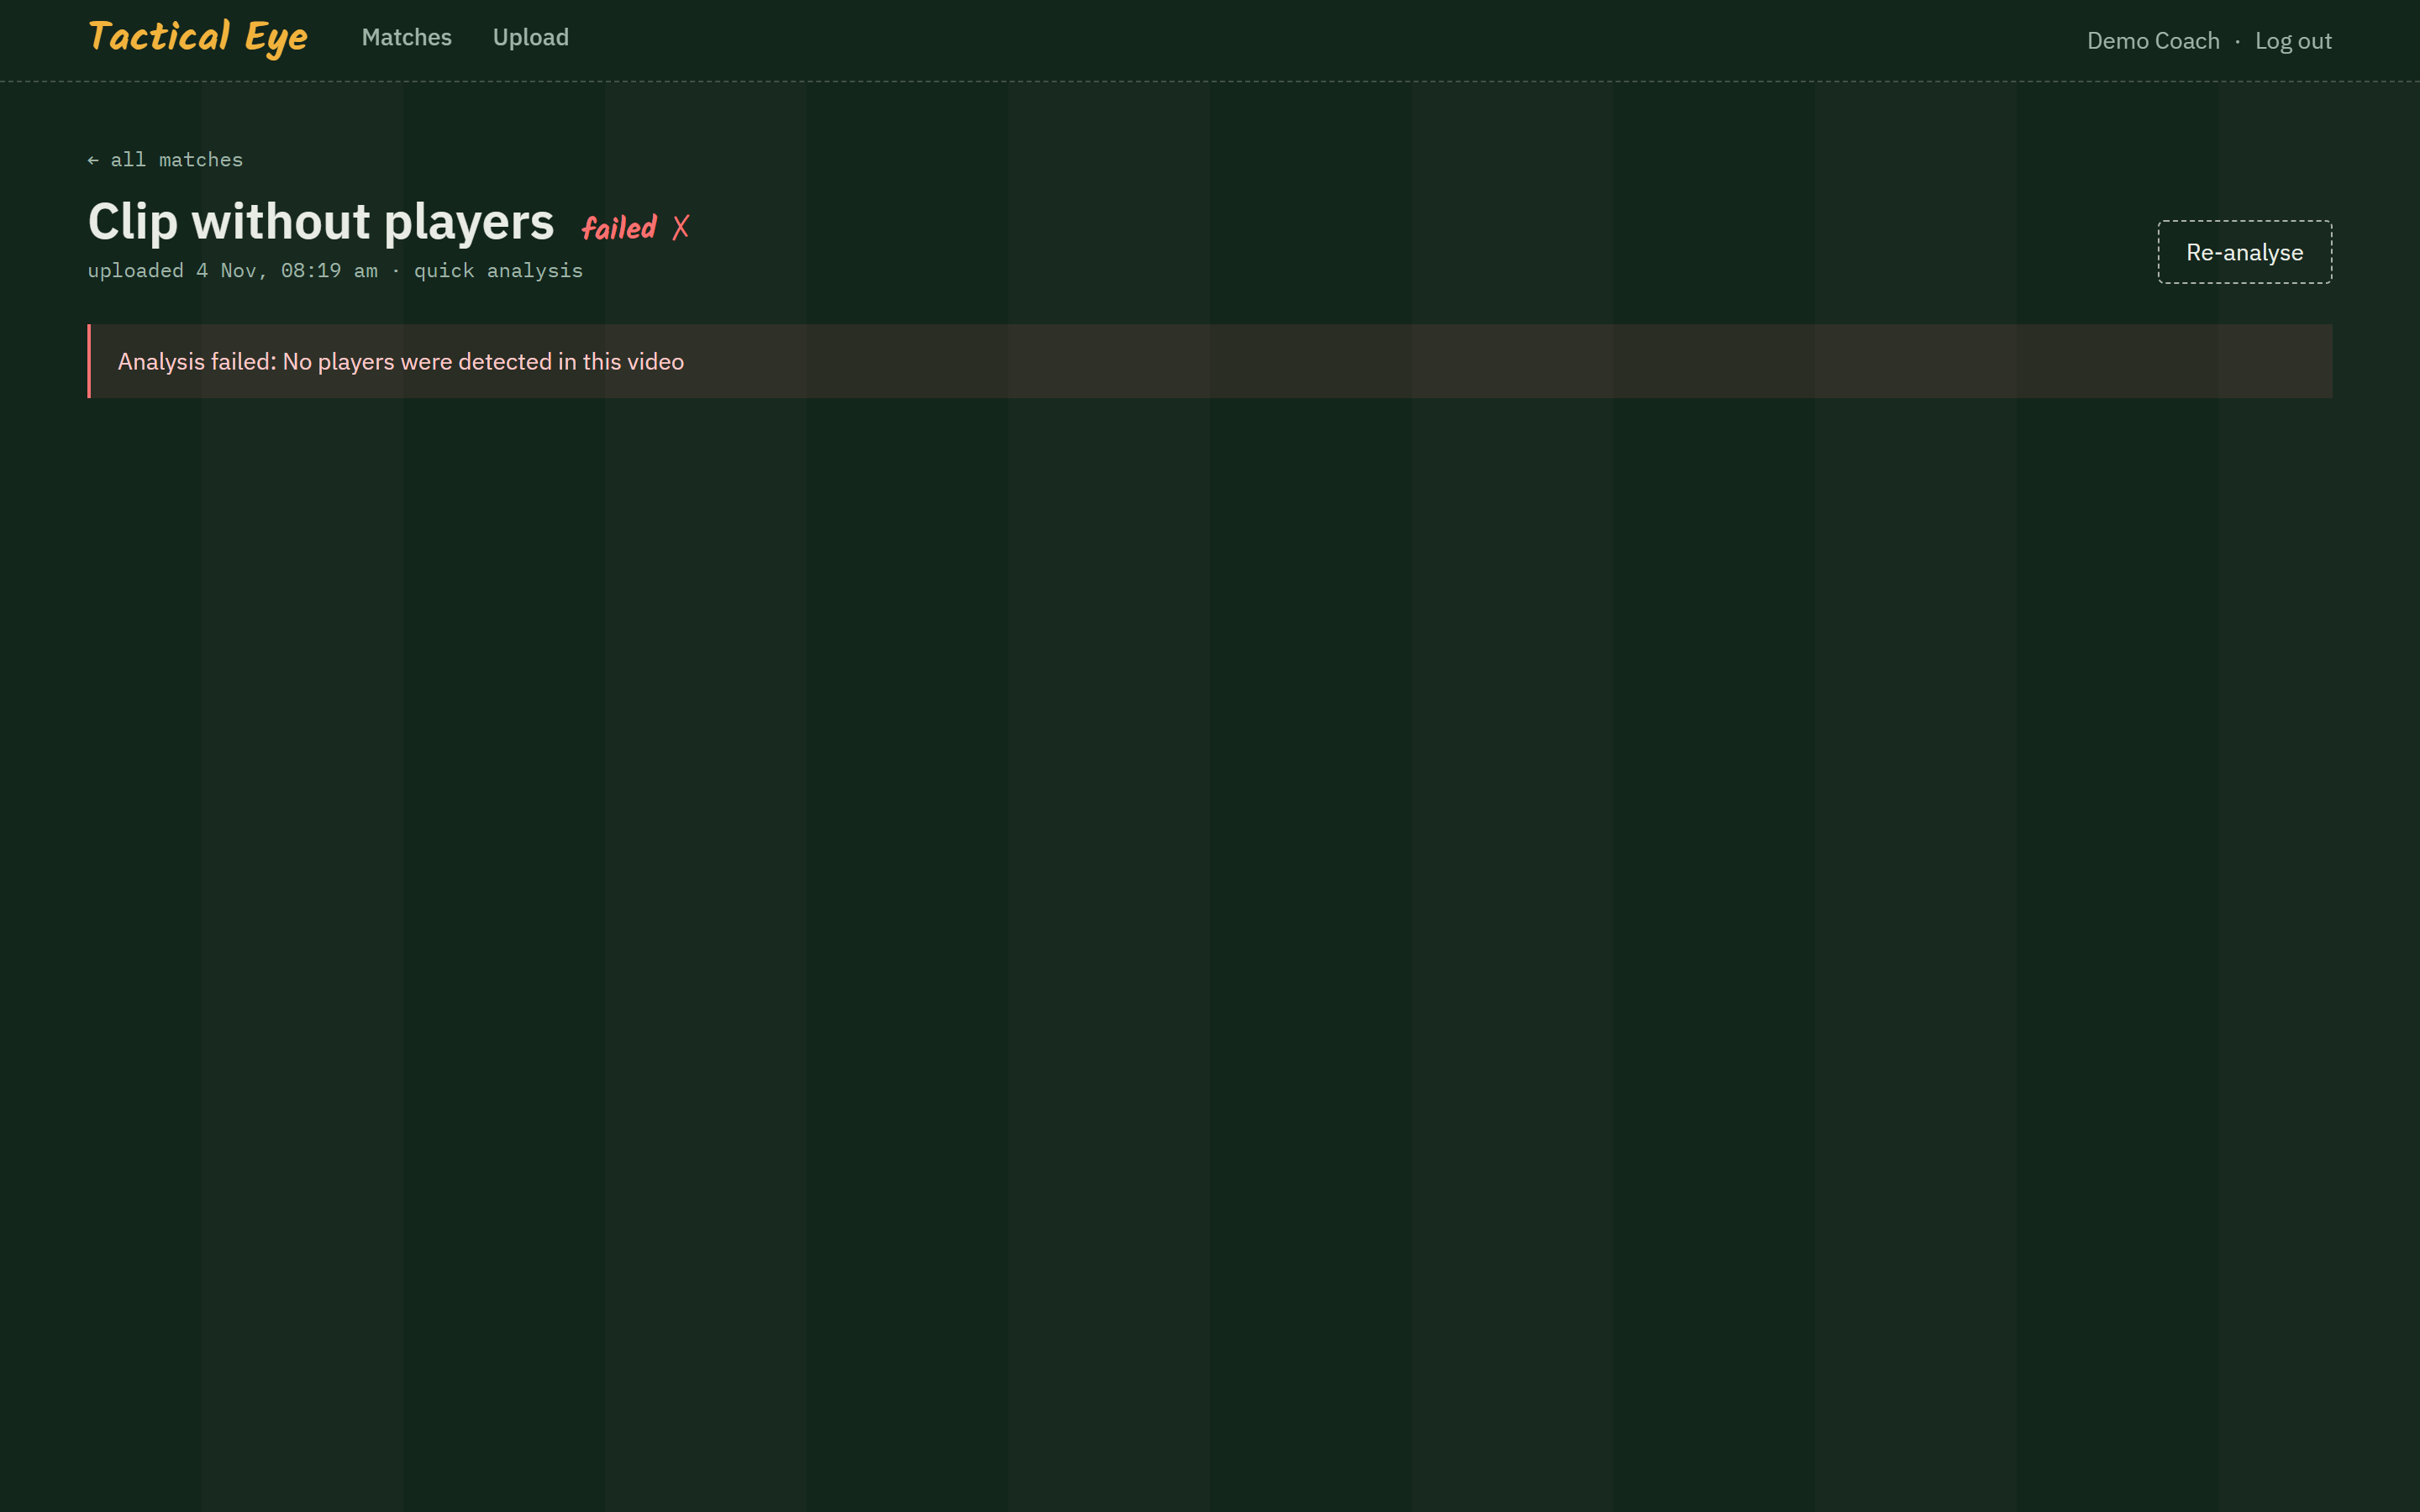
\includegraphics[width=\textwidth]{23_match_failed}
	\caption{The page of a match whose analysis failed}
	\label{fig:failed}
\end{figure}

\begin{longtable}{|p{0.33\textwidth}|p{0.29\textwidth}|p{0.29\textwidth}|}
	\hline
	\textbf{Message} & \textbf{Cause} & \textbf{What to do} \\
	\hline
	\endhead
	Invalid email or password & Wrong e-mail address or password at log-in. & Check both and try again. \\
	\hline
	An account with this email already exists & Registration with an address that is already used. & Log in instead, or use another address. \\
	\hline
	Password must be at least 8 characters & The registration password is too short. & Choose a longer password. \\
	\hline
	Upload a video file (.mp4, .mov, .m4v, .mkv, .webm, .avi) & No file was sent, or its extension or type is not a video. & Choose a file in one of the listed formats. \\
	\hline
	The file is not a valid video & The content is not a video, even though the name ends in a video extension. & Export or download the video again. \\
	\hline
	File is larger than 1024 MB & The upload exceeds the size limit. & Cut or compress the video, or ask the operator to raise \texttt{MAX\_\allowbreak{}UPLOAD\_\allowbreak{}MB}. \\
	\hline
	Network error during upload & The connection was lost during the upload. & Check the connection and upload again. \\
	\hline
	Could not queue the analysis job & The video was stored but the queue (Redis) was unreachable; the match is marked failed. & Operator: check the health address; then use Re-analyse. \\
	\hline
	No players were detected in this video & The analysis found no people, for example the video shows no football or only close-ups. & Use footage from the main broadcast camera. \\
	\hline
	Error, retrying: \dots{} / Retrying after an error & An attempt failed; it is retried once automatically. & Wait. If the second attempt fails too, the match becomes failed. \\
	\hline
	Match not found & The match was deleted, or the link belongs to another user's match. & Return to the match list. \\
	\hline
	This match is already being analysed & Re-analyse while the match is queued or being analysed. & Wait, or cancel the running analysis first. \\
	\hline
	This match is not being analysed & Cancel on a match that has already finished. & Nothing to do; reload the page. \\
	\hline
	This match is being analysed; cancel it first, or delete it when it finishes & Delete during the analysis. & Cancel the analysis, or wait until it finishes. \\
	\hline
	Analysis has not finished yet & Results or a report were requested before the analysis completed. & Wait until the match is ready. \\
	\hline
	The report service is busy; try again in a minute & The AI service limits how many requests it accepts. & Try again after a minute. \\
	\hline
	Could not reach the report service & No connection to Azure OpenAI. & Check the server's internet connection. \\
	\hline
	The Azure OpenAI key is invalid / Azure OpenAI deployment not found & The AI report is set up incorrectly. & Operator: correct the \texttt{AZURE\_\allowbreak{}OPENAI\_\allowbreak{}...} settings and restart the backend. \\
	\hline
	The report was blocked by the Azure content filter / The report came back empty / The report was cut off & The AI service did not return a usable report. & Click Regenerate. \\
	\hline
	Internal server error & An unexpected error on the server; the details go to the server log. & Try again; operator: read \texttt{docker compose logs backend}. \\
	\hline
	\caption{Error messages}
	\label{tab:errors}
\end{longtable}

\subsection{Information and warning messages}

\begin{table}[H]
	\centering
	\begin{tabular}{|p{0.50\textwidth}|p{0.42\textwidth}|}
		\hline
		\textbf{Message} & \textbf{Meaning} \\
		\hline
		No matches yet. & The user has not uploaded anything yet. \\
		\hline
		This page updates live. You can leave it; the analysis keeps running on the server. & Shown during the analysis. \\
		\hline
		Cancel this analysis? You can start it again later with Re-analyse. & Confirmation before cancelling. \\
		\hline
		The analysis was cancelled. Press Re-analyse to start it again. & The analysis was stopped by the user. \\
		\hline
		Click a player on the video or the board to see their movement, heatmap and physical stats. & No player is selected. \\
		\hline
		Paths and heatmaps on the video need a newer analysis of this match. & The match was analysed by an old version without per-frame camera geometry; Re-analyse fixes it. \\
		\hline
		Coaching reports are not configured on this server (Azure OpenAI settings are needed). & The operator has not enabled the AI report. \\
		\hline
		Analysing the statistics (about 10-30 seconds) & A report is being written. \\
		\hline
	\end{tabular}
	\caption{Information and warning messages}
	\label{tab:info-messages}
\end{table}

\subsection{Frequently asked questions}

\paragraph{The analysis is very slow.} On a CPU the analysis takes many times the length of the video. Quick mode helps for previews; for full halves, the cloud GPU service is the practical choice (\autoref{sec:cloud-gpu}).

\paragraph{The match stays queued.} No worker is running, or another match is being analysed first. The health address (\texttt{/api/health}) shows the number of workers; if it is 0, \texttt{docker compose --profile app up -d worker} starts the worker.

\paragraph{The labels change from one player to another.} Labels follow positions. When two players swap sides, their labels swap too, and a player who has only just come into view may have no label for a few seconds.

\paragraph{The formation looks wrong.} A formation needs at least 8 outfield players of the team to be visible in a 5-second window. When the runner-up is close, the team's shape really is between two formations.

\paragraph{The video does not play.} Every upload is converted into a format browsers can play. If the browser still cannot play it, an update of the browser usually helps; Chrome and Edge are recommended.

\subsection{Security and privacy}

Passwords are never stored, only a salted bcrypt hash of them, and the session cookie cannot be read by scripts on the page. Users can only see, change, cancel and delete their own matches; links to other users' matches answer \emph{Match not found}. Uploaded files are checked for real video content and stored under random names. The AI report service receives only the computed statistics, never the video or personal data. When the platform is reachable from the internet, the operator should serve it over HTTPS, for example behind a reverse proxy with a certificate, and keep \texttt{COOKIE\_\allowbreak{}SECURE} at its default.
